\documentclass[twoside]{book}

% Packages required by doxygen
\usepackage{fixltx2e}
\usepackage{calc}
\usepackage{doxygen}
\usepackage[export]{adjustbox} % also loads graphicx
\usepackage{graphicx}
\usepackage[utf8]{inputenc}
\usepackage{makeidx}
\usepackage{multicol}
\usepackage{multirow}
\PassOptionsToPackage{warn}{textcomp}
\usepackage{textcomp}
\usepackage[nointegrals]{wasysym}
\usepackage[table]{xcolor}

% Font selection
\usepackage[T1]{fontenc}
\usepackage[scaled=.90]{helvet}
\usepackage{courier}
\usepackage{amssymb}
\usepackage{sectsty}
\renewcommand{\familydefault}{\sfdefault}
\allsectionsfont{%
  \fontseries{bc}\selectfont%
  \color{darkgray}%
}
\renewcommand{\DoxyLabelFont}{%
  \fontseries{bc}\selectfont%
  \color{darkgray}%
}
\newcommand{\+}{\discretionary{\mbox{\scriptsize$\hookleftarrow$}}{}{}}

% Page & text layout
\usepackage{geometry}
\geometry{%
  a4paper,%
  top=2.5cm,%
  bottom=2.5cm,%
  left=2.5cm,%
  right=2.5cm%
}
\tolerance=750
\hfuzz=15pt
\hbadness=750
\setlength{\emergencystretch}{15pt}
\setlength{\parindent}{0cm}
\setlength{\parskip}{3ex plus 2ex minus 2ex}
\makeatletter
\renewcommand{\paragraph}{%
  \@startsection{paragraph}{4}{0ex}{-1.0ex}{1.0ex}{%
    \normalfont\normalsize\bfseries\SS@parafont%
  }%
}
\renewcommand{\subparagraph}{%
  \@startsection{subparagraph}{5}{0ex}{-1.0ex}{1.0ex}{%
    \normalfont\normalsize\bfseries\SS@subparafont%
  }%
}
\makeatother

% Headers & footers
\usepackage{fancyhdr}
\pagestyle{fancyplain}
\fancyhead[LE]{\fancyplain{}{\bfseries\thepage}}
\fancyhead[CE]{\fancyplain{}{}}
\fancyhead[RE]{\fancyplain{}{\bfseries\leftmark}}
\fancyhead[LO]{\fancyplain{}{\bfseries\rightmark}}
\fancyhead[CO]{\fancyplain{}{}}
\fancyhead[RO]{\fancyplain{}{\bfseries\thepage}}
\fancyfoot[LE]{\fancyplain{}{}}
\fancyfoot[CE]{\fancyplain{}{}}
\fancyfoot[RE]{\fancyplain{}{\bfseries\scriptsize Generated by Doxygen }}
\fancyfoot[LO]{\fancyplain{}{\bfseries\scriptsize Generated by Doxygen }}
\fancyfoot[CO]{\fancyplain{}{}}
\fancyfoot[RO]{\fancyplain{}{}}
\renewcommand{\footrulewidth}{0.4pt}
\renewcommand{\chaptermark}[1]{%
  \markboth{#1}{}%
}
\renewcommand{\sectionmark}[1]{%
  \markright{\thesection\ #1}%
}

% Indices & bibliography
\usepackage{natbib}
\usepackage[titles]{tocloft}
\setcounter{tocdepth}{3}
\setcounter{secnumdepth}{5}
\makeindex

% Hyperlinks (required, but should be loaded last)
\usepackage{ifpdf}
\ifpdf
  \usepackage[pdftex,pagebackref=true]{hyperref}
\else
  \usepackage[ps2pdf,pagebackref=true]{hyperref}
\fi
\hypersetup{%
  colorlinks=true,%
  linkcolor=blue,%
  citecolor=blue,%
  unicode%
}

% Custom commands
\newcommand{\clearemptydoublepage}{%
  \newpage{\pagestyle{empty}\cleardoublepage}%
}

\usepackage{caption}
\captionsetup{labelsep=space,justification=centering,font={bf},singlelinecheck=off,skip=4pt,position=top}

%===== C O N T E N T S =====

\begin{document}

% Titlepage & ToC
\hypersetup{pageanchor=false,
             bookmarksnumbered=true,
             pdfencoding=unicode
            }
\pagenumbering{roman}
\begin{titlepage}
\vspace*{7cm}
\begin{center}%
{\Large tracker \\[1ex]\large 0.\+0.\+0 }\\
\vspace*{1cm}
{\large Generated by Doxygen 1.8.11}\\
\end{center}
\end{titlepage}
\clearemptydoublepage
\tableofcontents
\clearemptydoublepage
\pagenumbering{arabic}
\hypersetup{pageanchor=true}

%--- Begin generated contents ---
\chapter{Tracker}
\label{md__home_travis_build_ManuelMeraz_Tracker_README}
\hypertarget{md__home_travis_build_ManuelMeraz_Tracker_README}{}
\href{https://travis-ci.com/ManuelMeraz/Tracker}{\tt }

\href{https://www.codefactor.io/repository/github/manuelmeraz/tracker/overview/master}{\tt }

Track my macronutrients, weight, and compute appropriate T\+D\+EE 
\chapter{Namespace Index}
\section{Namespace List}
Here is a list of all namespaces with brief descriptions\+:\begin{DoxyCompactList}
\item\contentsline{section}{\hyperlink{namespacedatabase}{database} \\*Organizes all databasing related classes and functions }{\pageref{namespacedatabase}}{}
\item\contentsline{section}{\hyperlink{namespacedatabase_1_1utils}{database\+::utils} \\*Utility functions to insert, retrieve, and manipulate objects in database }{\pageref{namespacedatabase_1_1utils}}{}
\item\contentsline{section}{\hyperlink{namespacefood}{food} \\*Organizes all food related classes and utilities }{\pageref{namespacefood}}{}
\end{DoxyCompactList}

\chapter{Hierarchical Index}
\section{Class Hierarchy}
This inheritance list is sorted roughly, but not completely, alphabetically\+:\begin{DoxyCompactList}
\item allocator\begin{DoxyCompactList}
\item \contentsline{section}{food\+:\+:Food\+:\+:Allocator}{\pageref{structfood_1_1_food_1_1_allocator}}{}
\end{DoxyCompactList}
\item \contentsline{section}{food\+:\+:Carbohydrate}{\pageref{structfood_1_1_carbohydrate}}{}
\item \contentsline{section}{database\+:\+:Column\+Properties}{\pageref{structdatabase_1_1_column_properties}}{}
\item \contentsline{section}{database\+:\+:Data}{\pageref{structdatabase_1_1_data}}{}
\item \contentsline{section}{database\+:\+:Database}{\pageref{classdatabase_1_1_database}}{}
\item \contentsline{section}{food\+:\+:Fat}{\pageref{structfood_1_1_fat}}{}
\item \contentsline{section}{food\+:\+:Fiber}{\pageref{structfood_1_1_fiber}}{}
\item \contentsline{section}{food\+:\+:Macronutrients}{\pageref{classfood_1_1_macronutrients}}{}
\item \contentsline{section}{food\+:\+:Protein}{\pageref{structfood_1_1_protein}}{}
\item \contentsline{section}{food\+:\+:Food\+:\+:Allocator\+:\+:rebind$<$ Food $>$}{\pageref{structfood_1_1_food_1_1_allocator_1_1rebind}}{}
\item \contentsline{section}{database\+:\+:Row}{\pageref{structdatabase_1_1_row}}{}
\item \contentsline{section}{database\+:\+:Storable}{\pageref{classdatabase_1_1_storable}}{}
\begin{DoxyCompactList}
\item \contentsline{section}{food\+:\+:Food}{\pageref{classfood_1_1_food}}{}
\end{DoxyCompactList}
\item Conan\+File\begin{DoxyCompactList}
\item \contentsline{section}{conanfile.\+Soci\+Test\+Conan}{\pageref{classconanfile_1_1_soci_test_conan}}{}
\end{DoxyCompactList}
\end{DoxyCompactList}

\chapter{Class Index}
\section{Class List}
Here are the classes, structs, unions and interfaces with brief descriptions\+:\begin{DoxyCompactList}
\item\contentsline{section}{\hyperlink{structfood_1_1_food_1_1_allocator}{food\+::\+Food\+::\+Allocator} \\*Custom allocator that allows database utils to own a vector of storable objects with private constructors }{\pageref{structfood_1_1_food_1_1_allocator}}{}
\item\contentsline{section}{\hyperlink{structfood_1_1_carbohydrate}{food\+::\+Carbohydrate} \\*Stores the carbohydrate content of a food }{\pageref{structfood_1_1_carbohydrate}}{}
\item\contentsline{section}{\hyperlink{structdatabase_1_1_column_properties}{database\+::\+Column\+Properties} \\*The column properties for a column in a table. A group of these represents a schema }{\pageref{structdatabase_1_1_column_properties}}{}
\item\contentsline{section}{\hyperlink{structdatabase_1_1_data}{database\+::\+Data} \\*The data to be stored into a database }{\pageref{structdatabase_1_1_data}}{}
\item\contentsline{section}{\hyperlink{classdatabase_1_1_database}{database\+::\+Database} \\*The database singleton class is in charge all database queries }{\pageref{classdatabase_1_1_database}}{}
\item\contentsline{section}{\hyperlink{structfood_1_1_fat}{food\+::\+Fat} \\*Stores the fat content of a food }{\pageref{structfood_1_1_fat}}{}
\item\contentsline{section}{\hyperlink{structfood_1_1_fiber}{food\+::\+Fiber} \\*Stores the fiber content of a food }{\pageref{structfood_1_1_fiber}}{}
\item\contentsline{section}{\hyperlink{classfood_1_1_food}{food\+::\+Food} \\*The food class stores all macronutrient and micronutrient data for any food }{\pageref{classfood_1_1_food}}{}
\item\contentsline{section}{\hyperlink{classfood_1_1_macronutrients}{food\+::\+Macronutrients} \\*The macronutrients class stores all macronutrient data to be stored in a \hyperlink{classfood_1_1_food}{Food} object }{\pageref{classfood_1_1_macronutrients}}{}
\item\contentsline{section}{\hyperlink{structfood_1_1_protein}{food\+::\+Protein} \\*Stores the protein content of a food }{\pageref{structfood_1_1_protein}}{}
\item\contentsline{section}{\hyperlink{structfood_1_1_food_1_1_allocator_1_1rebind}{food\+::\+Food\+::\+Allocator\+::rebind$<$ Food $>$} }{\pageref{structfood_1_1_food_1_1_allocator_1_1rebind}}{}
\item\contentsline{section}{\hyperlink{structdatabase_1_1_row}{database\+::\+Row} \\*A row of variant data }{\pageref{structdatabase_1_1_row}}{}
\item\contentsline{section}{\hyperlink{classdatabase_1_1_storable}{database\+::\+Storable} }{\pageref{classdatabase_1_1_storable}}{}
\end{DoxyCompactList}

\chapter{File Index}
\section{File List}
Here is a list of all files with brief descriptions\+:\begin{DoxyCompactList}
\item\contentsline{section}{/home/travis/build/\+Manuel\+Meraz/\+Tracker/\hyperlink{conanfile_8py}{conanfile.\+py} }{\pageref{conanfile_8py}}{}
\item\contentsline{section}{/home/travis/build/\+Manuel\+Meraz/\+Tracker/build/\hyperlink{_dart_configuration_8tcl}{Dart\+Configuration.\+tcl} }{\pageref{_dart_configuration_8tcl}}{}
\item\contentsline{section}{/home/travis/build/\+Manuel\+Meraz/\+Tracker/build/\+C\+Make\+Files/\hyperlink{feature__tests_8cxx}{feature\+\_\+tests.\+cxx} }{\pageref{feature__tests_8cxx}}{}
\item\contentsline{section}{/home/travis/build/\+Manuel\+Meraz/\+Tracker/build/\+C\+Make\+Files/3.\+12.\+4/\+Compiler\+Id\+C\+X\+X/\hyperlink{_c_make_c_x_x_compiler_id_8cpp}{C\+Make\+C\+X\+X\+Compiler\+Id.\+cpp} }{\pageref{_c_make_c_x_x_compiler_id_8cpp}}{}
\item\contentsline{section}{/home/travis/build/\+Manuel\+Meraz/\+Tracker/build/\+C\+Make\+Files/\+Check\+Library\+Exists/\hyperlink{_check_function_exists_8cxx}{Check\+Function\+Exists.\+cxx} }{\pageref{_check_function_exists_8cxx}}{}
\item\contentsline{section}{/home/travis/build/\+Manuel\+Meraz/\+Tracker/build/src/food/cotire/\hyperlink{food___c_x_x__prefix_8cxx}{food\+\_\+\+C\+X\+X\+\_\+prefix.\+cxx} }{\pageref{food___c_x_x__prefix_8cxx}}{}
\item\contentsline{section}{/home/travis/build/\+Manuel\+Meraz/\+Tracker/build/src/food/cotire/\hyperlink{food___c_x_x__prefix_8hxx}{food\+\_\+\+C\+X\+X\+\_\+prefix.\+hxx} }{\pageref{food___c_x_x__prefix_8hxx}}{}
\item\contentsline{section}{/home/travis/build/\+Manuel\+Meraz/\+Tracker/build/src/food/cotire/\hyperlink{food___c_x_x__unity_8cxx}{food\+\_\+\+C\+X\+X\+\_\+unity.\+cxx} }{\pageref{food___c_x_x__unity_8cxx}}{}
\item\contentsline{section}{/home/travis/build/\+Manuel\+Meraz/\+Tracker/include/database/\hyperlink{_data_8hpp}{Data.\+hpp} \\*The container for all data to be stored into a database }{\pageref{_data_8hpp}}{}
\item\contentsline{section}{/home/travis/build/\+Manuel\+Meraz/\+Tracker/include/database/\hyperlink{_database_8hpp}{Database.\+hpp} \\*Due to the way S\+Q\+Lite works, we want a single connection to the database up and running at all times. This class keeps the connection maintained }{\pageref{_database_8hpp}}{}
\item\contentsline{section}{/home/travis/build/\+Manuel\+Meraz/\+Tracker/include/database/\hyperlink{_storable_8hpp}{Storable.\+hpp} \\*The base class that all storable data will inherit from }{\pageref{_storable_8hpp}}{}
\item\contentsline{section}{/home/travis/build/\+Manuel\+Meraz/\+Tracker/include/database/\hyperlink{utils_8hpp}{utils.\+hpp} \\*Utility functions and objects for databasing }{\pageref{utils_8hpp}}{}
\item\contentsline{section}{/home/travis/build/\+Manuel\+Meraz/\+Tracker/include/food/\hyperlink{_food_8hpp}{Food.\+hpp} \\*The food class stores all macronutrient and micronutrient data for any food }{\pageref{_food_8hpp}}{}
\item\contentsline{section}{/home/travis/build/\+Manuel\+Meraz/\+Tracker/include/food/\hyperlink{_macronutrients_8hpp}{Macronutrients.\+hpp} }{\pageref{_macronutrients_8hpp}}{}
\item\contentsline{section}{/home/travis/build/\+Manuel\+Meraz/\+Tracker/src/\hyperlink{main_8cpp}{main.\+cpp} }{\pageref{main_8cpp}}{}
\item\contentsline{section}{/home/travis/build/\+Manuel\+Meraz/\+Tracker/src/database/\hyperlink{_database_8cpp}{Database.\+cpp} \\*The database singleton class is in charge all database queries }{\pageref{_database_8cpp}}{}
\item\contentsline{section}{/home/travis/build/\+Manuel\+Meraz/\+Tracker/src/food/\hyperlink{_food_8cpp}{Food.\+cpp} \\*The food class stores all macronutrient and micronutrient data for any food }{\pageref{_food_8cpp}}{}
\item\contentsline{section}{/home/travis/build/\+Manuel\+Meraz/\+Tracker/src/food/\hyperlink{_macronutrients_8cpp}{Macronutrients.\+cpp} \\*Contains the Macronutrients class and related helper classes food }{\pageref{_macronutrients_8cpp}}{}
\item\contentsline{section}{/home/travis/build/\+Manuel\+Meraz/\+Tracker/tests/\hyperlink{test-food_8cpp}{test-\/food.\+cpp} }{\pageref{test-food_8cpp}}{}
\item\contentsline{section}{/home/travis/build/\+Manuel\+Meraz/\+Tracker/tools/\hyperlink{build_8py}{build.\+py} }{\pageref{build_8py}}{}
\item\contentsline{section}{/home/travis/build/\+Manuel\+Meraz/\+Tracker/tools/\hyperlink{format__code_8py}{format\+\_\+code.\+py} }{\pageref{format__code_8py}}{}
\item\contentsline{section}{/home/travis/build/\+Manuel\+Meraz/\+Tracker/tools/clang-\/tools/\hyperlink{clang-tidy-diff_8py}{clang-\/tidy-\/diff.\+py} }{\pageref{clang-tidy-diff_8py}}{}
\item\contentsline{section}{/home/travis/build/\+Manuel\+Meraz/\+Tracker/tools/clang-\/tools/\hyperlink{run-clang-tidy_8py}{run-\/clang-\/tidy.\+py} }{\pageref{run-clang-tidy_8py}}{}
\end{DoxyCompactList}

\chapter{Namespace Documentation}
\hypertarget{namespacedatabase}{}\section{database Namespace Reference}
\label{namespacedatabase}\index{database@{database}}


Organizes all databasing related classes and functions.  


\subsection*{Namespaces}
\begin{DoxyCompactItemize}
\item 
 \hyperlink{namespacedatabase_1_1utils}{utils}
\begin{DoxyCompactList}\small\item\em Utility functions to insert, retrieve, and manipulate objects in database. \end{DoxyCompactList}\end{DoxyCompactItemize}
\subsection*{Classes}
\begin{DoxyCompactItemize}
\item 
struct \hyperlink{structdatabase_1_1_column_properties}{Column\+Properties}
\begin{DoxyCompactList}\small\item\em The column properties for a column in a table. A group of these represents a schema. \end{DoxyCompactList}\item 
struct \hyperlink{structdatabase_1_1_data}{Data}
\begin{DoxyCompactList}\small\item\em The data to be stored into a database. \end{DoxyCompactList}\item 
class \hyperlink{classdatabase_1_1_database}{Database}
\begin{DoxyCompactList}\small\item\em The database singleton class is in charge all database queries. \end{DoxyCompactList}\item 
struct \hyperlink{structdatabase_1_1_row}{Row}
\begin{DoxyCompactList}\small\item\em A row of variant data. \end{DoxyCompactList}\item 
class \hyperlink{classdatabase_1_1_storable}{Storable}
\end{DoxyCompactItemize}
\subsection*{Enumerations}
\begin{DoxyCompactItemize}
\item 
enum \hyperlink{namespacedatabase_a596cea80c57ec5a9b3b4018f733a43fd}{Data\+Type} \{ \\*
\hyperlink{namespacedatabase_a596cea80c57ec5a9b3b4018f733a43fda8cf125b0e31559ba75a9d9b4f818a554}{Data\+Type\+::\+R\+E\+AL}, 
\hyperlink{namespacedatabase_a596cea80c57ec5a9b3b4018f733a43fda5d5cd46919fa987731fb2edefe0f2a0c}{Data\+Type\+::\+I\+N\+T\+E\+G\+ER}, 
\hyperlink{namespacedatabase_a596cea80c57ec5a9b3b4018f733a43fda61a96ffcb251bb9bf0abf8fec19d0ea8}{Data\+Type\+::\+T\+E\+XT}, 
\hyperlink{namespacedatabase_a596cea80c57ec5a9b3b4018f733a43fda6d67bdfe4ae19f38aff8f363bca42892}{Data\+Type\+::\+N\+U\+L\+L\+\_\+}, 
\\*
\hyperlink{namespacedatabase_a596cea80c57ec5a9b3b4018f733a43fda1649cff06611a6025da3dd511a97fb43}{Data\+Type\+::\+B\+L\+OB}
 \}\begin{DoxyCompactList}\small\item\em S\+QL datatypes that could be stored into a database. \end{DoxyCompactList}
\item 
enum \hyperlink{namespacedatabase_a77defe1118948f64f1e32f4b78c04f5b}{Constraint} \{ \hyperlink{namespacedatabase_a77defe1118948f64f1e32f4b78c04f5ba5e0276ef8ae59ebb9aae19348ad173d5}{Constraint\+::\+P\+R\+I\+M\+A\+R\+Y\+\_\+\+K\+EY}, 
\hyperlink{namespacedatabase_a77defe1118948f64f1e32f4b78c04f5ba88e3e8040c7cd11b9faffdf34372fa2a}{Constraint\+::\+U\+N\+I\+Q\+UE}, 
\hyperlink{namespacedatabase_a77defe1118948f64f1e32f4b78c04f5baeed1de8e53bda49dda97e42841cfe6c5}{Constraint\+::\+N\+O\+T\+\_\+\+N\+U\+LL}, 
\hyperlink{namespacedatabase_a77defe1118948f64f1e32f4b78c04f5ba8c46d8d9d3402788403e2f6911153089}{Constraint\+::\+C\+H\+E\+CK}
 \}\begin{DoxyCompactList}\small\item\em The S\+QL constraint for column of data when creating a table schema. \end{DoxyCompactList}
\end{DoxyCompactItemize}


\subsection{Detailed Description}
Organizes all databasing related classes and functions. 

\subsection{Enumeration Type Documentation}
\index{database@{database}!Constraint@{Constraint}}
\index{Constraint@{Constraint}!database@{database}}
\subsubsection[{\texorpdfstring{Constraint}{Constraint}}]{\setlength{\rightskip}{0pt plus 5cm}enum {\bf database\+::\+Constraint}\hspace{0.3cm}{\ttfamily [strong]}}\hypertarget{namespacedatabase_a77defe1118948f64f1e32f4b78c04f5b}{}\label{namespacedatabase_a77defe1118948f64f1e32f4b78c04f5b}


The S\+QL constraint for column of data when creating a table schema. 

\begin{Desc}
\item[Enumerator]\par
\begin{description}
\index{P\+R\+I\+M\+A\+R\+Y\+\_\+\+K\+EY@{P\+R\+I\+M\+A\+R\+Y\+\_\+\+K\+EY}!database@{database}}\index{database@{database}!P\+R\+I\+M\+A\+R\+Y\+\_\+\+K\+EY@{P\+R\+I\+M\+A\+R\+Y\+\_\+\+K\+EY}}\item[{\em 
P\+R\+I\+M\+A\+R\+Y\+\_\+\+K\+EY\hypertarget{namespacedatabase_a77defe1118948f64f1e32f4b78c04f5ba5e0276ef8ae59ebb9aae19348ad173d5}{}\label{namespacedatabase_a77defe1118948f64f1e32f4b78c04f5ba5e0276ef8ae59ebb9aae19348ad173d5}
}]\index{U\+N\+I\+Q\+UE@{U\+N\+I\+Q\+UE}!database@{database}}\index{database@{database}!U\+N\+I\+Q\+UE@{U\+N\+I\+Q\+UE}}\item[{\em 
U\+N\+I\+Q\+UE\hypertarget{namespacedatabase_a77defe1118948f64f1e32f4b78c04f5ba88e3e8040c7cd11b9faffdf34372fa2a}{}\label{namespacedatabase_a77defe1118948f64f1e32f4b78c04f5ba88e3e8040c7cd11b9faffdf34372fa2a}
}]\index{N\+O\+T\+\_\+\+N\+U\+LL@{N\+O\+T\+\_\+\+N\+U\+LL}!database@{database}}\index{database@{database}!N\+O\+T\+\_\+\+N\+U\+LL@{N\+O\+T\+\_\+\+N\+U\+LL}}\item[{\em 
N\+O\+T\+\_\+\+N\+U\+LL\hypertarget{namespacedatabase_a77defe1118948f64f1e32f4b78c04f5baeed1de8e53bda49dda97e42841cfe6c5}{}\label{namespacedatabase_a77defe1118948f64f1e32f4b78c04f5baeed1de8e53bda49dda97e42841cfe6c5}
}]\index{C\+H\+E\+CK@{C\+H\+E\+CK}!database@{database}}\index{database@{database}!C\+H\+E\+CK@{C\+H\+E\+CK}}\item[{\em 
C\+H\+E\+CK\hypertarget{namespacedatabase_a77defe1118948f64f1e32f4b78c04f5ba8c46d8d9d3402788403e2f6911153089}{}\label{namespacedatabase_a77defe1118948f64f1e32f4b78c04f5ba8c46d8d9d3402788403e2f6911153089}
}]\end{description}
\end{Desc}
\index{database@{database}!Data\+Type@{Data\+Type}}
\index{Data\+Type@{Data\+Type}!database@{database}}
\subsubsection[{\texorpdfstring{Data\+Type}{DataType}}]{\setlength{\rightskip}{0pt plus 5cm}enum {\bf database\+::\+Data\+Type}\hspace{0.3cm}{\ttfamily [strong]}}\hypertarget{namespacedatabase_a596cea80c57ec5a9b3b4018f733a43fd}{}\label{namespacedatabase_a596cea80c57ec5a9b3b4018f733a43fd}


S\+QL datatypes that could be stored into a database. 

Types with the underscore \+\_\+ suffix were special keywords that could not be defined. \begin{Desc}
\item[Enumerator]\par
\begin{description}
\index{R\+E\+AL@{R\+E\+AL}!database@{database}}\index{database@{database}!R\+E\+AL@{R\+E\+AL}}\item[{\em 
R\+E\+AL\hypertarget{namespacedatabase_a596cea80c57ec5a9b3b4018f733a43fda8cf125b0e31559ba75a9d9b4f818a554}{}\label{namespacedatabase_a596cea80c57ec5a9b3b4018f733a43fda8cf125b0e31559ba75a9d9b4f818a554}
}]\index{I\+N\+T\+E\+G\+ER@{I\+N\+T\+E\+G\+ER}!database@{database}}\index{database@{database}!I\+N\+T\+E\+G\+ER@{I\+N\+T\+E\+G\+ER}}\item[{\em 
I\+N\+T\+E\+G\+ER\hypertarget{namespacedatabase_a596cea80c57ec5a9b3b4018f733a43fda5d5cd46919fa987731fb2edefe0f2a0c}{}\label{namespacedatabase_a596cea80c57ec5a9b3b4018f733a43fda5d5cd46919fa987731fb2edefe0f2a0c}
}]\index{T\+E\+XT@{T\+E\+XT}!database@{database}}\index{database@{database}!T\+E\+XT@{T\+E\+XT}}\item[{\em 
T\+E\+XT\hypertarget{namespacedatabase_a596cea80c57ec5a9b3b4018f733a43fda61a96ffcb251bb9bf0abf8fec19d0ea8}{}\label{namespacedatabase_a596cea80c57ec5a9b3b4018f733a43fda61a96ffcb251bb9bf0abf8fec19d0ea8}
}]\index{N\+U\+L\+L\+\_\+@{N\+U\+L\+L\+\_\+}!database@{database}}\index{database@{database}!N\+U\+L\+L\+\_\+@{N\+U\+L\+L\+\_\+}}\item[{\em 
N\+U\+L\+L\+\_\+\hypertarget{namespacedatabase_a596cea80c57ec5a9b3b4018f733a43fda6d67bdfe4ae19f38aff8f363bca42892}{}\label{namespacedatabase_a596cea80c57ec5a9b3b4018f733a43fda6d67bdfe4ae19f38aff8f363bca42892}
}]\index{B\+L\+OB@{B\+L\+OB}!database@{database}}\index{database@{database}!B\+L\+OB@{B\+L\+OB}}\item[{\em 
B\+L\+OB\hypertarget{namespacedatabase_a596cea80c57ec5a9b3b4018f733a43fda1649cff06611a6025da3dd511a97fb43}{}\label{namespacedatabase_a596cea80c57ec5a9b3b4018f733a43fda1649cff06611a6025da3dd511a97fb43}
}]\end{description}
\end{Desc}

\hypertarget{namespacedatabase_1_1utils}{}\section{database\+:\+:utils Namespace Reference}
\label{namespacedatabase_1_1utils}\index{database\+::utils@{database\+::utils}}


Utility functions to insert, retrieve, and manipulate objects in database.  


\subsection*{Functions}
\begin{DoxyCompactItemize}
\item 
{\footnotesize template$<$class Forward\+It , class T , class Compare  = std\+::less$<$$>$$>$ }\\auto \hyperlink{namespacedatabase_1_1utils_a0dd569af49c9913a5090b71c86690fe5}{binary\+\_\+find} (Forward\+It first, Forward\+It last, const T \&value, Compare comp) -\/$>$ Forward\+It
\begin{DoxyCompactList}\small\item\em Finds and returns the object if it exists in the stl container. \end{DoxyCompactList}\item 
{\footnotesize template$<$typename Storable , typename std\+::enable\+\_\+if\+\_\+t$<$ std\+::is\+\_\+base\+\_\+of\+\_\+v$<$ database\+::\+Storable, std\+::decay\+\_\+t$<$ Storable $>$$>$, int $>$  = 0$>$ }\\auto \hyperlink{namespacedatabase_1_1utils_adae24cb18f62390528243ff3218d8626}{count\+\_\+rows} () -\/$>$ size\+\_\+t
\begin{DoxyCompactList}\small\item\em Count the number of \hyperlink{classdatabase_1_1_storable}{Storable} type in the database. \end{DoxyCompactList}\item 
{\footnotesize template$<$typename Storable , typename std\+::enable\+\_\+if\+\_\+t$<$ std\+::is\+\_\+base\+\_\+of\+\_\+v$<$ database\+::\+Storable, std\+::decay\+\_\+t$<$ Storable $>$$>$, int $>$  = 0$>$ }\\void \hyperlink{namespacedatabase_1_1utils_a303b59245b11befd59f3fd0e838ef80b}{create\+\_\+table} (std\+::vector$<$ \hyperlink{structdatabase_1_1_column_properties}{Column\+Properties} $>$ const \&schema)
\begin{DoxyCompactList}\small\item\em Create table of \hyperlink{classdatabase_1_1_storable}{Storable} if not exists. \end{DoxyCompactList}\item 
{\footnotesize template$<$typename Storable , typename std\+::enable\+\_\+if\+\_\+t$<$ std\+::is\+\_\+base\+\_\+of\+\_\+v$<$ database\+::\+Storable, std\+::decay\+\_\+t$<$ Storable $>$$>$, int $>$  = 0$>$ }\\void \hyperlink{namespacedatabase_1_1utils_ac56bf4b6fc7b1481c84e42e6bb6db57b}{delete\+\_\+storable} (\hyperlink{classdatabase_1_1_storable}{Storable} const \&storable)
\begin{DoxyCompactList}\small\item\em Delete \hyperlink{classdatabase_1_1_storable}{Storable} object from datbase and cache of storables. \end{DoxyCompactList}\item 
{\footnotesize template$<$typename Storable , typename std\+::enable\+\_\+if\+\_\+t$<$ std\+::is\+\_\+base\+\_\+of\+\_\+v$<$ database\+::\+Storable, std\+::decay\+\_\+t$<$ Storable $>$$>$, int $>$  = 0$>$ }\\void \hyperlink{namespacedatabase_1_1utils_abfc70aa38436efb787b6c9f62941856d}{drop\+\_\+table} ()
\begin{DoxyCompactList}\small\item\em Deletes the \hyperlink{classdatabase_1_1_storable}{Storable} table from the database. \end{DoxyCompactList}\item 
{\footnotesize template$<$typename Data\+Enum , typename std\+::enable\+\_\+if\+\_\+t$<$ std\+::is\+\_\+enum\+\_\+v$<$ Data\+Enum $>$, int $>$  = 0$>$ }\\auto \hyperlink{namespacedatabase_1_1utils_a84e6b2503f6453631d2238ff3f9bc9e3}{enum\+\_\+to\+\_\+string} (Data\+Enum const \&data\+\_\+enum) -\/$>$ std\+::string\+\_\+view
\begin{DoxyCompactList}\small\item\em to\+\_\+string function for data enum types \end{DoxyCompactList}\item 
{\footnotesize template$<$typename Storable , typename std\+::enable\+\_\+if\+\_\+t$<$ std\+::is\+\_\+base\+\_\+of\+\_\+v$<$ database\+::\+Storable, std\+::decay\+\_\+t$<$ Storable $>$$>$, int $>$  = 0$>$ }\\auto \hyperlink{namespacedatabase_1_1utils_acab03452308a27ee3e8e5f30842d8ca8}{get\+\_\+new\+\_\+id} () -\/$>$ int
\begin{DoxyCompactList}\small\item\em Generates new unique ID for the type being asked for. \end{DoxyCompactList}\item 
{\footnotesize template$<$typename Storable , typename std\+::enable\+\_\+if\+\_\+t$<$ std\+::is\+\_\+base\+\_\+of\+\_\+v$<$ database\+::\+Storable, std\+::decay\+\_\+t$<$ Storable $>$$>$, int $>$  = 0$>$ }\\void \hyperlink{namespacedatabase_1_1utils_ab9b80f05cca7a094baf577ec5b62108c}{insert} (\hyperlink{classdatabase_1_1_storable}{Storable} const \&storable)
\begin{DoxyCompactList}\small\item\em Gets data from any storable object and inserts it into relevant database. \end{DoxyCompactList}\item 
{\footnotesize template$<$typename Storable , typename... Args, typename std\+::enable\+\_\+if\+\_\+t$<$ std\+::is\+\_\+base\+\_\+of\+\_\+v$<$ database\+::\+Storable, std\+::decay\+\_\+t$<$ Storable $>$$>$, int $>$  = 0$>$ }\\auto \hyperlink{namespacedatabase_1_1utils_a8d10f5dbf82b7d8008d8d82865c5a19a}{make} (Args \&\&...args) -\/$>$ \hyperlink{classdatabase_1_1_storable}{Storable} \&
\begin{DoxyCompactList}\small\item\em Generates a new \hyperlink{classdatabase_1_1_storable}{Storable} object stores it in the cache, inserts it into the database, and returns a reference to tht new object. \end{DoxyCompactList}\item 
{\footnotesize template$<$typename Storable , typename std\+::enable\+\_\+if\+\_\+t$<$ std\+::is\+\_\+base\+\_\+of\+\_\+v$<$ database\+::\+Storable, std\+::decay\+\_\+t$<$ Storable $>$$>$, int $>$  = 0$>$ }\\auto \hyperlink{namespacedatabase_1_1utils_a41142b70272ad4b4ec442a28dc5c8ce3}{retrieve\+\_\+all} () -\/$>$ std\+::vector$<$ \hyperlink{classdatabase_1_1_storable}{Storable}, struct Storable\+::\+Allocator $>$ \&
\begin{DoxyCompactList}\small\item\em Retrieves all database objects that match the \hyperlink{classdatabase_1_1_storable}{Storable} that is passed in. \end{DoxyCompactList}\item 
{\footnotesize template$<$typename Storable , typename std\+::enable\+\_\+if\+\_\+t$<$ std\+::is\+\_\+base\+\_\+of\+\_\+v$<$ database\+::\+Storable, std\+::decay\+\_\+t$<$ Storable $>$$>$, int $>$  = 0$>$ }\\auto \hyperlink{namespacedatabase_1_1utils_a3c5ce09d7fc593c4395d40fe5c1a0630}{table\+\_\+exists} () -\/$>$ bool
\begin{DoxyCompactList}\small\item\em Check if \hyperlink{classdatabase_1_1_storable}{Storable} table exists in database. \end{DoxyCompactList}\item 
{\footnotesize template$<$typename T $>$ }\\auto \hyperlink{namespacedatabase_1_1utils_acb264e8826f50ae828a9c89c2906b049}{type\+\_\+to\+\_\+string} () -\/$>$ std\+::string
\begin{DoxyCompactList}\small\item\em Converts a type to a string and trims the namespaces off. (e.\+g. namespace\+::other\+\_\+namespace\+::\+Class\+Name -\/$>$ \char`\"{}\+Class\+Name\char`\"{}) \end{DoxyCompactList}\item 
{\footnotesize template$<$typename Storable , typename std\+::enable\+\_\+if\+\_\+t$<$ std\+::is\+\_\+base\+\_\+of\+\_\+v$<$ database\+::\+Storable, std\+::decay\+\_\+t$<$ Storable $>$$>$, int $>$  = 0$>$ }\\void \hyperlink{namespacedatabase_1_1utils_ad7fc4b4d352c7b947fc48ac8c1d666a6}{update} (\hyperlink{classdatabase_1_1_storable}{Storable} const \&storable)
\begin{DoxyCompactList}\small\item\em Updates the \hyperlink{classdatabase_1_1_storable}{Storable} objects data within the database. \end{DoxyCompactList}\item 
{\footnotesize template$<$typename Lambda $>$ }\\void \hyperlink{namespacedatabase_1_1utils_a974d01a6dbb387b033f627d846630b92}{visit\+\_\+row\+\_\+data} (Lambda const \&handler, \hyperlink{structdatabase_1_1_row_a29c16186778c974af723db03751f3aa3}{Row\+::row\+\_\+data\+\_\+t} const \&row\+\_\+data)
\begin{DoxyCompactList}\small\item\em Updates the \hyperlink{classdatabase_1_1_storable}{Storable} objects data within the database. \end{DoxyCompactList}\end{DoxyCompactItemize}


\subsection{Detailed Description}
Utility functions to insert, retrieve, and manipulate objects in database. 

\subsection{Function Documentation}
\index{database\+::utils@{database\+::utils}!binary\+\_\+find@{binary\+\_\+find}}
\index{binary\+\_\+find@{binary\+\_\+find}!database\+::utils@{database\+::utils}}
\subsubsection[{\texorpdfstring{binary\+\_\+find(\+Forward\+It first, Forward\+It last, const T \&value, Compare comp) -\/$>$ Forward\+It}{binary_find(ForwardIt first, ForwardIt last, const T &value, Compare comp) -> ForwardIt}}]{\setlength{\rightskip}{0pt plus 5cm}template$<$class Forward\+It , class T , class Compare  = std\+::less$<$$>$$>$ auto database\+::utils\+::binary\+\_\+find (
\begin{DoxyParamCaption}
\item[{Forward\+It}]{first, }
\item[{Forward\+It}]{last, }
\item[{const T \&}]{value, }
\item[{Compare}]{comp}
\end{DoxyParamCaption}
) -\/$>$ Forward\+It}\hypertarget{namespacedatabase_1_1utils_a0dd569af49c9913a5090b71c86690fe5}{}\label{namespacedatabase_1_1utils_a0dd569af49c9913a5090b71c86690fe5}


Finds and returns the object if it exists in the stl container. 


\begin{DoxyParams}{Parameters}
{\em first} & A forward iterator for the start of the search \\
\hline
{\em last} & A forward iterator for the end of the search \\
\hline
{\em comp} & A less than comparison function for the object to be found \\
\hline
\end{DoxyParams}
\begin{DoxyReturn}{Returns}
An iterator to the found object, will be the end iterator if now found
\end{DoxyReturn}
Source\+: \href{https://en.cppreference.com/w/cpp/algorithm/lower_bound}{\tt https\+://en.\+cppreference.\+com/w/cpp/algorithm/lower\+\_\+bound}

Requirements\+: Container must be sorted in relation to the comparison function

Usage\+: ~\newline
 auto const compare = \mbox{[}\mbox{]}(\hyperlink{classdatabase_1_1_storable}{Storable} const \&lhs, \hyperlink{classdatabase_1_1_storable}{Storable} const \&rhs) \{ ~\newline
 return lhs.\+id() $<$ rhs.\+id(); ~\newline
 \};

~\newline
 auto found = \hyperlink{namespacedatabase_1_1utils_a0dd569af49c9913a5090b71c86690fe5}{utils\+::binary\+\_\+find}(begin(storables), end(storables)); ~\newline
 if(found != end(storables) \{ ~\newline
 // Do something with found object ~\newline
 \} \index{database\+::utils@{database\+::utils}!count\+\_\+rows@{count\+\_\+rows}}
\index{count\+\_\+rows@{count\+\_\+rows}!database\+::utils@{database\+::utils}}
\subsubsection[{\texorpdfstring{count\+\_\+rows() -\/$>$ size\+\_\+t}{count_rows() -> size_t}}]{\setlength{\rightskip}{0pt plus 5cm}template$<$typename Storable , typename std\+::enable\+\_\+if\+\_\+t$<$ std\+::is\+\_\+base\+\_\+of\+\_\+v$<$ database\+::\+Storable, std\+::decay\+\_\+t$<$ Storable $>$$>$, int $>$  = 0$>$ auto database\+::utils\+::count\+\_\+rows (
\begin{DoxyParamCaption}
{}
\end{DoxyParamCaption}
) -\/$>$ size\+\_\+t\hspace{0.3cm}{\ttfamily [inline]}}\hypertarget{namespacedatabase_1_1utils_adae24cb18f62390528243ff3218d8626}{}\label{namespacedatabase_1_1utils_adae24cb18f62390528243ff3218d8626}


Count the number of \hyperlink{classdatabase_1_1_storable}{Storable} type in the database. 


\begin{DoxyParams}{Parameters}
{\em \hyperlink{classdatabase_1_1_storable}{Storable}} & Any type that is a base of \hyperlink{classdatabase_1_1_storable}{Storable} \\
\hline
\end{DoxyParams}
\begin{DoxyReturn}{Returns}
The number of rows in the table, 0 if table does not exist
\end{DoxyReturn}
Creates the following S\+Q\+Lite3 command\+: ~\newline
 S\+E\+L\+E\+CT count($\ast$) from table\+\_\+name;

Usage\+: ~\newline
 size\+\_\+t quantity = \hyperlink{namespacedatabase_1_1utils_adae24cb18f62390528243ff3218d8626}{database\+::utils\+::count\+\_\+rows$<$food\+::\+Food$>$()}; \index{database\+::utils@{database\+::utils}!create\+\_\+table@{create\+\_\+table}}
\index{create\+\_\+table@{create\+\_\+table}!database\+::utils@{database\+::utils}}
\subsubsection[{\texorpdfstring{create\+\_\+table(std\+::vector$<$ Column\+Properties $>$ const \&schema)}{create_table(std::vector< ColumnProperties > const &schema)}}]{\setlength{\rightskip}{0pt plus 5cm}template$<$typename Storable , typename std\+::enable\+\_\+if\+\_\+t$<$ std\+::is\+\_\+base\+\_\+of\+\_\+v$<$ database\+::\+Storable, std\+::decay\+\_\+t$<$ Storable $>$$>$, int $>$  = 0$>$ void database\+::utils\+::create\+\_\+table (
\begin{DoxyParamCaption}
\item[{std\+::vector$<$ {\bf Column\+Properties} $>$ const \&}]{schema}
\end{DoxyParamCaption}
)\hspace{0.3cm}{\ttfamily [inline]}}\hypertarget{namespacedatabase_1_1utils_a303b59245b11befd59f3fd0e838ef80b}{}\label{namespacedatabase_1_1utils_a303b59245b11befd59f3fd0e838ef80b}


Create table of \hyperlink{classdatabase_1_1_storable}{Storable} if not exists. 


\begin{DoxyParams}{Parameters}
{\em \hyperlink{classdatabase_1_1_storable}{Storable}} & Any type that is a base of \hyperlink{classdatabase_1_1_storable}{Storable} \\
\hline
{\em schema} & The schema to be used to create the table\\
\hline
\end{DoxyParams}
Creates the following S\+Q\+Lite3 command\+: ~\newline
 C\+R\+E\+A\+TE T\+A\+B\+LE IF N\+OT E\+X\+I\+S\+TS table\+\_\+name ( ~\newline
 column\+\_\+1 data\+\_\+type P\+R\+I\+M\+A\+RY K\+EY, ~\newline
 column\+\_\+2 data\+\_\+type N\+OT N\+U\+LL, ~\newline
 column\+\_\+3 data\+\_\+type D\+E\+F\+A\+U\+LT 0, ~\newline
 ... ~\newline
 );

Usage\+: ~\newline
 \hyperlink{namespacedatabase_1_1utils_a303b59245b11befd59f3fd0e838ef80b}{database\+::utils\+::create\+\_\+table$<$food\+::\+Food$>$()}; \index{database\+::utils@{database\+::utils}!delete\+\_\+storable@{delete\+\_\+storable}}
\index{delete\+\_\+storable@{delete\+\_\+storable}!database\+::utils@{database\+::utils}}
\subsubsection[{\texorpdfstring{delete\+\_\+storable(\+Storable const \&storable)}{delete_storable(Storable const &storable)}}]{\setlength{\rightskip}{0pt plus 5cm}template$<$typename Storable , typename std\+::enable\+\_\+if\+\_\+t$<$ std\+::is\+\_\+base\+\_\+of\+\_\+v$<$ database\+::\+Storable, std\+::decay\+\_\+t$<$ Storable $>$$>$, int $>$  = 0$>$ void database\+::utils\+::delete\+\_\+storable (
\begin{DoxyParamCaption}
\item[{{\bf Storable} const \&}]{storable}
\end{DoxyParamCaption}
)}\hypertarget{namespacedatabase_1_1utils_ac56bf4b6fc7b1481c84e42e6bb6db57b}{}\label{namespacedatabase_1_1utils_ac56bf4b6fc7b1481c84e42e6bb6db57b}


Delete \hyperlink{classdatabase_1_1_storable}{Storable} object from datbase and cache of storables. 


\begin{DoxyParams}{Parameters}
{\em storable} & Any type that is a base of \hyperlink{classdatabase_1_1_storable}{Storable}\\
\hline
\end{DoxyParams}
Creates the following S\+Q\+Lite3 command\+: ~\newline
 D\+E\+L\+E\+TE ~\newline
 F\+R\+OM ~\newline
 table ~\newline
 W\+H\+E\+RE ~\newline
 search\+\_\+condition;

Usage\+: ~\newline
 database\+::utils\+::delete\+\_\+storable(food);

Note\+: delete is a keyword, could not use that. \index{database\+::utils@{database\+::utils}!drop\+\_\+table@{drop\+\_\+table}}
\index{drop\+\_\+table@{drop\+\_\+table}!database\+::utils@{database\+::utils}}
\subsubsection[{\texorpdfstring{drop\+\_\+table()}{drop_table()}}]{\setlength{\rightskip}{0pt plus 5cm}template$<$typename Storable , typename std\+::enable\+\_\+if\+\_\+t$<$ std\+::is\+\_\+base\+\_\+of\+\_\+v$<$ database\+::\+Storable, std\+::decay\+\_\+t$<$ Storable $>$$>$, int $>$  = 0$>$ void database\+::utils\+::drop\+\_\+table (
\begin{DoxyParamCaption}
{}
\end{DoxyParamCaption}
)\hspace{0.3cm}{\ttfamily [inline]}}\hypertarget{namespacedatabase_1_1utils_abfc70aa38436efb787b6c9f62941856d}{}\label{namespacedatabase_1_1utils_abfc70aa38436efb787b6c9f62941856d}


Deletes the \hyperlink{classdatabase_1_1_storable}{Storable} table from the database. 


\begin{DoxyParams}{Parameters}
{\em \hyperlink{classdatabase_1_1_storable}{Storable}} & Any type that is a base of \hyperlink{classdatabase_1_1_storable}{Storable}\\
\hline
\end{DoxyParams}
Creates the following S\+Q\+Lite3 command\+: D\+R\+OP T\+A\+B\+LE table\+\_\+name;

Usage\+: ~\newline
 \hyperlink{namespacedatabase_1_1utils_abfc70aa38436efb787b6c9f62941856d}{drop\+\_\+table$<$food\+::\+Food$>$()}; \index{database\+::utils@{database\+::utils}!enum\+\_\+to\+\_\+string@{enum\+\_\+to\+\_\+string}}
\index{enum\+\_\+to\+\_\+string@{enum\+\_\+to\+\_\+string}!database\+::utils@{database\+::utils}}
\subsubsection[{\texorpdfstring{enum\+\_\+to\+\_\+string(\+Data\+Enum const \&data\+\_\+enum) -\/$>$ std\+::string\+\_\+view}{enum_to_string(DataEnum const &data_enum) -> std::string_view}}]{\setlength{\rightskip}{0pt plus 5cm}template$<$typename Data\+Enum , typename std\+::enable\+\_\+if\+\_\+t$<$ std\+::is\+\_\+enum\+\_\+v$<$ Data\+Enum $>$, int $>$  = 0$>$ auto database\+::utils\+::enum\+\_\+to\+\_\+string (
\begin{DoxyParamCaption}
\item[{Data\+Enum const \&}]{data\+\_\+enum}
\end{DoxyParamCaption}
) -\/$>$ std\+::string\+\_\+view\hspace{0.3cm}{\ttfamily [inline]}}\hypertarget{namespacedatabase_1_1utils_a84e6b2503f6453631d2238ff3f9bc9e3}{}\label{namespacedatabase_1_1utils_a84e6b2503f6453631d2238ff3f9bc9e3}


to\+\_\+string function for data enum types 


\begin{DoxyParams}{Parameters}
{\em data\+\_\+enum} & Data\+Enum type that is either a constraint type or sql type \\
\hline
\end{DoxyParams}
\begin{DoxyReturn}{Returns}
a string view of the string version of the enum appropriate for a database
\end{DoxyReturn}
Does not convert to exam string value, it converts to the the string that will be used by the database.

e.\+g. N\+U\+L\+L\+\_\+ -\/$>$ \char`\"{}\+N\+U\+L\+L\char`\"{}, P\+R\+I\+M\+A\+R\+Y\+\_\+\+K\+EY -\/$>$ \char`\"{}\+P\+R\+I\+M\+A\+R\+Y K\+E\+Y\char`\"{} \index{database\+::utils@{database\+::utils}!get\+\_\+new\+\_\+id@{get\+\_\+new\+\_\+id}}
\index{get\+\_\+new\+\_\+id@{get\+\_\+new\+\_\+id}!database\+::utils@{database\+::utils}}
\subsubsection[{\texorpdfstring{get\+\_\+new\+\_\+id() -\/$>$ int}{get_new_id() -> int}}]{\setlength{\rightskip}{0pt plus 5cm}template$<$typename Storable , typename std\+::enable\+\_\+if\+\_\+t$<$ std\+::is\+\_\+base\+\_\+of\+\_\+v$<$ database\+::\+Storable, std\+::decay\+\_\+t$<$ Storable $>$$>$, int $>$  = 0$>$ auto database\+::utils\+::get\+\_\+new\+\_\+id (
\begin{DoxyParamCaption}
{}
\end{DoxyParamCaption}
) -\/$>$ int}\hypertarget{namespacedatabase_1_1utils_acab03452308a27ee3e8e5f30842d8ca8}{}\label{namespacedatabase_1_1utils_acab03452308a27ee3e8e5f30842d8ca8}


Generates new unique ID for the type being asked for. 


\begin{DoxyParams}{Parameters}
{\em \hyperlink{classdatabase_1_1_storable}{Storable}} & Any type that is a base of \hyperlink{classdatabase_1_1_storable}{Storable} \\
\hline
\end{DoxyParams}
\begin{DoxyReturn}{Returns}
A new id that is not being used by the database for this \hyperlink{classdatabase_1_1_storable}{Storable} type
\end{DoxyReturn}
Usage\+: ~\newline
 int new\+\_\+id = \hyperlink{namespacedatabase_1_1utils_acab03452308a27ee3e8e5f30842d8ca8}{database\+::utils\+::get\+\_\+new\+\_\+id$<$food\+::\+Food$>$()}; \index{database\+::utils@{database\+::utils}!insert@{insert}}
\index{insert@{insert}!database\+::utils@{database\+::utils}}
\subsubsection[{\texorpdfstring{insert(\+Storable const \&storable)}{insert(Storable const &storable)}}]{\setlength{\rightskip}{0pt plus 5cm}template$<$typename Storable , typename std\+::enable\+\_\+if\+\_\+t$<$ std\+::is\+\_\+base\+\_\+of\+\_\+v$<$ database\+::\+Storable, std\+::decay\+\_\+t$<$ Storable $>$$>$, int $>$  = 0$>$ void database\+::utils\+::insert (
\begin{DoxyParamCaption}
\item[{{\bf Storable} const \&}]{storable}
\end{DoxyParamCaption}
)\hspace{0.3cm}{\ttfamily [inline]}}\hypertarget{namespacedatabase_1_1utils_ab9b80f05cca7a094baf577ec5b62108c}{}\label{namespacedatabase_1_1utils_ab9b80f05cca7a094baf577ec5b62108c}


Gets data from any storable object and inserts it into relevant database. 


\begin{DoxyParams}{Parameters}
{\em storable} & The object containing data to be stored in a database. Must inherit from \hyperlink{classdatabase_1_1_storable}{Storable}.\\
\hline
\end{DoxyParams}
Creates the following S\+Q\+Lite3 command\+: ~\newline
 I\+N\+S\+E\+RT I\+N\+TO table1 ( ~\newline
 column1, ~\newline
 column2 ,..) ~\newline
 V\+A\+L\+U\+ES ~\newline
 ( ~\newline
 value1, ~\newline
 value2 ,...);

Usage\+: ~\newline
 \hyperlink{classfood_1_1_food}{food\+::\+Food} taco(\char`\"{}taco\char`\"{}, macros); ~\newline
 database\+::utils\+::insert(taco); \index{database\+::utils@{database\+::utils}!make@{make}}
\index{make@{make}!database\+::utils@{database\+::utils}}
\subsubsection[{\texorpdfstring{make(\+Args \&\&...\+args) -\/$>$ Storable \&}{make(Args &&...args) -> Storable &}}]{\setlength{\rightskip}{0pt plus 5cm}template$<$typename Storable , typename... Args, typename std\+::enable\+\_\+if\+\_\+t$<$ std\+::is\+\_\+base\+\_\+of\+\_\+v$<$ database\+::\+Storable, std\+::decay\+\_\+t$<$ Storable $>$$>$, int $>$  = 0$>$ auto database\+::utils\+::make (
\begin{DoxyParamCaption}
\item[{Args \&\&...}]{args}
\end{DoxyParamCaption}
) -\/$>$ {\bf Storable} \&}\hypertarget{namespacedatabase_1_1utils_a8d10f5dbf82b7d8008d8d82865c5a19a}{}\label{namespacedatabase_1_1utils_a8d10f5dbf82b7d8008d8d82865c5a19a}


Generates a new \hyperlink{classdatabase_1_1_storable}{Storable} object stores it in the cache, inserts it into the database, and returns a reference to tht new object. 


\begin{DoxyParams}{Parameters}
{\em The} & arguments to construct the storable object. \\
\hline
\end{DoxyParams}
\begin{DoxyReturn}{Returns}
A reference to the new object, copies are not allowed.
\end{DoxyReturn}
Usage\+: ~\newline
 auto \&some\+\_\+food = \hyperlink{namespacedatabase_1_1utils_a8d10f5dbf82b7d8008d8d82865c5a19a}{database\+::utils\+::make$<$food\+::\+Food$>$}(\char`\"{}taco\char`\"{}, macros); \index{database\+::utils@{database\+::utils}!retrieve\+\_\+all@{retrieve\+\_\+all}}
\index{retrieve\+\_\+all@{retrieve\+\_\+all}!database\+::utils@{database\+::utils}}
\subsubsection[{\texorpdfstring{retrieve\+\_\+all() -\/$>$ std\+::vector$<$ Storable, struct Storable\+::\+Allocator $>$ \&}{retrieve_all() -> std::vector< Storable, struct Storable::Allocator > &}}]{\setlength{\rightskip}{0pt plus 5cm}template$<$typename Storable , typename std\+::enable\+\_\+if\+\_\+t$<$ std\+::is\+\_\+base\+\_\+of\+\_\+v$<$ database\+::\+Storable, std\+::decay\+\_\+t$<$ Storable $>$$>$, int $>$  = 0$>$ auto database\+::utils\+::retrieve\+\_\+all (
\begin{DoxyParamCaption}
{}
\end{DoxyParamCaption}
) -\/$>$ std\+::vector$<${\bf Storable}, struct Storable\+::\+Allocator$>$ \&\hspace{0.3cm}{\ttfamily [inline]}}\hypertarget{namespacedatabase_1_1utils_a41142b70272ad4b4ec442a28dc5c8ce3}{}\label{namespacedatabase_1_1utils_a41142b70272ad4b4ec442a28dc5c8ce3}


Retrieves all database objects that match the \hyperlink{classdatabase_1_1_storable}{Storable} that is passed in. 


\begin{DoxyParams}{Parameters}
{\em \hyperlink{classdatabase_1_1_storable}{Storable}} & The type of storable object being retrieved \\
\hline
\end{DoxyParams}
\begin{DoxyReturn}{Returns}
A reference to the vector containing all the storable objects of tht type
\end{DoxyReturn}
Retrieves all objects of the type requested that contain that name.

Creates the following S\+Q\+Lite3 command\+: ~\newline
 S\+E\+L\+E\+CT $\ast$ from \hyperlink{classdatabase_1_1_storable}{Storable};

Note\+: Copies of storable objects not allowed

Usage\+: ~\newline
 auto all\+\_\+food = \hyperlink{namespacedatabase_1_1utils_a41142b70272ad4b4ec442a28dc5c8ce3}{database\+::utils\+::retrieve\+\_\+all$<$food\+::\+Food$>$()}; ~\newline
 for(auto const \&food\+: all\+\_\+food) \{ ~\newline
 // do something ~\newline
 \} \index{database\+::utils@{database\+::utils}!table\+\_\+exists@{table\+\_\+exists}}
\index{table\+\_\+exists@{table\+\_\+exists}!database\+::utils@{database\+::utils}}
\subsubsection[{\texorpdfstring{table\+\_\+exists() -\/$>$ bool}{table_exists() -> bool}}]{\setlength{\rightskip}{0pt plus 5cm}template$<$typename Storable , typename std\+::enable\+\_\+if\+\_\+t$<$ std\+::is\+\_\+base\+\_\+of\+\_\+v$<$ database\+::\+Storable, std\+::decay\+\_\+t$<$ Storable $>$$>$, int $>$  = 0$>$ auto database\+::utils\+::table\+\_\+exists (
\begin{DoxyParamCaption}
{}
\end{DoxyParamCaption}
) -\/$>$ bool}\hypertarget{namespacedatabase_1_1utils_a3c5ce09d7fc593c4395d40fe5c1a0630}{}\label{namespacedatabase_1_1utils_a3c5ce09d7fc593c4395d40fe5c1a0630}


Check if \hyperlink{classdatabase_1_1_storable}{Storable} table exists in database. 


\begin{DoxyParams}{Parameters}
{\em \hyperlink{classdatabase_1_1_storable}{Storable}} & Any type that is a base of \hyperlink{classdatabase_1_1_storable}{Storable} \\
\hline
\end{DoxyParams}
\begin{DoxyReturn}{Returns}
true if the table exists, false otherwise
\end{DoxyReturn}
Creates the following S\+Q\+Lite3 command\+: ~\newline
 S\+E\+L\+E\+CT name F\+R\+OM sqlite\+\_\+master W\+H\+E\+RE type=\textquotesingle{}table\textquotesingle{} A\+ND name=\textquotesingle{}table\+\_\+name\textquotesingle{};

Usage\+: ~\newline
 if(table\+\_\+exists$<$food\+::\+Food$>$()) \{ ~\newline
 // do something ~\newline
 \} \index{database\+::utils@{database\+::utils}!type\+\_\+to\+\_\+string@{type\+\_\+to\+\_\+string}}
\index{type\+\_\+to\+\_\+string@{type\+\_\+to\+\_\+string}!database\+::utils@{database\+::utils}}
\subsubsection[{\texorpdfstring{type\+\_\+to\+\_\+string() -\/$>$ std\+::string}{type_to_string() -> std::string}}]{\setlength{\rightskip}{0pt plus 5cm}template$<$typename T $>$ auto database\+::utils\+::type\+\_\+to\+\_\+string (
\begin{DoxyParamCaption}
{}
\end{DoxyParamCaption}
) -\/$>$ std\+::string\hspace{0.3cm}{\ttfamily [inline]}}\hypertarget{namespacedatabase_1_1utils_acb264e8826f50ae828a9c89c2906b049}{}\label{namespacedatabase_1_1utils_acb264e8826f50ae828a9c89c2906b049}


Converts a type to a string and trims the namespaces off. (e.\+g. namespace\+::other\+\_\+namespace\+::\+Class\+Name -\/$>$ \char`\"{}\+Class\+Name\char`\"{}) 


\begin{DoxyParams}{Parameters}
{\em T} & The template parameter T could be any possible type. \\
\hline
\end{DoxyParams}
\begin{DoxyReturn}{Returns}
A std\+::string of that type passed in as a template parameter
\end{DoxyReturn}
Usage\+: ~\newline
 std\+::string type\+\_\+string = \hyperlink{namespacedatabase_1_1utils_acb264e8826f50ae828a9c89c2906b049}{database\+::utils\+::type\+\_\+to\+\_\+string$<$food\+::\+Food$>$()}; ~\newline
 type\+\_\+string == \char`\"{}\+Food\char`\"{} // true \index{database\+::utils@{database\+::utils}!update@{update}}
\index{update@{update}!database\+::utils@{database\+::utils}}
\subsubsection[{\texorpdfstring{update(\+Storable const \&storable)}{update(Storable const &storable)}}]{\setlength{\rightskip}{0pt plus 5cm}template$<$typename Storable , typename std\+::enable\+\_\+if\+\_\+t$<$ std\+::is\+\_\+base\+\_\+of\+\_\+v$<$ database\+::\+Storable, std\+::decay\+\_\+t$<$ Storable $>$$>$, int $>$  = 0$>$ void database\+::utils\+::update (
\begin{DoxyParamCaption}
\item[{{\bf Storable} const \&}]{storable}
\end{DoxyParamCaption}
)}\hypertarget{namespacedatabase_1_1utils_ad7fc4b4d352c7b947fc48ac8c1d666a6}{}\label{namespacedatabase_1_1utils_ad7fc4b4d352c7b947fc48ac8c1d666a6}


Updates the \hyperlink{classdatabase_1_1_storable}{Storable} objects data within the database. 


\begin{DoxyParams}{Parameters}
{\em storable} & A storable object that already exists within the database and will update the data\\
\hline
\end{DoxyParams}
Creates the following S\+Q\+Lite3 command\+: ~\newline
 U\+P\+D\+A\+TE \hyperlink{classdatabase_1_1_storable}{Storable} ~\newline
 S\+ET column\+\_\+1 = new\+\_\+value\+\_\+1, ~\newline
 colimn\+\_\+2 = new\+\_\+value\+\_\+2, ~\newline
 ... ~\newline
 W\+H\+E\+RE Storable\+\_\+id = Storable\+\_\+id\+\_\+value;

Usage\+: ~\newline
 auto all\+\_\+food = \hyperlink{namespacedatabase_1_1utils_a41142b70272ad4b4ec442a28dc5c8ce3}{database\+::utils\+::retrieve\+\_\+all$<$food\+::\+Food$>$()}; ~\newline
 if(all\+\_\+food \&\& all\+\_\+food.\+size() $>$ 0) \{ ~\newline
 auto my\+\_\+food = all\+\_\+food.\+back(); ~\newline
 food.\+set\+\_\+protein(100); ~\newline
 database\+::utils\+::update(my\+\_\+food); ~\newline
 \}

Will throw a runtime error if food is not in the database! \index{database\+::utils@{database\+::utils}!visit\+\_\+row\+\_\+data@{visit\+\_\+row\+\_\+data}}
\index{visit\+\_\+row\+\_\+data@{visit\+\_\+row\+\_\+data}!database\+::utils@{database\+::utils}}
\subsubsection[{\texorpdfstring{visit\+\_\+row\+\_\+data(\+Lambda const \&handler, Row\+::row\+\_\+data\+\_\+t const \&row\+\_\+data)}{visit_row_data(Lambda const &handler, Row::row_data_t const &row_data)}}]{\setlength{\rightskip}{0pt plus 5cm}template$<$typename Lambda $>$ void database\+::utils\+::visit\+\_\+row\+\_\+data (
\begin{DoxyParamCaption}
\item[{Lambda const \&}]{handler, }
\item[{{\bf Row\+::row\+\_\+data\+\_\+t} const \&}]{row\+\_\+data}
\end{DoxyParamCaption}
)}\hypertarget{namespacedatabase_1_1utils_a974d01a6dbb387b033f627d846630b92}{}\label{namespacedatabase_1_1utils_a974d01a6dbb387b033f627d846630b92}


Updates the \hyperlink{classdatabase_1_1_storable}{Storable} objects data within the database. 


\begin{DoxyParams}{Parameters}
{\em handler} & A handler that will handle for the row\+\_\+data\+\_\+t once it passes the data into it.\\
\hline
{\em row\+\_\+data} & A std\+::variant containing multiple data types. See \hyperlink{structdatabase_1_1_row}{Row} implementation or the implementation of this function for all the types it contains.\\
\hline
\end{DoxyParams}
Usage\+: ~\newline
 std\+::stringstream column\+\_\+values; ~\newline
 \hyperlink{namespacedatabase_1_1utils_a974d01a6dbb387b033f627d846630b92}{utils\+::visit\+\_\+row\+\_\+data}( ~\newline
 \mbox{[}\&column\+\_\+values = column\+\_\+values\mbox{]}(auto const \&row\+\_\+data) \{ ~\newline
 column\+\_\+values $<$$<$ row\+\_\+data; ~\newline
 \}, ~\newline
 row\+\_\+data);

In this example we\textquotesingle{}re using a capture initializer to prevent a dangling reference. 
\hypertarget{namespacefood}{}\section{food Namespace Reference}
\label{namespacefood}\index{food@{food}}


Organizes all food related classes and utilities.  


\subsection*{Classes}
\begin{DoxyCompactItemize}
\item 
struct \hyperlink{structfood_1_1_carbohydrate}{Carbohydrate}
\begin{DoxyCompactList}\small\item\em Stores the carbohydrate content of a food. \end{DoxyCompactList}\item 
struct \hyperlink{structfood_1_1_fat}{Fat}
\begin{DoxyCompactList}\small\item\em Stores the fat content of a food. \end{DoxyCompactList}\item 
struct \hyperlink{structfood_1_1_fiber}{Fiber}
\begin{DoxyCompactList}\small\item\em Stores the fiber content of a food. \end{DoxyCompactList}\item 
class \hyperlink{classfood_1_1_food}{Food}
\begin{DoxyCompactList}\small\item\em The food class stores all macronutrient and micronutrient data for any food. \end{DoxyCompactList}\item 
class \hyperlink{classfood_1_1_macronutrients}{Macronutrients}
\begin{DoxyCompactList}\small\item\em The macronutrients class stores all macronutrient data to be stored in a \hyperlink{classfood_1_1_food}{Food} object. \end{DoxyCompactList}\item 
struct \hyperlink{structfood_1_1_protein}{Protein}
\begin{DoxyCompactList}\small\item\em Stores the protein content of a food. \end{DoxyCompactList}\end{DoxyCompactItemize}


\subsection{Detailed Description}
Organizes all food related classes and utilities. 
\chapter{Class Documentation}
\hypertarget{structfood_1_1_food_1_1_allocator}{}\section{food\+:\+:Food\+:\+:Allocator Struct Reference}
\label{structfood_1_1_food_1_1_allocator}\index{food\+::\+Food\+::\+Allocator@{food\+::\+Food\+::\+Allocator}}


Custom allocator that allows database utils to own a vector of storable objects with private constructors.  




{\ttfamily \#include $<$Food.\+hpp$>$}



Inheritance diagram for food\+:\+:Food\+:\+:Allocator\+:
\nopagebreak
\begin{figure}[H]
\begin{center}
\leavevmode
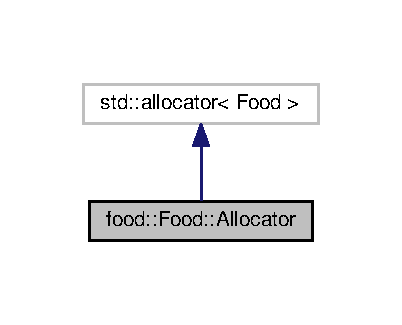
\includegraphics[width=193pt]{structfood_1_1_food_1_1_allocator__inherit__graph}
\end{center}
\end{figure}


Collaboration diagram for food\+:\+:Food\+:\+:Allocator\+:
\nopagebreak
\begin{figure}[H]
\begin{center}
\leavevmode
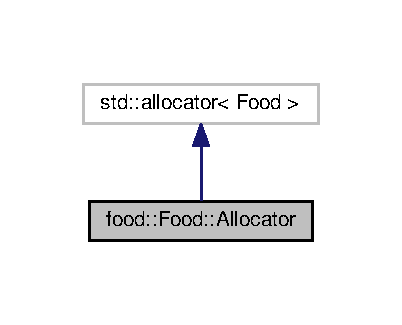
\includegraphics[width=193pt]{structfood_1_1_food_1_1_allocator__coll__graph}
\end{center}
\end{figure}
\subsection*{Classes}
\begin{DoxyCompactItemize}
\item 
struct \hyperlink{structfood_1_1_food_1_1_allocator_1_1rebind}{rebind}
\end{DoxyCompactItemize}
\subsection*{Public Member Functions}
\begin{DoxyCompactItemize}
\item 
{\footnotesize template$<$class Food , typename... Args$>$ }\\void \hyperlink{structfood_1_1_food_1_1_allocator_a1e2f18e58bb04189eaf7b56dccca818c}{construct} (\hyperlink{classfood_1_1_food}{Food} $\ast$buffer, Args \&\&...args)
\end{DoxyCompactItemize}


\subsection{Detailed Description}
Custom allocator that allows database utils to own a vector of storable objects with private constructors. 

\subsection{Member Function Documentation}
\index{food\+::\+Food\+::\+Allocator@{food\+::\+Food\+::\+Allocator}!construct@{construct}}
\index{construct@{construct}!food\+::\+Food\+::\+Allocator@{food\+::\+Food\+::\+Allocator}}
\subsubsection[{\texorpdfstring{construct(\+Food $\ast$buffer, Args \&\&...\+args)}{construct(Food *buffer, Args &&...args)}}]{\setlength{\rightskip}{0pt plus 5cm}template$<$class Food , typename... Args$>$ void food\+::\+Food\+::\+Allocator\+::construct (
\begin{DoxyParamCaption}
\item[{{\bf Food} $\ast$}]{buffer, }
\item[{Args \&\&...}]{args}
\end{DoxyParamCaption}
)\hspace{0.3cm}{\ttfamily [inline]}}\hypertarget{structfood_1_1_food_1_1_allocator_a1e2f18e58bb04189eaf7b56dccca818c}{}\label{structfood_1_1_food_1_1_allocator_a1e2f18e58bb04189eaf7b56dccca818c}
In place new construction of storable by memory pool that is given

The documentation for this struct was generated from the following file\+:\begin{DoxyCompactItemize}
\item 
/home/travis/build/\+Manuel\+Meraz/\+Tracker/include/food/\hyperlink{_food_8hpp}{Food.\+hpp}\end{DoxyCompactItemize}

\hypertarget{structfood_1_1_carbohydrate}{}\section{food\+:\+:Carbohydrate Struct Reference}
\label{structfood_1_1_carbohydrate}\index{food\+::\+Carbohydrate@{food\+::\+Carbohydrate}}


Stores the carbohydrate content of a food.  




{\ttfamily \#include $<$Macronutrients.\+hpp$>$}

\subsection*{Public Member Functions}
\begin{DoxyCompactItemize}
\item 
\hyperlink{structfood_1_1_carbohydrate_a21a8fd981abf8007d2b3f4d3eb516a49}{Carbohydrate} ()
\item 
\hyperlink{structfood_1_1_carbohydrate_a249b85edd7701182b4baac7b5b9d1973}{Carbohydrate} (double total\+\_\+carb)
\item 
\hyperlink{structfood_1_1_carbohydrate_af22de9314711f988826c8e7602472f65}{Carbohydrate} (double total\+\_\+carb, \hyperlink{structfood_1_1_fiber}{Fiber} const \&fiber)
\end{DoxyCompactItemize}
\subsection*{Public Attributes}
\begin{DoxyCompactItemize}
\item 
double \hyperlink{structfood_1_1_carbohydrate_a7f187c69c3f4a4013b2208c207b056dc}{quantity\+\_\+carb}
\begin{DoxyCompactList}\small\item\em The total carbohydrate in grams per 100g of food. \end{DoxyCompactList}\item 
double \hyperlink{structfood_1_1_carbohydrate_a6d66e644feb14e99eeba8e3b3c4b70ac}{quantity\+\_\+fiber}
\begin{DoxyCompactList}\small\item\em The total fiber in grams per 100g of food. \end{DoxyCompactList}\end{DoxyCompactItemize}


\subsection{Detailed Description}
Stores the carbohydrate content of a food. 

\subsection{Constructor \& Destructor Documentation}
\index{food\+::\+Carbohydrate@{food\+::\+Carbohydrate}!Carbohydrate@{Carbohydrate}}
\index{Carbohydrate@{Carbohydrate}!food\+::\+Carbohydrate@{food\+::\+Carbohydrate}}
\subsubsection[{\texorpdfstring{Carbohydrate()}{Carbohydrate()}}]{\setlength{\rightskip}{0pt plus 5cm}food\+::\+Carbohydrate\+::\+Carbohydrate (
\begin{DoxyParamCaption}
{}
\end{DoxyParamCaption}
)}\hypertarget{structfood_1_1_carbohydrate_a21a8fd981abf8007d2b3f4d3eb516a49}{}\label{structfood_1_1_carbohydrate_a21a8fd981abf8007d2b3f4d3eb516a49}
\index{food\+::\+Carbohydrate@{food\+::\+Carbohydrate}!Carbohydrate@{Carbohydrate}}
\index{Carbohydrate@{Carbohydrate}!food\+::\+Carbohydrate@{food\+::\+Carbohydrate}}
\subsubsection[{\texorpdfstring{Carbohydrate(double total\+\_\+carb)}{Carbohydrate(double total_carb)}}]{\setlength{\rightskip}{0pt plus 5cm}food\+::\+Carbohydrate\+::\+Carbohydrate (
\begin{DoxyParamCaption}
\item[{double}]{total\+\_\+carb}
\end{DoxyParamCaption}
)\hspace{0.3cm}{\ttfamily [explicit]}}\hypertarget{structfood_1_1_carbohydrate_a249b85edd7701182b4baac7b5b9d1973}{}\label{structfood_1_1_carbohydrate_a249b85edd7701182b4baac7b5b9d1973}

\begin{DoxyParams}{Parameters}
{\em total\+\_\+carb} & The total carbohydrate in grams per 100g of food \\
\hline
\end{DoxyParams}
\index{food\+::\+Carbohydrate@{food\+::\+Carbohydrate}!Carbohydrate@{Carbohydrate}}
\index{Carbohydrate@{Carbohydrate}!food\+::\+Carbohydrate@{food\+::\+Carbohydrate}}
\subsubsection[{\texorpdfstring{Carbohydrate(double total\+\_\+carb, Fiber const \&fiber)}{Carbohydrate(double total_carb, Fiber const &fiber)}}]{\setlength{\rightskip}{0pt plus 5cm}food\+::\+Carbohydrate\+::\+Carbohydrate (
\begin{DoxyParamCaption}
\item[{double}]{total\+\_\+carb, }
\item[{{\bf Fiber} const \&}]{fiber}
\end{DoxyParamCaption}
)\hspace{0.3cm}{\ttfamily [explicit]}}\hypertarget{structfood_1_1_carbohydrate_af22de9314711f988826c8e7602472f65}{}\label{structfood_1_1_carbohydrate_af22de9314711f988826c8e7602472f65}

\begin{DoxyParams}{Parameters}
{\em total\+\_\+carb} & The total carbohydrate in grams per 100g of food \\
\hline
{\em fiber} & The total fiber in grams per 100g of food \\
\hline
\end{DoxyParams}


\subsection{Member Data Documentation}
\index{food\+::\+Carbohydrate@{food\+::\+Carbohydrate}!quantity\+\_\+carb@{quantity\+\_\+carb}}
\index{quantity\+\_\+carb@{quantity\+\_\+carb}!food\+::\+Carbohydrate@{food\+::\+Carbohydrate}}
\subsubsection[{\texorpdfstring{quantity\+\_\+carb}{quantity_carb}}]{\setlength{\rightskip}{0pt plus 5cm}double food\+::\+Carbohydrate\+::quantity\+\_\+carb}\hypertarget{structfood_1_1_carbohydrate_a7f187c69c3f4a4013b2208c207b056dc}{}\label{structfood_1_1_carbohydrate_a7f187c69c3f4a4013b2208c207b056dc}


The total carbohydrate in grams per 100g of food. 

\index{food\+::\+Carbohydrate@{food\+::\+Carbohydrate}!quantity\+\_\+fiber@{quantity\+\_\+fiber}}
\index{quantity\+\_\+fiber@{quantity\+\_\+fiber}!food\+::\+Carbohydrate@{food\+::\+Carbohydrate}}
\subsubsection[{\texorpdfstring{quantity\+\_\+fiber}{quantity_fiber}}]{\setlength{\rightskip}{0pt plus 5cm}double food\+::\+Carbohydrate\+::quantity\+\_\+fiber}\hypertarget{structfood_1_1_carbohydrate_a6d66e644feb14e99eeba8e3b3c4b70ac}{}\label{structfood_1_1_carbohydrate_a6d66e644feb14e99eeba8e3b3c4b70ac}


The total fiber in grams per 100g of food. 



The documentation for this struct was generated from the following files\+:\begin{DoxyCompactItemize}
\item 
/home/travis/build/\+Manuel\+Meraz/\+Tracker/include/food/\hyperlink{_macronutrients_8hpp}{Macronutrients.\+hpp}\item 
/home/travis/build/\+Manuel\+Meraz/\+Tracker/src/food/\hyperlink{_macronutrients_8cpp}{Macronutrients.\+cpp}\end{DoxyCompactItemize}

\hypertarget{structdatabase_1_1_column_properties}{}\section{database\+:\+:Column\+Properties Struct Reference}
\label{structdatabase_1_1_column_properties}\index{database\+::\+Column\+Properties@{database\+::\+Column\+Properties}}


The column properties for a column in a table. A group of these represents a schema.  




{\ttfamily \#include $<$Data.\+hpp$>$}

\subsection*{Public Attributes}
\begin{DoxyCompactItemize}
\item 
std\+::string \hyperlink{structdatabase_1_1_column_properties_a69a1e887784799661e9345b0f4d88256}{name}
\begin{DoxyCompactList}\small\item\em The name of the column. \end{DoxyCompactList}\item 
\hyperlink{namespacedatabase_a596cea80c57ec5a9b3b4018f733a43fd}{Data\+Type} \hyperlink{structdatabase_1_1_column_properties_a34af986257f79a7b2c9ad2e01013f99e}{data\+\_\+type}
\begin{DoxyCompactList}\small\item\em The type of data to be stored in the database (e.\+g. R\+E\+AL, I\+N\+T\+E\+G\+ER, T\+E\+XT, etc) \end{DoxyCompactList}\item 
\hyperlink{namespacedatabase_a77defe1118948f64f1e32f4b78c04f5b}{Constraint} \hyperlink{structdatabase_1_1_column_properties_a587d4ebc4c0e8ebfa48e336a08f234f5}{constraint}
\begin{DoxyCompactList}\small\item\em The constraint of the data when creating the table (e.\+g. P\+R\+I\+M\+A\+RY K\+EY, U\+N\+I\+Q\+UE, N\+OT N\+U\+LL, or C\+H\+E\+CK). \end{DoxyCompactList}\end{DoxyCompactItemize}


\subsection{Detailed Description}
The column properties for a column in a table. A group of these represents a schema. 

\subsection{Member Data Documentation}
\index{database\+::\+Column\+Properties@{database\+::\+Column\+Properties}!constraint@{constraint}}
\index{constraint@{constraint}!database\+::\+Column\+Properties@{database\+::\+Column\+Properties}}
\subsubsection[{\texorpdfstring{constraint}{constraint}}]{\setlength{\rightskip}{0pt plus 5cm}{\bf Constraint} database\+::\+Column\+Properties\+::constraint}\hypertarget{structdatabase_1_1_column_properties_a587d4ebc4c0e8ebfa48e336a08f234f5}{}\label{structdatabase_1_1_column_properties_a587d4ebc4c0e8ebfa48e336a08f234f5}


The constraint of the data when creating the table (e.\+g. P\+R\+I\+M\+A\+RY K\+EY, U\+N\+I\+Q\+UE, N\+OT N\+U\+LL, or C\+H\+E\+CK). 

\index{database\+::\+Column\+Properties@{database\+::\+Column\+Properties}!data\+\_\+type@{data\+\_\+type}}
\index{data\+\_\+type@{data\+\_\+type}!database\+::\+Column\+Properties@{database\+::\+Column\+Properties}}
\subsubsection[{\texorpdfstring{data\+\_\+type}{data_type}}]{\setlength{\rightskip}{0pt plus 5cm}{\bf Data\+Type} database\+::\+Column\+Properties\+::data\+\_\+type}\hypertarget{structdatabase_1_1_column_properties_a34af986257f79a7b2c9ad2e01013f99e}{}\label{structdatabase_1_1_column_properties_a34af986257f79a7b2c9ad2e01013f99e}


The type of data to be stored in the database (e.\+g. R\+E\+AL, I\+N\+T\+E\+G\+ER, T\+E\+XT, etc) 

\index{database\+::\+Column\+Properties@{database\+::\+Column\+Properties}!name@{name}}
\index{name@{name}!database\+::\+Column\+Properties@{database\+::\+Column\+Properties}}
\subsubsection[{\texorpdfstring{name}{name}}]{\setlength{\rightskip}{0pt plus 5cm}std\+::string database\+::\+Column\+Properties\+::name}\hypertarget{structdatabase_1_1_column_properties_a69a1e887784799661e9345b0f4d88256}{}\label{structdatabase_1_1_column_properties_a69a1e887784799661e9345b0f4d88256}


The name of the column. 



The documentation for this struct was generated from the following file\+:\begin{DoxyCompactItemize}
\item 
/home/travis/build/\+Manuel\+Meraz/\+Tracker/include/database/\hyperlink{_data_8hpp}{Data.\+hpp}\end{DoxyCompactItemize}

\hypertarget{structdatabase_1_1_data}{}\section{database\+:\+:Data Struct Reference}
\label{structdatabase_1_1_data}\index{database\+::\+Data@{database\+::\+Data}}


The data to be stored into a database.  




{\ttfamily \#include $<$Data.\+hpp$>$}

\subsection*{Public Attributes}
\begin{DoxyCompactItemize}
\item 
std\+::string \hyperlink{structdatabase_1_1_data_a1a24b475b6698376a166ff80ef0a8fe8}{table\+\_\+name}
\begin{DoxyCompactList}\small\item\em The table name where the data will be stored. \end{DoxyCompactList}\item 
std\+::vector$<$ \hyperlink{structdatabase_1_1_column_properties}{Column\+Properties} $>$ \hyperlink{structdatabase_1_1_data_ae674b19f66a2cdfafa134304121ebbe2}{schema}
\begin{DoxyCompactList}\small\item\em The schema of the table. \end{DoxyCompactList}\item 
std\+::vector$<$ \hyperlink{structdatabase_1_1_row}{Row} $>$ \hyperlink{structdatabase_1_1_data_ae45d84ed5b3ce80a7683df0c3f40d518}{rows}
\begin{DoxyCompactList}\small\item\em Each row contains the raw variant data in the same order as the schema. \end{DoxyCompactList}\end{DoxyCompactItemize}


\subsection{Detailed Description}
The data to be stored into a database. 

\subsection{Member Data Documentation}
\index{database\+::\+Data@{database\+::\+Data}!rows@{rows}}
\index{rows@{rows}!database\+::\+Data@{database\+::\+Data}}
\subsubsection[{\texorpdfstring{rows}{rows}}]{\setlength{\rightskip}{0pt plus 5cm}std\+::vector$<${\bf Row}$>$ database\+::\+Data\+::rows}\hypertarget{structdatabase_1_1_data_ae45d84ed5b3ce80a7683df0c3f40d518}{}\label{structdatabase_1_1_data_ae45d84ed5b3ce80a7683df0c3f40d518}


Each row contains the raw variant data in the same order as the schema. 

\index{database\+::\+Data@{database\+::\+Data}!schema@{schema}}
\index{schema@{schema}!database\+::\+Data@{database\+::\+Data}}
\subsubsection[{\texorpdfstring{schema}{schema}}]{\setlength{\rightskip}{0pt plus 5cm}std\+::vector$<${\bf Column\+Properties}$>$ database\+::\+Data\+::schema}\hypertarget{structdatabase_1_1_data_ae674b19f66a2cdfafa134304121ebbe2}{}\label{structdatabase_1_1_data_ae674b19f66a2cdfafa134304121ebbe2}


The schema of the table. 

\index{database\+::\+Data@{database\+::\+Data}!table\+\_\+name@{table\+\_\+name}}
\index{table\+\_\+name@{table\+\_\+name}!database\+::\+Data@{database\+::\+Data}}
\subsubsection[{\texorpdfstring{table\+\_\+name}{table_name}}]{\setlength{\rightskip}{0pt plus 5cm}std\+::string database\+::\+Data\+::table\+\_\+name}\hypertarget{structdatabase_1_1_data_a1a24b475b6698376a166ff80ef0a8fe8}{}\label{structdatabase_1_1_data_a1a24b475b6698376a166ff80ef0a8fe8}


The table name where the data will be stored. 



The documentation for this struct was generated from the following file\+:\begin{DoxyCompactItemize}
\item 
/home/travis/build/\+Manuel\+Meraz/\+Tracker/include/database/\hyperlink{_data_8hpp}{Data.\+hpp}\end{DoxyCompactItemize}

\hypertarget{classdatabase_1_1_database}{}\section{database\+:\+:Database Class Reference}
\label{classdatabase_1_1_database}\index{database\+::\+Database@{database\+::\+Database}}


The database singleton class is in charge all database queries.  




{\ttfamily \#include $<$Database.\+hpp$>$}

\subsection*{Public Member Functions}
\begin{DoxyCompactItemize}
\item 
\hyperlink{classdatabase_1_1_database_af32a0bd3a5a492d478a215ef50f6ed14}{Database} (const \hyperlink{classdatabase_1_1_database}{Database} \&)=delete
\begin{DoxyCompactList}\small\item\em Deleted functions. \end{DoxyCompactList}\item 
\hyperlink{classdatabase_1_1_database_af23c97c26b274d8d32eaa9c7af5ee8f4}{Database} (\hyperlink{classdatabase_1_1_database}{Database} \&\&)=delete
\item 
\hyperlink{classdatabase_1_1_database}{Database} \& \hyperlink{classdatabase_1_1_database_afb30d33ce289a82f9f41ac59df63ec68}{operator=} (const \hyperlink{classdatabase_1_1_database}{Database} \&)=delete
\item 
\hyperlink{classdatabase_1_1_database}{Database} \& \hyperlink{classdatabase_1_1_database_a6652af8e150bdc26c786869efde743c0}{operator=} (\hyperlink{classdatabase_1_1_database}{Database} \&\&)=delete
\end{DoxyCompactItemize}
\subsection*{Static Public Member Functions}
\begin{DoxyCompactItemize}
\item 
static auto \hyperlink{classdatabase_1_1_database_a9de5cff42e2434006824d5f98a1e7492}{get\+\_\+connection} () -\/$>$ soci\+::session \&
\begin{DoxyCompactList}\small\item\em Returns a reference to the current database connection;. \end{DoxyCompactList}\end{DoxyCompactItemize}


\subsection{Detailed Description}
The database singleton class is in charge all database queries. 

Due to the way S\+Q\+Lite works, we want a single connection to the database up and running at all times. This class keeps the connection maintained. 

\subsection{Constructor \& Destructor Documentation}
\index{database\+::\+Database@{database\+::\+Database}!Database@{Database}}
\index{Database@{Database}!database\+::\+Database@{database\+::\+Database}}
\subsubsection[{\texorpdfstring{Database(const Database \&)=delete}{Database(const Database &)=delete}}]{\setlength{\rightskip}{0pt plus 5cm}database\+::\+Database\+::\+Database (
\begin{DoxyParamCaption}
\item[{const {\bf Database} \&}]{}
\end{DoxyParamCaption}
)\hspace{0.3cm}{\ttfamily [delete]}}\hypertarget{classdatabase_1_1_database_af32a0bd3a5a492d478a215ef50f6ed14}{}\label{classdatabase_1_1_database_af32a0bd3a5a492d478a215ef50f6ed14}


Deleted functions. 

\index{database\+::\+Database@{database\+::\+Database}!Database@{Database}}
\index{Database@{Database}!database\+::\+Database@{database\+::\+Database}}
\subsubsection[{\texorpdfstring{Database(\+Database \&\&)=delete}{Database(Database &&)=delete}}]{\setlength{\rightskip}{0pt plus 5cm}database\+::\+Database\+::\+Database (
\begin{DoxyParamCaption}
\item[{{\bf Database} \&\&}]{}
\end{DoxyParamCaption}
)\hspace{0.3cm}{\ttfamily [delete]}}\hypertarget{classdatabase_1_1_database_af23c97c26b274d8d32eaa9c7af5ee8f4}{}\label{classdatabase_1_1_database_af23c97c26b274d8d32eaa9c7af5ee8f4}


\subsection{Member Function Documentation}
\index{database\+::\+Database@{database\+::\+Database}!get\+\_\+connection@{get\+\_\+connection}}
\index{get\+\_\+connection@{get\+\_\+connection}!database\+::\+Database@{database\+::\+Database}}
\subsubsection[{\texorpdfstring{get\+\_\+connection() -\/$>$ soci\+::session \&}{get_connection() -> soci::session &}}]{\setlength{\rightskip}{0pt plus 5cm}auto database\+::\+Database\+::get\+\_\+connection (
\begin{DoxyParamCaption}
{}
\end{DoxyParamCaption}
) -\/$>$ soci\+::session \&\hspace{0.3cm}{\ttfamily [static]}}\hypertarget{classdatabase_1_1_database_a9de5cff42e2434006824d5f98a1e7492}{}\label{classdatabase_1_1_database_a9de5cff42e2434006824d5f98a1e7492}


Returns a reference to the current database connection;. 

Need to return a reference explicitly because this item is uncopyable. Attempts to copy the connection will try to call a private constructor and fail.

Usage\+: ~\newline
 auto\& sql\+\_\+connection = \hyperlink{classdatabase_1_1_database_a9de5cff42e2434006824d5f98a1e7492}{database\+::\+Database\+::get\+\_\+connection()}; ~\newline
 sql\+\_\+connection $<$$<$ \char`\"{}some sql command here\char`\"{};

Will throw a soci\+::sqlite3\+\_\+soci\+\_\+error if the command fails \index{database\+::\+Database@{database\+::\+Database}!operator=@{operator=}}
\index{operator=@{operator=}!database\+::\+Database@{database\+::\+Database}}
\subsubsection[{\texorpdfstring{operator=(const Database \&)=delete}{operator=(const Database &)=delete}}]{\setlength{\rightskip}{0pt plus 5cm}{\bf Database}\& database\+::\+Database\+::operator= (
\begin{DoxyParamCaption}
\item[{const {\bf Database} \&}]{}
\end{DoxyParamCaption}
)\hspace{0.3cm}{\ttfamily [delete]}}\hypertarget{classdatabase_1_1_database_afb30d33ce289a82f9f41ac59df63ec68}{}\label{classdatabase_1_1_database_afb30d33ce289a82f9f41ac59df63ec68}
\index{database\+::\+Database@{database\+::\+Database}!operator=@{operator=}}
\index{operator=@{operator=}!database\+::\+Database@{database\+::\+Database}}
\subsubsection[{\texorpdfstring{operator=(\+Database \&\&)=delete}{operator=(Database &&)=delete}}]{\setlength{\rightskip}{0pt plus 5cm}{\bf Database}\& database\+::\+Database\+::operator= (
\begin{DoxyParamCaption}
\item[{{\bf Database} \&\&}]{}
\end{DoxyParamCaption}
)\hspace{0.3cm}{\ttfamily [delete]}}\hypertarget{classdatabase_1_1_database_a6652af8e150bdc26c786869efde743c0}{}\label{classdatabase_1_1_database_a6652af8e150bdc26c786869efde743c0}


The documentation for this class was generated from the following files\+:\begin{DoxyCompactItemize}
\item 
/home/travis/build/\+Manuel\+Meraz/\+Tracker/include/database/\hyperlink{_database_8hpp}{Database.\+hpp}\item 
/home/travis/build/\+Manuel\+Meraz/\+Tracker/src/database/\hyperlink{_database_8cpp}{Database.\+cpp}\end{DoxyCompactItemize}

\hypertarget{structfood_1_1_fat}{}\section{food\+:\+:Fat Struct Reference}
\label{structfood_1_1_fat}\index{food\+::\+Fat@{food\+::\+Fat}}


Stores the fat content of a food.  




{\ttfamily \#include $<$Macronutrients.\+hpp$>$}

\subsection*{Public Member Functions}
\begin{DoxyCompactItemize}
\item 
\hyperlink{structfood_1_1_fat_ac3a105ffc2e83809f6f074d8d7ad7484}{Fat} ()
\item 
\hyperlink{structfood_1_1_fat_af32185aa0bb436f1dfdafe8e6f95d463}{Fat} (double \hyperlink{structfood_1_1_fat_a1cb066752937c4fbccd9e2a5ec4fa81b}{quantity})
\end{DoxyCompactItemize}
\subsection*{Public Attributes}
\begin{DoxyCompactItemize}
\item 
double \hyperlink{structfood_1_1_fat_a1cb066752937c4fbccd9e2a5ec4fa81b}{quantity}
\begin{DoxyCompactList}\small\item\em The quantiy of fat in grams per 100g of food. \end{DoxyCompactList}\end{DoxyCompactItemize}


\subsection{Detailed Description}
Stores the fat content of a food. 

\subsection{Constructor \& Destructor Documentation}
\index{food\+::\+Fat@{food\+::\+Fat}!Fat@{Fat}}
\index{Fat@{Fat}!food\+::\+Fat@{food\+::\+Fat}}
\subsubsection[{\texorpdfstring{Fat()}{Fat()}}]{\setlength{\rightskip}{0pt plus 5cm}food\+::\+Fat\+::\+Fat (
\begin{DoxyParamCaption}
{}
\end{DoxyParamCaption}
)}\hypertarget{structfood_1_1_fat_ac3a105ffc2e83809f6f074d8d7ad7484}{}\label{structfood_1_1_fat_ac3a105ffc2e83809f6f074d8d7ad7484}
\index{food\+::\+Fat@{food\+::\+Fat}!Fat@{Fat}}
\index{Fat@{Fat}!food\+::\+Fat@{food\+::\+Fat}}
\subsubsection[{\texorpdfstring{Fat(double quantity)}{Fat(double quantity)}}]{\setlength{\rightskip}{0pt plus 5cm}food\+::\+Fat\+::\+Fat (
\begin{DoxyParamCaption}
\item[{double}]{quantity}
\end{DoxyParamCaption}
)\hspace{0.3cm}{\ttfamily [explicit]}}\hypertarget{structfood_1_1_fat_af32185aa0bb436f1dfdafe8e6f95d463}{}\label{structfood_1_1_fat_af32185aa0bb436f1dfdafe8e6f95d463}

\begin{DoxyParams}{Parameters}
{\em quantity} & The quantiy of fat in grams per 100g of food \\
\hline
\end{DoxyParams}


\subsection{Member Data Documentation}
\index{food\+::\+Fat@{food\+::\+Fat}!quantity@{quantity}}
\index{quantity@{quantity}!food\+::\+Fat@{food\+::\+Fat}}
\subsubsection[{\texorpdfstring{quantity}{quantity}}]{\setlength{\rightskip}{0pt plus 5cm}double food\+::\+Fat\+::quantity}\hypertarget{structfood_1_1_fat_a1cb066752937c4fbccd9e2a5ec4fa81b}{}\label{structfood_1_1_fat_a1cb066752937c4fbccd9e2a5ec4fa81b}


The quantiy of fat in grams per 100g of food. 



The documentation for this struct was generated from the following files\+:\begin{DoxyCompactItemize}
\item 
/home/travis/build/\+Manuel\+Meraz/\+Tracker/include/food/\hyperlink{_macronutrients_8hpp}{Macronutrients.\+hpp}\item 
/home/travis/build/\+Manuel\+Meraz/\+Tracker/src/food/\hyperlink{_macronutrients_8cpp}{Macronutrients.\+cpp}\end{DoxyCompactItemize}

\hypertarget{structfood_1_1_fiber}{}\section{food\+:\+:Fiber Struct Reference}
\label{structfood_1_1_fiber}\index{food\+::\+Fiber@{food\+::\+Fiber}}


Stores the fiber content of a food.  




{\ttfamily \#include $<$Macronutrients.\+hpp$>$}

\subsection*{Public Member Functions}
\begin{DoxyCompactItemize}
\item 
\hyperlink{structfood_1_1_fiber_a8db0bd1ded433301bb0a26457bc427f3}{Fiber} ()
\item 
\hyperlink{structfood_1_1_fiber_a0b44bfb41f5e63369f42e5b8008d9d4e}{Fiber} (double \hyperlink{structfood_1_1_fiber_a08ab124e49a11cc8bde9a502c7e2fed1}{quantity})
\end{DoxyCompactItemize}
\subsection*{Public Attributes}
\begin{DoxyCompactItemize}
\item 
double \hyperlink{structfood_1_1_fiber_a08ab124e49a11cc8bde9a502c7e2fed1}{quantity}
\begin{DoxyCompactList}\small\item\em quantity The quantity of fiber in grams per 100g of food \end{DoxyCompactList}\end{DoxyCompactItemize}


\subsection{Detailed Description}
Stores the fiber content of a food. 

\subsection{Constructor \& Destructor Documentation}
\index{food\+::\+Fiber@{food\+::\+Fiber}!Fiber@{Fiber}}
\index{Fiber@{Fiber}!food\+::\+Fiber@{food\+::\+Fiber}}
\subsubsection[{\texorpdfstring{Fiber()}{Fiber()}}]{\setlength{\rightskip}{0pt plus 5cm}food\+::\+Fiber\+::\+Fiber (
\begin{DoxyParamCaption}
{}
\end{DoxyParamCaption}
)}\hypertarget{structfood_1_1_fiber_a8db0bd1ded433301bb0a26457bc427f3}{}\label{structfood_1_1_fiber_a8db0bd1ded433301bb0a26457bc427f3}
\index{food\+::\+Fiber@{food\+::\+Fiber}!Fiber@{Fiber}}
\index{Fiber@{Fiber}!food\+::\+Fiber@{food\+::\+Fiber}}
\subsubsection[{\texorpdfstring{Fiber(double quantity)}{Fiber(double quantity)}}]{\setlength{\rightskip}{0pt plus 5cm}food\+::\+Fiber\+::\+Fiber (
\begin{DoxyParamCaption}
\item[{double}]{quantity}
\end{DoxyParamCaption}
)\hspace{0.3cm}{\ttfamily [explicit]}}\hypertarget{structfood_1_1_fiber_a0b44bfb41f5e63369f42e5b8008d9d4e}{}\label{structfood_1_1_fiber_a0b44bfb41f5e63369f42e5b8008d9d4e}

\begin{DoxyParams}{Parameters}
{\em quantity} & The quantity of fiber in grams per 100g of food \\
\hline
\end{DoxyParams}


\subsection{Member Data Documentation}
\index{food\+::\+Fiber@{food\+::\+Fiber}!quantity@{quantity}}
\index{quantity@{quantity}!food\+::\+Fiber@{food\+::\+Fiber}}
\subsubsection[{\texorpdfstring{quantity}{quantity}}]{\setlength{\rightskip}{0pt plus 5cm}double food\+::\+Fiber\+::quantity}\hypertarget{structfood_1_1_fiber_a08ab124e49a11cc8bde9a502c7e2fed1}{}\label{structfood_1_1_fiber_a08ab124e49a11cc8bde9a502c7e2fed1}


quantity The quantity of fiber in grams per 100g of food 



The documentation for this struct was generated from the following files\+:\begin{DoxyCompactItemize}
\item 
/home/travis/build/\+Manuel\+Meraz/\+Tracker/include/food/\hyperlink{_macronutrients_8hpp}{Macronutrients.\+hpp}\item 
/home/travis/build/\+Manuel\+Meraz/\+Tracker/src/food/\hyperlink{_macronutrients_8cpp}{Macronutrients.\+cpp}\end{DoxyCompactItemize}

\hypertarget{classfood_1_1_food}{}\section{food\+:\+:Food Class Reference}
\label{classfood_1_1_food}\index{food\+::\+Food@{food\+::\+Food}}


The food class stores all macronutrient and micronutrient data for any food.  




{\ttfamily \#include $<$Food.\+hpp$>$}



Inheritance diagram for food\+:\+:Food\+:
\nopagebreak
\begin{figure}[H]
\begin{center}
\leavevmode
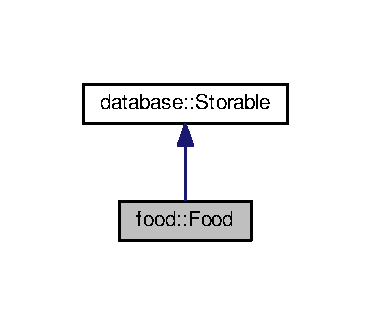
\includegraphics[width=178pt]{classfood_1_1_food__inherit__graph}
\end{center}
\end{figure}


Collaboration diagram for food\+:\+:Food\+:
\nopagebreak
\begin{figure}[H]
\begin{center}
\leavevmode
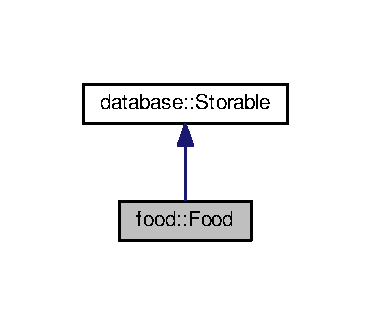
\includegraphics[width=178pt]{classfood_1_1_food__coll__graph}
\end{center}
\end{figure}
\subsection*{Classes}
\begin{DoxyCompactItemize}
\item 
struct \hyperlink{structfood_1_1_food_1_1_allocator}{Allocator}
\begin{DoxyCompactList}\small\item\em Custom allocator that allows database utils to own a vector of storable objects with private constructors. \end{DoxyCompactList}\end{DoxyCompactItemize}
\subsection*{Public Member Functions}
\begin{DoxyCompactItemize}
\item 
\hyperlink{classfood_1_1_food_ad3ba5861593fb753085ba502ca5d844a}{Food} (\hyperlink{classfood_1_1_food}{Food} \&\&f)=default
\item 
\hyperlink{classfood_1_1_food}{Food} \& \hyperlink{classfood_1_1_food_ae0ef42fe8425b35b39b1ea88e2dea27a}{operator=} (\hyperlink{classfood_1_1_food}{Food} const \&f)=default
\item 
\hyperlink{classfood_1_1_food}{Food} \& \hyperlink{classfood_1_1_food_a76b0691a40c6b412e04001af5a9af8e3}{operator=} (\hyperlink{classfood_1_1_food}{Food} \&\&f)=default
\item 
auto \hyperlink{classfood_1_1_food_ac3aefc08b78fa521b4317348463e5a5f}{get\+\_\+data} () const -\/$>$ \hyperlink{structdatabase_1_1_data}{database\+::\+Data} const override
\begin{DoxyCompactList}\small\item\em All data will be retrieved from a storable object using this function. \end{DoxyCompactList}\item 
auto \hyperlink{classfood_1_1_food_a76d21be86ff4500225e593205fc305c5}{id} () const -\/$>$ int override
\item 
auto \hyperlink{classfood_1_1_food_a29ccb0bdf6b74e6073b87bc71c70df04}{name} () const -\/$>$ std\+::string const override
\item 
void \hyperlink{classfood_1_1_food_ac717bda45254fd555b4de00004423041}{set\+\_\+name} (std\+::string\+\_\+view \hyperlink{classfood_1_1_food_a29ccb0bdf6b74e6073b87bc71c70df04}{name}) override
\item 
auto \hyperlink{classfood_1_1_food_a2ac3b444a1ef09dbcec63370f2c8f554}{str} () const -\/$>$ std\+::string override
\item 
auto \hyperlink{classfood_1_1_food_abea955fedfefd84254d7b788451a2a61}{macronutrients} () const -\/$>$ \hyperlink{classfood_1_1_macronutrients}{Macronutrients} const
\item 
void \hyperlink{classfood_1_1_food_a0df55be446b9dae80026bec62b2c1c5c}{set\+\_\+macronutrients} (\hyperlink{classfood_1_1_macronutrients}{Macronutrients} const \&macros)
\item 
\hyperlink{classfood_1_1_food_a065b75e0736ec60104419b9076db67c5}{$\sim$\+Food} () override=default
\end{DoxyCompactItemize}
\subsection*{Friends}
\begin{DoxyCompactItemize}
\item 
struct \hyperlink{classfood_1_1_food_ab18b852895cb6c78b137d008ac39d642}{Allocator}
\end{DoxyCompactItemize}


\subsection{Detailed Description}
The food class stores all macronutrient and micronutrient data for any food. 

\subsection{Constructor \& Destructor Documentation}
\index{food\+::\+Food@{food\+::\+Food}!Food@{Food}}
\index{Food@{Food}!food\+::\+Food@{food\+::\+Food}}
\subsubsection[{\texorpdfstring{Food(\+Food \&\&f)=default}{Food(Food &&f)=default}}]{\setlength{\rightskip}{0pt plus 5cm}food\+::\+Food\+::\+Food (
\begin{DoxyParamCaption}
\item[{{\bf Food} \&\&}]{f}
\end{DoxyParamCaption}
)\hspace{0.3cm}{\ttfamily [default]}}\hypertarget{classfood_1_1_food_ad3ba5861593fb753085ba502ca5d844a}{}\label{classfood_1_1_food_ad3ba5861593fb753085ba502ca5d844a}
\index{food\+::\+Food@{food\+::\+Food}!````~Food@{$\sim$\+Food}}
\index{````~Food@{$\sim$\+Food}!food\+::\+Food@{food\+::\+Food}}
\subsubsection[{\texorpdfstring{$\sim$\+Food() override=default}{~Food() override=default}}]{\setlength{\rightskip}{0pt plus 5cm}food\+::\+Food\+::$\sim$\+Food (
\begin{DoxyParamCaption}
{}
\end{DoxyParamCaption}
)\hspace{0.3cm}{\ttfamily [override]}, {\ttfamily [default]}}\hypertarget{classfood_1_1_food_a065b75e0736ec60104419b9076db67c5}{}\label{classfood_1_1_food_a065b75e0736ec60104419b9076db67c5}


\subsection{Member Function Documentation}
\index{food\+::\+Food@{food\+::\+Food}!get\+\_\+data@{get\+\_\+data}}
\index{get\+\_\+data@{get\+\_\+data}!food\+::\+Food@{food\+::\+Food}}
\subsubsection[{\texorpdfstring{get\+\_\+data() const -\/$>$ database\+::\+Data const override}{get_data() const -> database::Data const override}}]{\setlength{\rightskip}{0pt plus 5cm}auto food\+::\+Food\+::get\+\_\+data (
\begin{DoxyParamCaption}
{}
\end{DoxyParamCaption}
) const -\/$>$ {\bf database\+::\+Data} const\hspace{0.3cm}{\ttfamily [override]}, {\ttfamily [virtual]}}\hypertarget{classfood_1_1_food_ac3aefc08b78fa521b4317348463e5a5f}{}\label{classfood_1_1_food_ac3aefc08b78fa521b4317348463e5a5f}


All data will be retrieved from a storable object using this function. 

\begin{DoxyReturn}{Returns}
A struct containing the name of the table to store this data and a vector of column info. See \hyperlink{_data_8hpp}{Data.\+hpp} for more info. 
\end{DoxyReturn}


Implements \hyperlink{classdatabase_1_1_storable_afb1b1572e1147943227794f8abc0d0b0}{database\+::\+Storable}.

\index{food\+::\+Food@{food\+::\+Food}!id@{id}}
\index{id@{id}!food\+::\+Food@{food\+::\+Food}}
\subsubsection[{\texorpdfstring{id() const -\/$>$ int override}{id() const -> int override}}]{\setlength{\rightskip}{0pt plus 5cm}auto food\+::\+Food\+::id (
\begin{DoxyParamCaption}
{}
\end{DoxyParamCaption}
) const -\/$>$ int\hspace{0.3cm}{\ttfamily [override]}, {\ttfamily [virtual]}}\hypertarget{classfood_1_1_food_a76d21be86ff4500225e593205fc305c5}{}\label{classfood_1_1_food_a76d21be86ff4500225e593205fc305c5}
\begin{DoxyReturn}{Returns}
The unique ID of this food in the database 
\end{DoxyReturn}


Implements \hyperlink{classdatabase_1_1_storable_aafaf8ff3b7a854488ae6d4ab3e39f2af}{database\+::\+Storable}.

\index{food\+::\+Food@{food\+::\+Food}!macronutrients@{macronutrients}}
\index{macronutrients@{macronutrients}!food\+::\+Food@{food\+::\+Food}}
\subsubsection[{\texorpdfstring{macronutrients() const -\/$>$ Macronutrients const}{macronutrients() const -> Macronutrients const}}]{\setlength{\rightskip}{0pt plus 5cm}auto food\+::\+Food\+::macronutrients (
\begin{DoxyParamCaption}
{}
\end{DoxyParamCaption}
) const -\/$>$ {\bf Macronutrients} const}\hypertarget{classfood_1_1_food_abea955fedfefd84254d7b788451a2a61}{}\label{classfood_1_1_food_abea955fedfefd84254d7b788451a2a61}
\begin{DoxyReturn}{Returns}
The macronutrients of the food 
\end{DoxyReturn}
\index{food\+::\+Food@{food\+::\+Food}!name@{name}}
\index{name@{name}!food\+::\+Food@{food\+::\+Food}}
\subsubsection[{\texorpdfstring{name() const -\/$>$ std\+::string const override}{name() const -> std::string const override}}]{\setlength{\rightskip}{0pt plus 5cm}auto food\+::\+Food\+::name (
\begin{DoxyParamCaption}
{}
\end{DoxyParamCaption}
) const -\/$>$ std\+::string const\hspace{0.3cm}{\ttfamily [override]}, {\ttfamily [virtual]}}\hypertarget{classfood_1_1_food_a29ccb0bdf6b74e6073b87bc71c70df04}{}\label{classfood_1_1_food_a29ccb0bdf6b74e6073b87bc71c70df04}
\begin{DoxyReturn}{Returns}
The name of the food 
\end{DoxyReturn}


Implements \hyperlink{classdatabase_1_1_storable_a404fc104e41b9f1e52090a817c7d317e}{database\+::\+Storable}.

\index{food\+::\+Food@{food\+::\+Food}!operator=@{operator=}}
\index{operator=@{operator=}!food\+::\+Food@{food\+::\+Food}}
\subsubsection[{\texorpdfstring{operator=(\+Food const \&f)=default}{operator=(Food const &f)=default}}]{\setlength{\rightskip}{0pt plus 5cm}{\bf Food}\& food\+::\+Food\+::operator= (
\begin{DoxyParamCaption}
\item[{{\bf Food} const \&}]{f}
\end{DoxyParamCaption}
)\hspace{0.3cm}{\ttfamily [default]}}\hypertarget{classfood_1_1_food_ae0ef42fe8425b35b39b1ea88e2dea27a}{}\label{classfood_1_1_food_ae0ef42fe8425b35b39b1ea88e2dea27a}
\index{food\+::\+Food@{food\+::\+Food}!operator=@{operator=}}
\index{operator=@{operator=}!food\+::\+Food@{food\+::\+Food}}
\subsubsection[{\texorpdfstring{operator=(\+Food \&\&f)=default}{operator=(Food &&f)=default}}]{\setlength{\rightskip}{0pt plus 5cm}{\bf Food}\& food\+::\+Food\+::operator= (
\begin{DoxyParamCaption}
\item[{{\bf Food} \&\&}]{f}
\end{DoxyParamCaption}
)\hspace{0.3cm}{\ttfamily [default]}}\hypertarget{classfood_1_1_food_a76b0691a40c6b412e04001af5a9af8e3}{}\label{classfood_1_1_food_a76b0691a40c6b412e04001af5a9af8e3}
\index{food\+::\+Food@{food\+::\+Food}!set\+\_\+macronutrients@{set\+\_\+macronutrients}}
\index{set\+\_\+macronutrients@{set\+\_\+macronutrients}!food\+::\+Food@{food\+::\+Food}}
\subsubsection[{\texorpdfstring{set\+\_\+macronutrients(\+Macronutrients const \&macros)}{set_macronutrients(Macronutrients const &macros)}}]{\setlength{\rightskip}{0pt plus 5cm}void food\+::\+Food\+::set\+\_\+macronutrients (
\begin{DoxyParamCaption}
\item[{{\bf Macronutrients} const \&}]{macros}
\end{DoxyParamCaption}
)}\hypertarget{classfood_1_1_food_a0df55be446b9dae80026bec62b2c1c5c}{}\label{classfood_1_1_food_a0df55be446b9dae80026bec62b2c1c5c}
\begin{DoxyReturn}{Returns}
The macronutrients of the food 
\end{DoxyReturn}
\index{food\+::\+Food@{food\+::\+Food}!set\+\_\+name@{set\+\_\+name}}
\index{set\+\_\+name@{set\+\_\+name}!food\+::\+Food@{food\+::\+Food}}
\subsubsection[{\texorpdfstring{set\+\_\+name(std\+::string\+\_\+view name) override}{set_name(std::string_view name) override}}]{\setlength{\rightskip}{0pt plus 5cm}void food\+::\+Food\+::set\+\_\+name (
\begin{DoxyParamCaption}
\item[{std\+::string\+\_\+view}]{name}
\end{DoxyParamCaption}
)\hspace{0.3cm}{\ttfamily [override]}, {\ttfamily [virtual]}}\hypertarget{classfood_1_1_food_ac717bda45254fd555b4de00004423041}{}\label{classfood_1_1_food_ac717bda45254fd555b4de00004423041}
\begin{DoxyReturn}{Returns}
The name of the food 
\end{DoxyReturn}


Implements \hyperlink{classdatabase_1_1_storable_afa3a3acb030d9e33064c2f6e34f8bbcf}{database\+::\+Storable}.

\index{food\+::\+Food@{food\+::\+Food}!str@{str}}
\index{str@{str}!food\+::\+Food@{food\+::\+Food}}
\subsubsection[{\texorpdfstring{str() const -\/$>$ std\+::string override}{str() const -> std::string override}}]{\setlength{\rightskip}{0pt plus 5cm}auto food\+::\+Food\+::str (
\begin{DoxyParamCaption}
{}
\end{DoxyParamCaption}
) const -\/$>$ std\+::string\hspace{0.3cm}{\ttfamily [override]}, {\ttfamily [virtual]}}\hypertarget{classfood_1_1_food_a2ac3b444a1ef09dbcec63370f2c8f554}{}\label{classfood_1_1_food_a2ac3b444a1ef09dbcec63370f2c8f554}
\begin{DoxyReturn}{Returns}
string representation of the name and data, the same way sqlite displays table data 
\end{DoxyReturn}


Implements \hyperlink{classdatabase_1_1_storable_a3502dee26cdad8b8e3b0bf1ebc619dc4}{database\+::\+Storable}.



\subsection{Friends And Related Function Documentation}
\index{food\+::\+Food@{food\+::\+Food}!Allocator@{Allocator}}
\index{Allocator@{Allocator}!food\+::\+Food@{food\+::\+Food}}
\subsubsection[{\texorpdfstring{Allocator}{Allocator}}]{\setlength{\rightskip}{0pt plus 5cm}friend struct {\bf Allocator}\hspace{0.3cm}{\ttfamily [friend]}}\hypertarget{classfood_1_1_food_ab18b852895cb6c78b137d008ac39d642}{}\label{classfood_1_1_food_ab18b852895cb6c78b137d008ac39d642}


The documentation for this class was generated from the following files\+:\begin{DoxyCompactItemize}
\item 
/home/travis/build/\+Manuel\+Meraz/\+Tracker/include/food/\hyperlink{_food_8hpp}{Food.\+hpp}\item 
/home/travis/build/\+Manuel\+Meraz/\+Tracker/src/food/\hyperlink{_food_8cpp}{Food.\+cpp}\end{DoxyCompactItemize}

\hypertarget{classfood_1_1_macronutrients}{}\section{food\+:\+:Macronutrients Class Reference}
\label{classfood_1_1_macronutrients}\index{food\+::\+Macronutrients@{food\+::\+Macronutrients}}


The macronutrients class stores all macronutrient data to be stored in a \hyperlink{classfood_1_1_food}{Food} object.  




{\ttfamily \#include $<$Macronutrients.\+hpp$>$}

\subsection*{Public Member Functions}
\begin{DoxyCompactItemize}
\item 
\hyperlink{classfood_1_1_macronutrients_a41f7d2c1979da282b67824493d0905a6}{Macronutrients} ()
\item 
\hyperlink{classfood_1_1_macronutrients_afcb1c5e5380fbf25d1d0f9d3de17b335}{Macronutrients} (\hyperlink{structfood_1_1_fat}{Fat} const \&\hyperlink{classfood_1_1_macronutrients_aaf5c0f28fd6e7883c1536b44a415bb37}{fat}, \hyperlink{structfood_1_1_carbohydrate}{Carbohydrate} const \&carb, \hyperlink{structfood_1_1_protein}{Protein} const \&\hyperlink{classfood_1_1_macronutrients_a15a4120772455818fd7c088b99a2fae4}{protein})
\begin{DoxyCompactList}\small\item\em The classes passed in to this class are strongly typed classes to help illustrate the data being passed in. \end{DoxyCompactList}\item 
\hyperlink{classfood_1_1_macronutrients_adb6aeeac945e8dbd94734e967a6efc31}{Macronutrients} (\hyperlink{classfood_1_1_macronutrients}{Macronutrients} const \&macros)=default
\begin{DoxyCompactList}\small\item\em Copy constructor for lvalues reference. \end{DoxyCompactList}\item 
\hyperlink{classfood_1_1_macronutrients_af206f675652b58baa694078f9ad6ac27}{Macronutrients} (\hyperlink{classfood_1_1_macronutrients}{Macronutrients} \&\&macros) noexcept=default
\begin{DoxyCompactList}\small\item\em Move constructor for rvalue reference. \end{DoxyCompactList}\item 
\hyperlink{classfood_1_1_macronutrients}{Macronutrients} \& \hyperlink{classfood_1_1_macronutrients_a1da73b21a418ab85e806fdd83ec16316}{operator=} (\hyperlink{classfood_1_1_macronutrients}{Macronutrients} const \&macros)=default
\item 
\hyperlink{classfood_1_1_macronutrients}{Macronutrients} \& \hyperlink{classfood_1_1_macronutrients_a7c38fa08bff5787139cac7561cd902fd}{operator=} (\hyperlink{classfood_1_1_macronutrients}{Macronutrients} \&\&macros) noexcept=default
\begin{DoxyCompactList}\small\item\em Move assignment operator. \end{DoxyCompactList}\item 
auto \hyperlink{classfood_1_1_macronutrients_aaf5c0f28fd6e7883c1536b44a415bb37}{fat} () const -\/$>$ double
\item 
void \hyperlink{classfood_1_1_macronutrients_ab8c80226ba0243279d1c9852de4af504}{set\+\_\+fat} (double \hyperlink{classfood_1_1_macronutrients_aaf5c0f28fd6e7883c1536b44a415bb37}{fat})
\item 
auto \hyperlink{classfood_1_1_macronutrients_a40c64d630c1d964e858afe34ab313b8d}{carbohydrate} () const -\/$>$ double
\item 
void \hyperlink{classfood_1_1_macronutrients_a6c91ea66ab1bf9a67dfa63e46a8faf15}{set\+\_\+carbohydrate} (double \hyperlink{classfood_1_1_macronutrients_a40c64d630c1d964e858afe34ab313b8d}{carbohydrate})
\item 
auto \hyperlink{classfood_1_1_macronutrients_a623291db656bdfc2adc4f5e87d60e94a}{fiber} () const -\/$>$ double
\item 
void \hyperlink{classfood_1_1_macronutrients_a0a4c0bf9c8a75b985cab2770bb697169}{set\+\_\+fiber} (double \hyperlink{classfood_1_1_macronutrients_a623291db656bdfc2adc4f5e87d60e94a}{fiber})
\item 
auto \hyperlink{classfood_1_1_macronutrients_a15a4120772455818fd7c088b99a2fae4}{protein} () const -\/$>$ double
\item 
void \hyperlink{classfood_1_1_macronutrients_ae6c68d50351573c91105d59a23cab169}{set\+\_\+protein} (double \hyperlink{classfood_1_1_macronutrients_a15a4120772455818fd7c088b99a2fae4}{protein})
\item 
\hyperlink{classfood_1_1_macronutrients_aadc0948970a2105fcf53dbcc731a0697}{$\sim$\+Macronutrients} ()=default
\end{DoxyCompactItemize}


\subsection{Detailed Description}
The macronutrients class stores all macronutrient data to be stored in a \hyperlink{classfood_1_1_food}{Food} object. 

\subsection{Constructor \& Destructor Documentation}
\index{food\+::\+Macronutrients@{food\+::\+Macronutrients}!Macronutrients@{Macronutrients}}
\index{Macronutrients@{Macronutrients}!food\+::\+Macronutrients@{food\+::\+Macronutrients}}
\subsubsection[{\texorpdfstring{Macronutrients()}{Macronutrients()}}]{\setlength{\rightskip}{0pt plus 5cm}food\+::\+Macronutrients\+::\+Macronutrients (
\begin{DoxyParamCaption}
{}
\end{DoxyParamCaption}
)}\hypertarget{classfood_1_1_macronutrients_a41f7d2c1979da282b67824493d0905a6}{}\label{classfood_1_1_macronutrients_a41f7d2c1979da282b67824493d0905a6}
\index{food\+::\+Macronutrients@{food\+::\+Macronutrients}!Macronutrients@{Macronutrients}}
\index{Macronutrients@{Macronutrients}!food\+::\+Macronutrients@{food\+::\+Macronutrients}}
\subsubsection[{\texorpdfstring{Macronutrients(\+Fat const \&fat, Carbohydrate const \&carb, Protein const \&protein)}{Macronutrients(Fat const &fat, Carbohydrate const &carb, Protein const &protein)}}]{\setlength{\rightskip}{0pt plus 5cm}food\+::\+Macronutrients\+::\+Macronutrients (
\begin{DoxyParamCaption}
\item[{{\bf Fat} const \&}]{fat, }
\item[{{\bf Carbohydrate} const \&}]{carb, }
\item[{{\bf Protein} const \&}]{protein}
\end{DoxyParamCaption}
)}\hypertarget{classfood_1_1_macronutrients_afcb1c5e5380fbf25d1d0f9d3de17b335}{}\label{classfood_1_1_macronutrients_afcb1c5e5380fbf25d1d0f9d3de17b335}


The classes passed in to this class are strongly typed classes to help illustrate the data being passed in. 

The classes passed in to this class are strongly typed classes to help illustrate the data being passed in. All data passed in is in gramss per 100g of the food


\begin{DoxyParams}{Parameters}
{\em fat} & The fat content of the food \\
\hline
{\em carb} & The carbohydrate content of the food. Pass by value. \\
\hline
{\em protein} & The protein content of the food \\
\hline
\end{DoxyParams}
\index{food\+::\+Macronutrients@{food\+::\+Macronutrients}!Macronutrients@{Macronutrients}}
\index{Macronutrients@{Macronutrients}!food\+::\+Macronutrients@{food\+::\+Macronutrients}}
\subsubsection[{\texorpdfstring{Macronutrients(\+Macronutrients const \&macros)=default}{Macronutrients(Macronutrients const &macros)=default}}]{\setlength{\rightskip}{0pt plus 5cm}food\+::\+Macronutrients\+::\+Macronutrients (
\begin{DoxyParamCaption}
\item[{{\bf Macronutrients} const \&}]{macros}
\end{DoxyParamCaption}
)\hspace{0.3cm}{\ttfamily [default]}}\hypertarget{classfood_1_1_macronutrients_adb6aeeac945e8dbd94734e967a6efc31}{}\label{classfood_1_1_macronutrients_adb6aeeac945e8dbd94734e967a6efc31}


Copy constructor for lvalues reference. 


\begin{DoxyParams}{Parameters}
{\em macros} & The macros to be copied \\
\hline
\end{DoxyParams}
\index{food\+::\+Macronutrients@{food\+::\+Macronutrients}!Macronutrients@{Macronutrients}}
\index{Macronutrients@{Macronutrients}!food\+::\+Macronutrients@{food\+::\+Macronutrients}}
\subsubsection[{\texorpdfstring{Macronutrients(\+Macronutrients \&\&macros) noexcept=default}{Macronutrients(Macronutrients &&macros) noexcept=default}}]{\setlength{\rightskip}{0pt plus 5cm}food\+::\+Macronutrients\+::\+Macronutrients (
\begin{DoxyParamCaption}
\item[{{\bf Macronutrients} \&\&}]{macros}
\end{DoxyParamCaption}
)\hspace{0.3cm}{\ttfamily [default]}, {\ttfamily [noexcept]}}\hypertarget{classfood_1_1_macronutrients_af206f675652b58baa694078f9ad6ac27}{}\label{classfood_1_1_macronutrients_af206f675652b58baa694078f9ad6ac27}


Move constructor for rvalue reference. 


\begin{DoxyParams}{Parameters}
{\em macros} & The macros to be moved \\
\hline
\end{DoxyParams}
\index{food\+::\+Macronutrients@{food\+::\+Macronutrients}!````~Macronutrients@{$\sim$\+Macronutrients}}
\index{````~Macronutrients@{$\sim$\+Macronutrients}!food\+::\+Macronutrients@{food\+::\+Macronutrients}}
\subsubsection[{\texorpdfstring{$\sim$\+Macronutrients()=default}{~Macronutrients()=default}}]{\setlength{\rightskip}{0pt plus 5cm}food\+::\+Macronutrients\+::$\sim$\+Macronutrients (
\begin{DoxyParamCaption}
{}
\end{DoxyParamCaption}
)\hspace{0.3cm}{\ttfamily [default]}}\hypertarget{classfood_1_1_macronutrients_aadc0948970a2105fcf53dbcc731a0697}{}\label{classfood_1_1_macronutrients_aadc0948970a2105fcf53dbcc731a0697}


\subsection{Member Function Documentation}
\index{food\+::\+Macronutrients@{food\+::\+Macronutrients}!carbohydrate@{carbohydrate}}
\index{carbohydrate@{carbohydrate}!food\+::\+Macronutrients@{food\+::\+Macronutrients}}
\subsubsection[{\texorpdfstring{carbohydrate() const -\/$>$ double}{carbohydrate() const -> double}}]{\setlength{\rightskip}{0pt plus 5cm}auto food\+::\+Macronutrients\+::carbohydrate (
\begin{DoxyParamCaption}
{}
\end{DoxyParamCaption}
) const -\/$>$ double}\hypertarget{classfood_1_1_macronutrients_a40c64d630c1d964e858afe34ab313b8d}{}\label{classfood_1_1_macronutrients_a40c64d630c1d964e858afe34ab313b8d}
\begin{DoxyReturn}{Returns}
The quantity of carbohydrate 
\end{DoxyReturn}
\index{food\+::\+Macronutrients@{food\+::\+Macronutrients}!fat@{fat}}
\index{fat@{fat}!food\+::\+Macronutrients@{food\+::\+Macronutrients}}
\subsubsection[{\texorpdfstring{fat() const -\/$>$ double}{fat() const -> double}}]{\setlength{\rightskip}{0pt plus 5cm}auto food\+::\+Macronutrients\+::fat (
\begin{DoxyParamCaption}
{}
\end{DoxyParamCaption}
) const -\/$>$ double}\hypertarget{classfood_1_1_macronutrients_aaf5c0f28fd6e7883c1536b44a415bb37}{}\label{classfood_1_1_macronutrients_aaf5c0f28fd6e7883c1536b44a415bb37}
\begin{DoxyReturn}{Returns}
The quantity of fat 
\end{DoxyReturn}
\index{food\+::\+Macronutrients@{food\+::\+Macronutrients}!fiber@{fiber}}
\index{fiber@{fiber}!food\+::\+Macronutrients@{food\+::\+Macronutrients}}
\subsubsection[{\texorpdfstring{fiber() const -\/$>$ double}{fiber() const -> double}}]{\setlength{\rightskip}{0pt plus 5cm}auto food\+::\+Macronutrients\+::fiber (
\begin{DoxyParamCaption}
{}
\end{DoxyParamCaption}
) const -\/$>$ double}\hypertarget{classfood_1_1_macronutrients_a623291db656bdfc2adc4f5e87d60e94a}{}\label{classfood_1_1_macronutrients_a623291db656bdfc2adc4f5e87d60e94a}
\begin{DoxyReturn}{Returns}
The quantity of fiber 
\end{DoxyReturn}
\index{food\+::\+Macronutrients@{food\+::\+Macronutrients}!operator=@{operator=}}
\index{operator=@{operator=}!food\+::\+Macronutrients@{food\+::\+Macronutrients}}
\subsubsection[{\texorpdfstring{operator=(\+Macronutrients const \&macros)=default}{operator=(Macronutrients const &macros)=default}}]{\setlength{\rightskip}{0pt plus 5cm}{\bf Macronutrients}\& food\+::\+Macronutrients\+::operator= (
\begin{DoxyParamCaption}
\item[{{\bf Macronutrients} const \&}]{macros}
\end{DoxyParamCaption}
)\hspace{0.3cm}{\ttfamily [default]}}\hypertarget{classfood_1_1_macronutrients_a1da73b21a418ab85e806fdd83ec16316}{}\label{classfood_1_1_macronutrients_a1da73b21a418ab85e806fdd83ec16316}
Copy assignment operator 
\begin{DoxyParams}{Parameters}
{\em macros} & The macros to be copied \\
\hline
\end{DoxyParams}
\index{food\+::\+Macronutrients@{food\+::\+Macronutrients}!operator=@{operator=}}
\index{operator=@{operator=}!food\+::\+Macronutrients@{food\+::\+Macronutrients}}
\subsubsection[{\texorpdfstring{operator=(\+Macronutrients \&\&macros) noexcept=default}{operator=(Macronutrients &&macros) noexcept=default}}]{\setlength{\rightskip}{0pt plus 5cm}{\bf Macronutrients}\& food\+::\+Macronutrients\+::operator= (
\begin{DoxyParamCaption}
\item[{{\bf Macronutrients} \&\&}]{macros}
\end{DoxyParamCaption}
)\hspace{0.3cm}{\ttfamily [default]}, {\ttfamily [noexcept]}}\hypertarget{classfood_1_1_macronutrients_a7c38fa08bff5787139cac7561cd902fd}{}\label{classfood_1_1_macronutrients_a7c38fa08bff5787139cac7561cd902fd}


Move assignment operator. 


\begin{DoxyParams}{Parameters}
{\em macros} & The macros to be moved \\
\hline
\end{DoxyParams}
\index{food\+::\+Macronutrients@{food\+::\+Macronutrients}!protein@{protein}}
\index{protein@{protein}!food\+::\+Macronutrients@{food\+::\+Macronutrients}}
\subsubsection[{\texorpdfstring{protein() const -\/$>$ double}{protein() const -> double}}]{\setlength{\rightskip}{0pt plus 5cm}auto food\+::\+Macronutrients\+::protein (
\begin{DoxyParamCaption}
{}
\end{DoxyParamCaption}
) const -\/$>$ double}\hypertarget{classfood_1_1_macronutrients_a15a4120772455818fd7c088b99a2fae4}{}\label{classfood_1_1_macronutrients_a15a4120772455818fd7c088b99a2fae4}
\begin{DoxyReturn}{Returns}
The quantity of protein 
\end{DoxyReturn}
\index{food\+::\+Macronutrients@{food\+::\+Macronutrients}!set\+\_\+carbohydrate@{set\+\_\+carbohydrate}}
\index{set\+\_\+carbohydrate@{set\+\_\+carbohydrate}!food\+::\+Macronutrients@{food\+::\+Macronutrients}}
\subsubsection[{\texorpdfstring{set\+\_\+carbohydrate(double carbohydrate)}{set_carbohydrate(double carbohydrate)}}]{\setlength{\rightskip}{0pt plus 5cm}void food\+::\+Macronutrients\+::set\+\_\+carbohydrate (
\begin{DoxyParamCaption}
\item[{double}]{carbohydrate}
\end{DoxyParamCaption}
)}\hypertarget{classfood_1_1_macronutrients_a6c91ea66ab1bf9a67dfa63e46a8faf15}{}\label{classfood_1_1_macronutrients_a6c91ea66ab1bf9a67dfa63e46a8faf15}

\begin{DoxyParams}{Parameters}
{\em A} & new quantity of carbohydrate in grams per 100g of food \\
\hline
\end{DoxyParams}
\index{food\+::\+Macronutrients@{food\+::\+Macronutrients}!set\+\_\+fat@{set\+\_\+fat}}
\index{set\+\_\+fat@{set\+\_\+fat}!food\+::\+Macronutrients@{food\+::\+Macronutrients}}
\subsubsection[{\texorpdfstring{set\+\_\+fat(double fat)}{set_fat(double fat)}}]{\setlength{\rightskip}{0pt plus 5cm}void food\+::\+Macronutrients\+::set\+\_\+fat (
\begin{DoxyParamCaption}
\item[{double}]{fat}
\end{DoxyParamCaption}
)}\hypertarget{classfood_1_1_macronutrients_ab8c80226ba0243279d1c9852de4af504}{}\label{classfood_1_1_macronutrients_ab8c80226ba0243279d1c9852de4af504}

\begin{DoxyParams}{Parameters}
{\em A} & new quantity of fat in grams per 100g of food \\
\hline
\end{DoxyParams}
\index{food\+::\+Macronutrients@{food\+::\+Macronutrients}!set\+\_\+fiber@{set\+\_\+fiber}}
\index{set\+\_\+fiber@{set\+\_\+fiber}!food\+::\+Macronutrients@{food\+::\+Macronutrients}}
\subsubsection[{\texorpdfstring{set\+\_\+fiber(double fiber)}{set_fiber(double fiber)}}]{\setlength{\rightskip}{0pt plus 5cm}void food\+::\+Macronutrients\+::set\+\_\+fiber (
\begin{DoxyParamCaption}
\item[{double}]{fiber}
\end{DoxyParamCaption}
)}\hypertarget{classfood_1_1_macronutrients_a0a4c0bf9c8a75b985cab2770bb697169}{}\label{classfood_1_1_macronutrients_a0a4c0bf9c8a75b985cab2770bb697169}

\begin{DoxyParams}{Parameters}
{\em A} & new quantity of fiber in grams per 100g of food \\
\hline
\end{DoxyParams}
\index{food\+::\+Macronutrients@{food\+::\+Macronutrients}!set\+\_\+protein@{set\+\_\+protein}}
\index{set\+\_\+protein@{set\+\_\+protein}!food\+::\+Macronutrients@{food\+::\+Macronutrients}}
\subsubsection[{\texorpdfstring{set\+\_\+protein(double protein)}{set_protein(double protein)}}]{\setlength{\rightskip}{0pt plus 5cm}void food\+::\+Macronutrients\+::set\+\_\+protein (
\begin{DoxyParamCaption}
\item[{double}]{protein}
\end{DoxyParamCaption}
)}\hypertarget{classfood_1_1_macronutrients_ae6c68d50351573c91105d59a23cab169}{}\label{classfood_1_1_macronutrients_ae6c68d50351573c91105d59a23cab169}

\begin{DoxyParams}{Parameters}
{\em A} & new quantity of protein in grams per 100g of food \\
\hline
\end{DoxyParams}


The documentation for this class was generated from the following files\+:\begin{DoxyCompactItemize}
\item 
/home/travis/build/\+Manuel\+Meraz/\+Tracker/include/food/\hyperlink{_macronutrients_8hpp}{Macronutrients.\+hpp}\item 
/home/travis/build/\+Manuel\+Meraz/\+Tracker/src/food/\hyperlink{_macronutrients_8cpp}{Macronutrients.\+cpp}\end{DoxyCompactItemize}

\hypertarget{structfood_1_1_protein}{}\section{food\+:\+:Protein Struct Reference}
\label{structfood_1_1_protein}\index{food\+::\+Protein@{food\+::\+Protein}}


Stores the protein content of a food.  




{\ttfamily \#include $<$Macronutrients.\+hpp$>$}

\subsection*{Public Member Functions}
\begin{DoxyCompactItemize}
\item 
\hyperlink{structfood_1_1_protein_a28af1d6f334d113b672e77ce1eb39859}{Protein} ()
\item 
\hyperlink{structfood_1_1_protein_addb09a716bdbd37f393a0e2faa44d1c2}{Protein} (double \hyperlink{structfood_1_1_protein_a29f44a2eb44b50b24f7b907f95e991ae}{quantity})
\end{DoxyCompactItemize}
\subsection*{Public Attributes}
\begin{DoxyCompactItemize}
\item 
double \hyperlink{structfood_1_1_protein_a29f44a2eb44b50b24f7b907f95e991ae}{quantity}
\begin{DoxyCompactList}\small\item\em The protein content of the food. \end{DoxyCompactList}\end{DoxyCompactItemize}


\subsection{Detailed Description}
Stores the protein content of a food. 

\subsection{Constructor \& Destructor Documentation}
\index{food\+::\+Protein@{food\+::\+Protein}!Protein@{Protein}}
\index{Protein@{Protein}!food\+::\+Protein@{food\+::\+Protein}}
\subsubsection[{\texorpdfstring{Protein()}{Protein()}}]{\setlength{\rightskip}{0pt plus 5cm}food\+::\+Protein\+::\+Protein (
\begin{DoxyParamCaption}
{}
\end{DoxyParamCaption}
)}\hypertarget{structfood_1_1_protein_a28af1d6f334d113b672e77ce1eb39859}{}\label{structfood_1_1_protein_a28af1d6f334d113b672e77ce1eb39859}
\index{food\+::\+Protein@{food\+::\+Protein}!Protein@{Protein}}
\index{Protein@{Protein}!food\+::\+Protein@{food\+::\+Protein}}
\subsubsection[{\texorpdfstring{Protein(double quantity)}{Protein(double quantity)}}]{\setlength{\rightskip}{0pt plus 5cm}food\+::\+Protein\+::\+Protein (
\begin{DoxyParamCaption}
\item[{double}]{quantity}
\end{DoxyParamCaption}
)\hspace{0.3cm}{\ttfamily [explicit]}}\hypertarget{structfood_1_1_protein_addb09a716bdbd37f393a0e2faa44d1c2}{}\label{structfood_1_1_protein_addb09a716bdbd37f393a0e2faa44d1c2}

\begin{DoxyParams}{Parameters}
{\em protein} & The protein in grams per 100g of food \\
\hline
\end{DoxyParams}


\subsection{Member Data Documentation}
\index{food\+::\+Protein@{food\+::\+Protein}!quantity@{quantity}}
\index{quantity@{quantity}!food\+::\+Protein@{food\+::\+Protein}}
\subsubsection[{\texorpdfstring{quantity}{quantity}}]{\setlength{\rightskip}{0pt plus 5cm}double food\+::\+Protein\+::quantity}\hypertarget{structfood_1_1_protein_a29f44a2eb44b50b24f7b907f95e991ae}{}\label{structfood_1_1_protein_a29f44a2eb44b50b24f7b907f95e991ae}


The protein content of the food. 



The documentation for this struct was generated from the following files\+:\begin{DoxyCompactItemize}
\item 
/home/travis/build/\+Manuel\+Meraz/\+Tracker/include/food/\hyperlink{_macronutrients_8hpp}{Macronutrients.\+hpp}\item 
/home/travis/build/\+Manuel\+Meraz/\+Tracker/src/food/\hyperlink{_macronutrients_8cpp}{Macronutrients.\+cpp}\end{DoxyCompactItemize}

\hypertarget{structfood_1_1_food_1_1_allocator_1_1rebind}{}\section{food\+:\+:Food\+:\+:Allocator\+:\+:rebind$<$ Food $>$ Struct Template Reference}
\label{structfood_1_1_food_1_1_allocator_1_1rebind}\index{food\+::\+Food\+::\+Allocator\+::rebind$<$ Food $>$@{food\+::\+Food\+::\+Allocator\+::rebind$<$ Food $>$}}


{\ttfamily \#include $<$Food.\+hpp$>$}

\subsection*{Public Types}
\begin{DoxyCompactItemize}
\item 
using \hyperlink{structfood_1_1_food_1_1_allocator_1_1rebind_a6393dfb2b28b3c0e63cbe6c97c8d879c}{other} = \hyperlink{structfood_1_1_food_1_1_allocator}{Allocator}
\end{DoxyCompactItemize}


\subsection{Member Typedef Documentation}
\index{food\+::\+Food\+::\+Allocator\+::rebind@{food\+::\+Food\+::\+Allocator\+::rebind}!other@{other}}
\index{other@{other}!food\+::\+Food\+::\+Allocator\+::rebind@{food\+::\+Food\+::\+Allocator\+::rebind}}
\subsubsection[{\texorpdfstring{other}{other}}]{\setlength{\rightskip}{0pt plus 5cm}template$<$class Food $>$ using {\bf food\+::\+Food\+::\+Allocator\+::rebind}$<$ {\bf Food} $>$\+::{\bf other} =  {\bf Allocator}}\hypertarget{structfood_1_1_food_1_1_allocator_1_1rebind_a6393dfb2b28b3c0e63cbe6c97c8d879c}{}\label{structfood_1_1_food_1_1_allocator_1_1rebind_a6393dfb2b28b3c0e63cbe6c97c8d879c}


The documentation for this struct was generated from the following file\+:\begin{DoxyCompactItemize}
\item 
/home/travis/build/\+Manuel\+Meraz/\+Tracker/include/food/\hyperlink{_food_8hpp}{Food.\+hpp}\end{DoxyCompactItemize}

\hypertarget{structdatabase_1_1_row}{}\section{database\+:\+:Row Struct Reference}
\label{structdatabase_1_1_row}\index{database\+::\+Row@{database\+::\+Row}}


A row of variant data.  




{\ttfamily \#include $<$Data.\+hpp$>$}

\subsection*{Public Types}
\begin{DoxyCompactItemize}
\item 
using \hyperlink{structdatabase_1_1_row_a29c16186778c974af723db03751f3aa3}{row\+\_\+data\+\_\+t} = std\+::variant$<$ std\+::string, std\+::tm, double, int, long long, unsigned long long $>$
\begin{DoxyCompactList}\small\item\em The following data types are the expected types to be received from the S\+O\+CI library when retrieving data. \end{DoxyCompactList}\end{DoxyCompactItemize}
\subsection*{Public Attributes}
\begin{DoxyCompactItemize}
\item 
std\+::vector$<$ \hyperlink{structdatabase_1_1_row_a29c16186778c974af723db03751f3aa3}{row\+\_\+data\+\_\+t} $>$ \hyperlink{structdatabase_1_1_row_ae49f50c19ad3f4ec793c63b18623f1d7}{row\+\_\+data}
\begin{DoxyCompactList}\small\item\em The following data types are the expected types to be received from the S\+O\+CI library when retrieving data. \end{DoxyCompactList}\end{DoxyCompactItemize}


\subsection{Detailed Description}
A row of variant data. 

\subsection{Member Typedef Documentation}
\index{database\+::\+Row@{database\+::\+Row}!row\+\_\+data\+\_\+t@{row\+\_\+data\+\_\+t}}
\index{row\+\_\+data\+\_\+t@{row\+\_\+data\+\_\+t}!database\+::\+Row@{database\+::\+Row}}
\subsubsection[{\texorpdfstring{row\+\_\+data\+\_\+t}{row_data_t}}]{\setlength{\rightskip}{0pt plus 5cm}using {\bf database\+::\+Row\+::row\+\_\+data\+\_\+t} =  std\+::variant$<$std\+::string, std\+::tm, double, int, long long, unsigned long long$>$}\hypertarget{structdatabase_1_1_row_a29c16186778c974af723db03751f3aa3}{}\label{structdatabase_1_1_row_a29c16186778c974af723db03751f3aa3}


The following data types are the expected types to be received from the S\+O\+CI library when retrieving data. 



\subsection{Member Data Documentation}
\index{database\+::\+Row@{database\+::\+Row}!row\+\_\+data@{row\+\_\+data}}
\index{row\+\_\+data@{row\+\_\+data}!database\+::\+Row@{database\+::\+Row}}
\subsubsection[{\texorpdfstring{row\+\_\+data}{row_data}}]{\setlength{\rightskip}{0pt plus 5cm}std\+::vector$<${\bf row\+\_\+data\+\_\+t}$>$ database\+::\+Row\+::row\+\_\+data}\hypertarget{structdatabase_1_1_row_ae49f50c19ad3f4ec793c63b18623f1d7}{}\label{structdatabase_1_1_row_ae49f50c19ad3f4ec793c63b18623f1d7}


The following data types are the expected types to be received from the S\+O\+CI library when retrieving data. 



The documentation for this struct was generated from the following file\+:\begin{DoxyCompactItemize}
\item 
/home/travis/build/\+Manuel\+Meraz/\+Tracker/include/database/\hyperlink{_data_8hpp}{Data.\+hpp}\end{DoxyCompactItemize}

\hypertarget{classdatabase_1_1_storable}{}\section{database\+:\+:Storable Class Reference}
\label{classdatabase_1_1_storable}\index{database\+::\+Storable@{database\+::\+Storable}}


{\ttfamily \#include $<$Storable.\+hpp$>$}



Inheritance diagram for database\+:\+:Storable\+:
\nopagebreak
\begin{figure}[H]
\begin{center}
\leavevmode
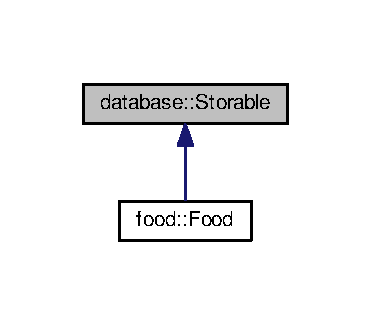
\includegraphics[width=178pt]{classdatabase_1_1_storable__inherit__graph}
\end{center}
\end{figure}
\subsection*{Public Member Functions}
\begin{DoxyCompactItemize}
\item 
virtual auto \hyperlink{classdatabase_1_1_storable_aafaf8ff3b7a854488ae6d4ab3e39f2af}{id} () const -\/$>$ int=0
\item 
virtual auto \hyperlink{classdatabase_1_1_storable_a404fc104e41b9f1e52090a817c7d317e}{name} () const -\/$>$ std\+::string const =0
\item 
virtual void \hyperlink{classdatabase_1_1_storable_afa3a3acb030d9e33064c2f6e34f8bbcf}{set\+\_\+name} (std\+::string\+\_\+view \hyperlink{classdatabase_1_1_storable_a404fc104e41b9f1e52090a817c7d317e}{name})=0
\item 
virtual std\+::string \hyperlink{classdatabase_1_1_storable_a3502dee26cdad8b8e3b0bf1ebc619dc4}{str} () const =0
\item 
virtual auto \hyperlink{classdatabase_1_1_storable_afb1b1572e1147943227794f8abc0d0b0}{get\+\_\+data} () const -\/$>$ \hyperlink{structdatabase_1_1_data}{Data} const =0
\begin{DoxyCompactList}\small\item\em All data will be retrieved from a storable object using this function. \end{DoxyCompactList}\item 
virtual void \hyperlink{classdatabase_1_1_storable_ae554f871860368677cdb3ba5a490c533}{set\+\_\+data} (std\+::vector$<$ \hyperlink{structdatabase_1_1_column_properties}{Column\+Properties} $>$ const \&schema, \hyperlink{structdatabase_1_1_row}{Row} const \&row)=0
\begin{DoxyCompactList}\small\item\em When creating new food objects from data retrieved from the database, this function will be used to set the data for the \hyperlink{classdatabase_1_1_storable}{Storable} object. \end{DoxyCompactList}\item 
virtual \hyperlink{classdatabase_1_1_storable_a9733fea1c4c7070c915444bd924b0975}{$\sim$\+Storable} ()=default
\end{DoxyCompactItemize}


\subsection{Constructor \& Destructor Documentation}
\index{database\+::\+Storable@{database\+::\+Storable}!````~Storable@{$\sim$\+Storable}}
\index{````~Storable@{$\sim$\+Storable}!database\+::\+Storable@{database\+::\+Storable}}
\subsubsection[{\texorpdfstring{$\sim$\+Storable()=default}{~Storable()=default}}]{\setlength{\rightskip}{0pt plus 5cm}virtual database\+::\+Storable\+::$\sim$\+Storable (
\begin{DoxyParamCaption}
{}
\end{DoxyParamCaption}
)\hspace{0.3cm}{\ttfamily [virtual]}, {\ttfamily [default]}}\hypertarget{classdatabase_1_1_storable_a9733fea1c4c7070c915444bd924b0975}{}\label{classdatabase_1_1_storable_a9733fea1c4c7070c915444bd924b0975}


\subsection{Member Function Documentation}
\index{database\+::\+Storable@{database\+::\+Storable}!get\+\_\+data@{get\+\_\+data}}
\index{get\+\_\+data@{get\+\_\+data}!database\+::\+Storable@{database\+::\+Storable}}
\subsubsection[{\texorpdfstring{get\+\_\+data() const -\/$>$ Data const =0}{get_data() const -> Data const =0}}]{\setlength{\rightskip}{0pt plus 5cm}virtual auto database\+::\+Storable\+::get\+\_\+data (
\begin{DoxyParamCaption}
{}
\end{DoxyParamCaption}
) const -\/$>$  {\bf Data} const \hspace{0.3cm}{\ttfamily [pure virtual]}}\hypertarget{classdatabase_1_1_storable_afb1b1572e1147943227794f8abc0d0b0}{}\label{classdatabase_1_1_storable_afb1b1572e1147943227794f8abc0d0b0}


All data will be retrieved from a storable object using this function. 

\begin{DoxyReturn}{Returns}
This A pair containing the column where the data will be store and the data itself. 
\end{DoxyReturn}


Implemented in \hyperlink{classfood_1_1_food_ac3aefc08b78fa521b4317348463e5a5f}{food\+::\+Food}.

\index{database\+::\+Storable@{database\+::\+Storable}!id@{id}}
\index{id@{id}!database\+::\+Storable@{database\+::\+Storable}}
\subsubsection[{\texorpdfstring{id() const -\/$>$ int=0}{id() const -> int=0}}]{\setlength{\rightskip}{0pt plus 5cm}virtual auto database\+::\+Storable\+::id (
\begin{DoxyParamCaption}
{}
\end{DoxyParamCaption}
) const -\/$>$  int\hspace{0.3cm}{\ttfamily [pure virtual]}}\hypertarget{classdatabase_1_1_storable_aafaf8ff3b7a854488ae6d4ab3e39f2af}{}\label{classdatabase_1_1_storable_aafaf8ff3b7a854488ae6d4ab3e39f2af}
\begin{DoxyReturn}{Returns}
The unique ID of the \hyperlink{classdatabase_1_1_storable}{Storable} object 
\end{DoxyReturn}


Implemented in \hyperlink{classfood_1_1_food_a76d21be86ff4500225e593205fc305c5}{food\+::\+Food}.

\index{database\+::\+Storable@{database\+::\+Storable}!name@{name}}
\index{name@{name}!database\+::\+Storable@{database\+::\+Storable}}
\subsubsection[{\texorpdfstring{name() const -\/$>$ std\+::string const =0}{name() const -> std::string const =0}}]{\setlength{\rightskip}{0pt plus 5cm}virtual auto database\+::\+Storable\+::name (
\begin{DoxyParamCaption}
{}
\end{DoxyParamCaption}
) const -\/$>$  std\+::string const \hspace{0.3cm}{\ttfamily [pure virtual]}}\hypertarget{classdatabase_1_1_storable_a404fc104e41b9f1e52090a817c7d317e}{}\label{classdatabase_1_1_storable_a404fc104e41b9f1e52090a817c7d317e}
\begin{DoxyReturn}{Returns}
The name of the food 
\end{DoxyReturn}


Implemented in \hyperlink{classfood_1_1_food_a29ccb0bdf6b74e6073b87bc71c70df04}{food\+::\+Food}.

\index{database\+::\+Storable@{database\+::\+Storable}!set\+\_\+data@{set\+\_\+data}}
\index{set\+\_\+data@{set\+\_\+data}!database\+::\+Storable@{database\+::\+Storable}}
\subsubsection[{\texorpdfstring{set\+\_\+data(std\+::vector$<$ Column\+Properties $>$ const \&schema, Row const \&row)=0}{set_data(std::vector< ColumnProperties > const &schema, Row const &row)=0}}]{\setlength{\rightskip}{0pt plus 5cm}virtual void database\+::\+Storable\+::set\+\_\+data (
\begin{DoxyParamCaption}
\item[{std\+::vector$<$ {\bf Column\+Properties} $>$ const \&}]{schema, }
\item[{{\bf Row} const \&}]{row}
\end{DoxyParamCaption}
)\hspace{0.3cm}{\ttfamily [pure virtual]}}\hypertarget{classdatabase_1_1_storable_ae554f871860368677cdb3ba5a490c533}{}\label{classdatabase_1_1_storable_ae554f871860368677cdb3ba5a490c533}


When creating new food objects from data retrieved from the database, this function will be used to set the data for the \hyperlink{classdatabase_1_1_storable}{Storable} object. 


\begin{DoxyParams}{Parameters}
{\em schema} & A vector containing the properties of each column that make up a schema\\
\hline
{\em data} & A row of data to set the object data \\
\hline
\end{DoxyParams}
\index{database\+::\+Storable@{database\+::\+Storable}!set\+\_\+name@{set\+\_\+name}}
\index{set\+\_\+name@{set\+\_\+name}!database\+::\+Storable@{database\+::\+Storable}}
\subsubsection[{\texorpdfstring{set\+\_\+name(std\+::string\+\_\+view name)=0}{set_name(std::string_view name)=0}}]{\setlength{\rightskip}{0pt plus 5cm}virtual void database\+::\+Storable\+::set\+\_\+name (
\begin{DoxyParamCaption}
\item[{std\+::string\+\_\+view}]{name}
\end{DoxyParamCaption}
)\hspace{0.3cm}{\ttfamily [pure virtual]}}\hypertarget{classdatabase_1_1_storable_afa3a3acb030d9e33064c2f6e34f8bbcf}{}\label{classdatabase_1_1_storable_afa3a3acb030d9e33064c2f6e34f8bbcf}

\begin{DoxyParams}{Parameters}
{\em A} & new name for the food \\
\hline
\end{DoxyParams}


Implemented in \hyperlink{classfood_1_1_food_ac717bda45254fd555b4de00004423041}{food\+::\+Food}.

\index{database\+::\+Storable@{database\+::\+Storable}!str@{str}}
\index{str@{str}!database\+::\+Storable@{database\+::\+Storable}}
\subsubsection[{\texorpdfstring{str() const =0}{str() const =0}}]{\setlength{\rightskip}{0pt plus 5cm}virtual std\+::string database\+::\+Storable\+::str (
\begin{DoxyParamCaption}
{}
\end{DoxyParamCaption}
) const\hspace{0.3cm}{\ttfamily [pure virtual]}}\hypertarget{classdatabase_1_1_storable_a3502dee26cdad8b8e3b0bf1ebc619dc4}{}\label{classdatabase_1_1_storable_a3502dee26cdad8b8e3b0bf1ebc619dc4}
\begin{DoxyReturn}{Returns}
string representation of the name and data, the same way sqlite displays table data 
\end{DoxyReturn}


Implemented in \hyperlink{classfood_1_1_food_a2ac3b444a1ef09dbcec63370f2c8f554}{food\+::\+Food}.



The documentation for this class was generated from the following file\+:\begin{DoxyCompactItemize}
\item 
/home/travis/build/\+Manuel\+Meraz/\+Tracker/include/database/\hyperlink{_storable_8hpp}{Storable.\+hpp}\end{DoxyCompactItemize}

\chapter{File Documentation}
\hypertarget{_data_8hpp}{}\section{/home/travis/build/\+Manuel\+Meraz/\+Tracker/include/database/\+Data.hpp File Reference}
\label{_data_8hpp}\index{/home/travis/build/\+Manuel\+Meraz/\+Tracker/include/database/\+Data.\+hpp@{/home/travis/build/\+Manuel\+Meraz/\+Tracker/include/database/\+Data.\+hpp}}


The container for all data to be stored into a database.  


{\ttfamily \#include $<$ctime$>$}\\*
{\ttfamily \#include $<$string$>$}\\*
{\ttfamily \#include $<$variant$>$}\\*
{\ttfamily \#include $<$vector$>$}\\*
Include dependency graph for Data.\+hpp\+:
\nopagebreak
\begin{figure}[H]
\begin{center}
\leavevmode
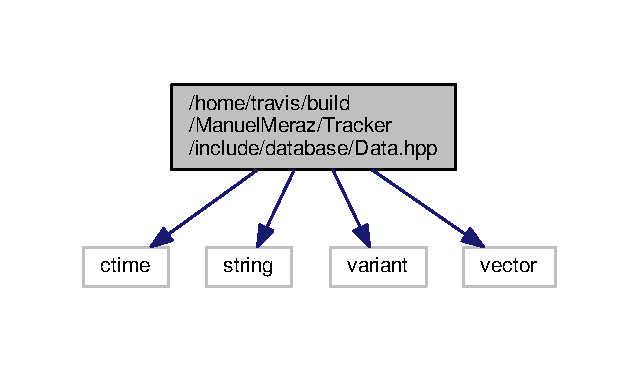
\includegraphics[width=307pt]{_data_8hpp__incl}
\end{center}
\end{figure}
This graph shows which files directly or indirectly include this file\+:
\nopagebreak
\begin{figure}[H]
\begin{center}
\leavevmode
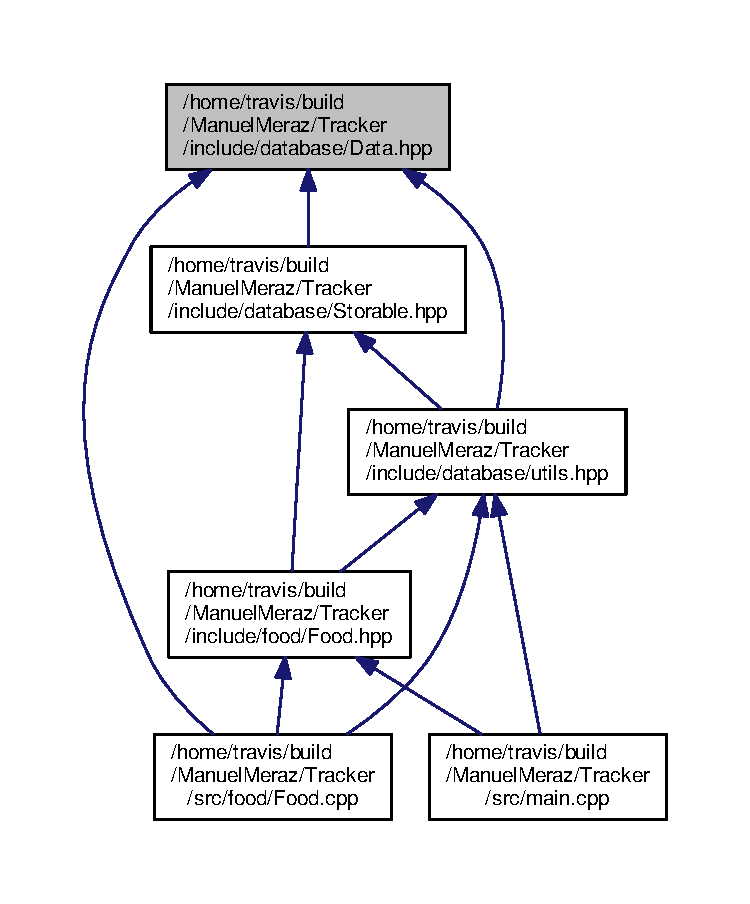
\includegraphics[width=350pt]{_data_8hpp__dep__incl}
\end{center}
\end{figure}
\subsection*{Classes}
\begin{DoxyCompactItemize}
\item 
struct \hyperlink{structdatabase_1_1_column_properties}{database\+::\+Column\+Properties}
\begin{DoxyCompactList}\small\item\em The column properties for a column in a table. A group of these represents a schema. \end{DoxyCompactList}\item 
struct \hyperlink{structdatabase_1_1_row}{database\+::\+Row}
\begin{DoxyCompactList}\small\item\em A row of variant data. \end{DoxyCompactList}\item 
struct \hyperlink{structdatabase_1_1_data}{database\+::\+Data}
\begin{DoxyCompactList}\small\item\em The data to be stored into a database. \end{DoxyCompactList}\end{DoxyCompactItemize}
\subsection*{Namespaces}
\begin{DoxyCompactItemize}
\item 
 \hyperlink{namespacedatabase}{database}
\begin{DoxyCompactList}\small\item\em Organizes all databasing related classes and functions. \end{DoxyCompactList}\end{DoxyCompactItemize}
\subsection*{Enumerations}
\begin{DoxyCompactItemize}
\item 
enum \hyperlink{namespacedatabase_a596cea80c57ec5a9b3b4018f733a43fd}{database\+::\+Data\+Type} \{ \\*
\hyperlink{namespacedatabase_a596cea80c57ec5a9b3b4018f733a43fda8cf125b0e31559ba75a9d9b4f818a554}{database\+::\+Data\+Type\+::\+R\+E\+AL}, 
\hyperlink{namespacedatabase_a596cea80c57ec5a9b3b4018f733a43fda5d5cd46919fa987731fb2edefe0f2a0c}{database\+::\+Data\+Type\+::\+I\+N\+T\+E\+G\+ER}, 
\hyperlink{namespacedatabase_a596cea80c57ec5a9b3b4018f733a43fda61a96ffcb251bb9bf0abf8fec19d0ea8}{database\+::\+Data\+Type\+::\+T\+E\+XT}, 
\hyperlink{namespacedatabase_a596cea80c57ec5a9b3b4018f733a43fda6d67bdfe4ae19f38aff8f363bca42892}{database\+::\+Data\+Type\+::\+N\+U\+L\+L\+\_\+}, 
\\*
\hyperlink{namespacedatabase_a596cea80c57ec5a9b3b4018f733a43fda1649cff06611a6025da3dd511a97fb43}{database\+::\+Data\+Type\+::\+B\+L\+OB}
 \}\begin{DoxyCompactList}\small\item\em S\+QL datatypes that could be stored into a database. \end{DoxyCompactList}
\item 
enum \hyperlink{namespacedatabase_a77defe1118948f64f1e32f4b78c04f5b}{database\+::\+Constraint} \{ \hyperlink{namespacedatabase_a77defe1118948f64f1e32f4b78c04f5ba5e0276ef8ae59ebb9aae19348ad173d5}{database\+::\+Constraint\+::\+P\+R\+I\+M\+A\+R\+Y\+\_\+\+K\+EY}, 
\hyperlink{namespacedatabase_a77defe1118948f64f1e32f4b78c04f5ba88e3e8040c7cd11b9faffdf34372fa2a}{database\+::\+Constraint\+::\+U\+N\+I\+Q\+UE}, 
\hyperlink{namespacedatabase_a77defe1118948f64f1e32f4b78c04f5baeed1de8e53bda49dda97e42841cfe6c5}{database\+::\+Constraint\+::\+N\+O\+T\+\_\+\+N\+U\+LL}, 
\hyperlink{namespacedatabase_a77defe1118948f64f1e32f4b78c04f5ba8c46d8d9d3402788403e2f6911153089}{database\+::\+Constraint\+::\+C\+H\+E\+CK}
 \}\begin{DoxyCompactList}\small\item\em The S\+QL constraint for column of data when creating a table schema. \end{DoxyCompactList}
\end{DoxyCompactItemize}


\subsection{Detailed Description}
The container for all data to be stored into a database. 

\begin{DoxyAuthor}{Author}
Manuel G. Meraz 
\end{DoxyAuthor}
\begin{DoxyDate}{Date}
03/29/2019 
\end{DoxyDate}

\hypertarget{_database_8hpp}{}\section{/home/travis/build/\+Manuel\+Meraz/\+Tracker/include/database/\+Database.hpp File Reference}
\label{_database_8hpp}\index{/home/travis/build/\+Manuel\+Meraz/\+Tracker/include/database/\+Database.\+hpp@{/home/travis/build/\+Manuel\+Meraz/\+Tracker/include/database/\+Database.\+hpp}}


Due to the way S\+Q\+Lite works, we want a single connection to the database up and running at all times. This class keeps the connection maintained.  


{\ttfamily \#include $<$soci-\/sqlite3.\+h$>$}\\*
{\ttfamily \#include $<$soci.\+h$>$}\\*
{\ttfamily \#include $<$memory$>$}\\*
Include dependency graph for Database.\+hpp\+:
\nopagebreak
\begin{figure}[H]
\begin{center}
\leavevmode
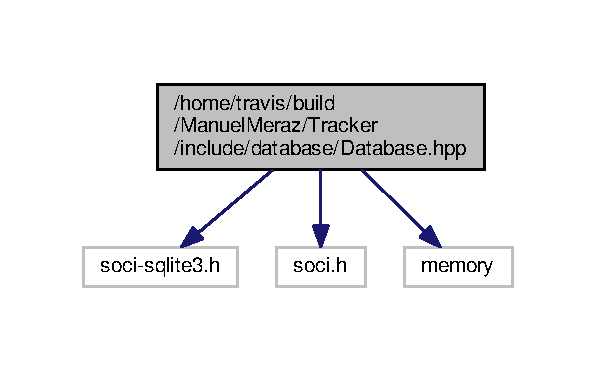
\includegraphics[width=286pt]{_database_8hpp__incl}
\end{center}
\end{figure}
This graph shows which files directly or indirectly include this file\+:
\nopagebreak
\begin{figure}[H]
\begin{center}
\leavevmode
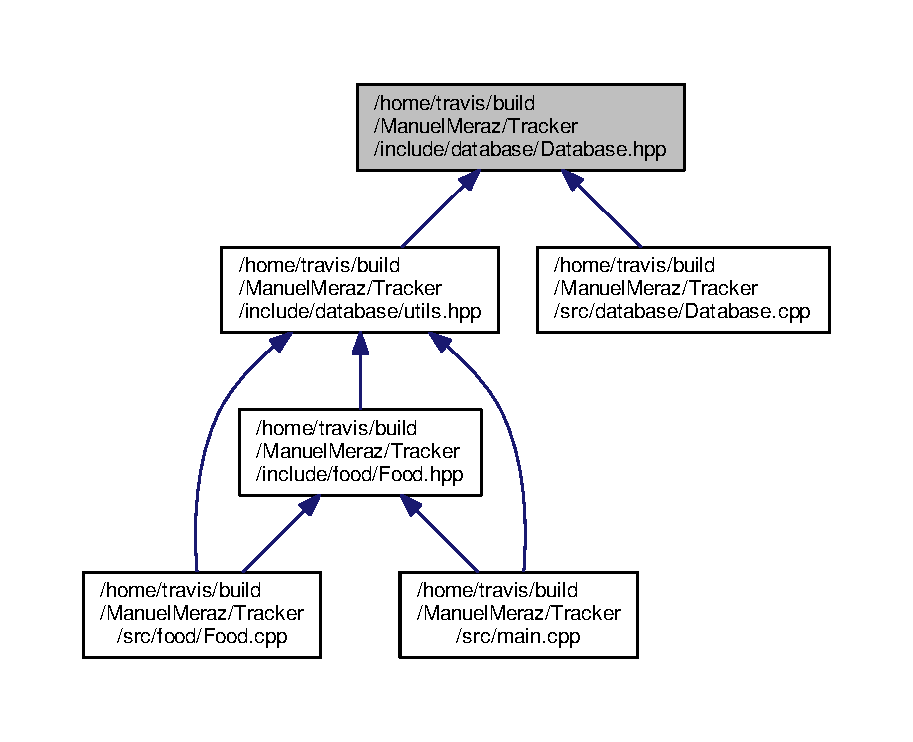
\includegraphics[width=350pt]{_database_8hpp__dep__incl}
\end{center}
\end{figure}
\subsection*{Classes}
\begin{DoxyCompactItemize}
\item 
class \hyperlink{classdatabase_1_1_database}{database\+::\+Database}
\begin{DoxyCompactList}\small\item\em The database singleton class is in charge all database queries. \end{DoxyCompactList}\end{DoxyCompactItemize}
\subsection*{Namespaces}
\begin{DoxyCompactItemize}
\item 
 \hyperlink{namespacedatabase}{database}
\begin{DoxyCompactList}\small\item\em Organizes all databasing related classes and functions. \end{DoxyCompactList}\end{DoxyCompactItemize}


\subsection{Detailed Description}
Due to the way S\+Q\+Lite works, we want a single connection to the database up and running at all times. This class keeps the connection maintained. 

\begin{DoxyAuthor}{Author}
Manuel G. Meraz 
\end{DoxyAuthor}
\begin{DoxyDate}{Date}
03/13/2019 
\end{DoxyDate}

\hypertarget{_storable_8hpp}{}\section{/home/travis/build/\+Manuel\+Meraz/\+Tracker/include/database/\+Storable.hpp File Reference}
\label{_storable_8hpp}\index{/home/travis/build/\+Manuel\+Meraz/\+Tracker/include/database/\+Storable.\+hpp@{/home/travis/build/\+Manuel\+Meraz/\+Tracker/include/database/\+Storable.\+hpp}}


The base class that all storable data will inherit from.  


{\ttfamily \#include \char`\"{}database/\+Data.\+hpp\char`\"{}}\\*
{\ttfamily \#include $<$string$>$}\\*
Include dependency graph for Storable.\+hpp\+:
\nopagebreak
\begin{figure}[H]
\begin{center}
\leavevmode
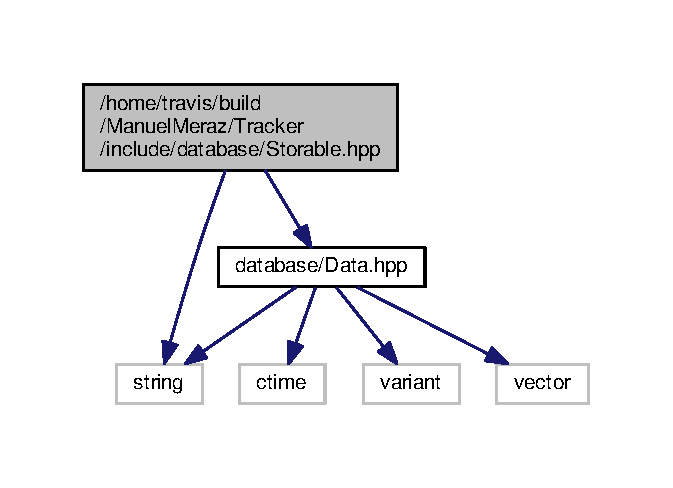
\includegraphics[width=323pt]{_storable_8hpp__incl}
\end{center}
\end{figure}
This graph shows which files directly or indirectly include this file\+:
\nopagebreak
\begin{figure}[H]
\begin{center}
\leavevmode
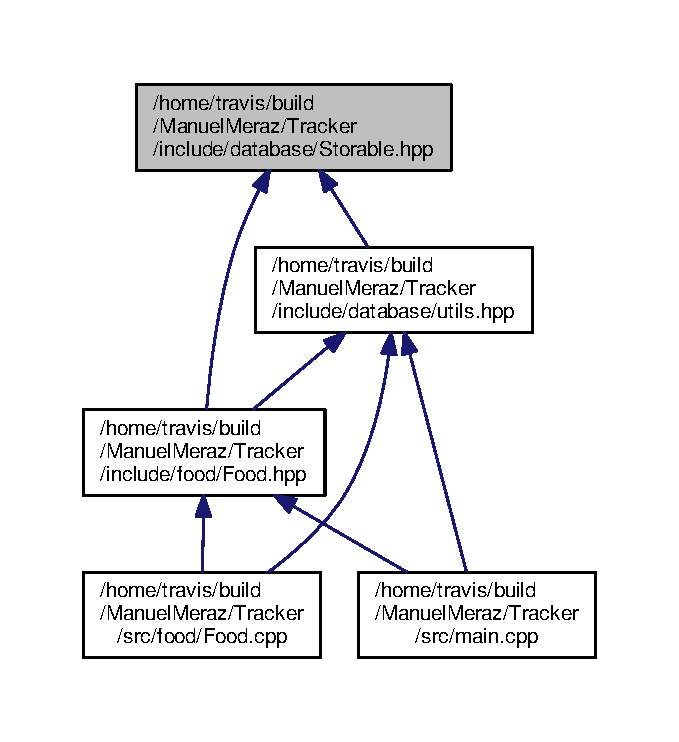
\includegraphics[width=326pt]{_storable_8hpp__dep__incl}
\end{center}
\end{figure}
\subsection*{Classes}
\begin{DoxyCompactItemize}
\item 
class \hyperlink{classdatabase_1_1_storable}{database\+::\+Storable}
\end{DoxyCompactItemize}
\subsection*{Namespaces}
\begin{DoxyCompactItemize}
\item 
 \hyperlink{namespacedatabase}{database}
\begin{DoxyCompactList}\small\item\em Organizes all databasing related classes and functions. \end{DoxyCompactList}\end{DoxyCompactItemize}


\subsection{Detailed Description}
The base class that all storable data will inherit from. 

\begin{DoxyAuthor}{Author}
Manuel G. Meraz 
\end{DoxyAuthor}
\begin{DoxyDate}{Date}
03/11/2019 
\end{DoxyDate}

\hypertarget{utils_8hpp}{}\section{/home/travis/build/\+Manuel\+Meraz/\+Tracker/include/database/utils.hpp File Reference}
\label{utils_8hpp}\index{/home/travis/build/\+Manuel\+Meraz/\+Tracker/include/database/utils.\+hpp@{/home/travis/build/\+Manuel\+Meraz/\+Tracker/include/database/utils.\+hpp}}


Utility functions and objects for databasing.  


{\ttfamily \#include \char`\"{}database/\+Data.\+hpp\char`\"{}}\\*
{\ttfamily \#include \char`\"{}database/\+Database.\+hpp\char`\"{}}\\*
{\ttfamily \#include \char`\"{}database/\+Storable.\+hpp\char`\"{}}\\*
{\ttfamily \#include $<$nameof.\+hpp$>$}\\*
{\ttfamily \#include $<$range/v3/all.\+hpp$>$}\\*
{\ttfamily \#include $<$iostream$>$}\\*
{\ttfamily \#include $<$sstream$>$}\\*
{\ttfamily \#include $<$string\+\_\+view$>$}\\*
{\ttfamily \#include $<$type\+\_\+traits$>$}\\*
{\ttfamily \#include $<$unordered\+\_\+map$>$}\\*
{\ttfamily \#include $<$vector$>$}\\*
Include dependency graph for utils.\+hpp\+:
\nopagebreak
\begin{figure}[H]
\begin{center}
\leavevmode
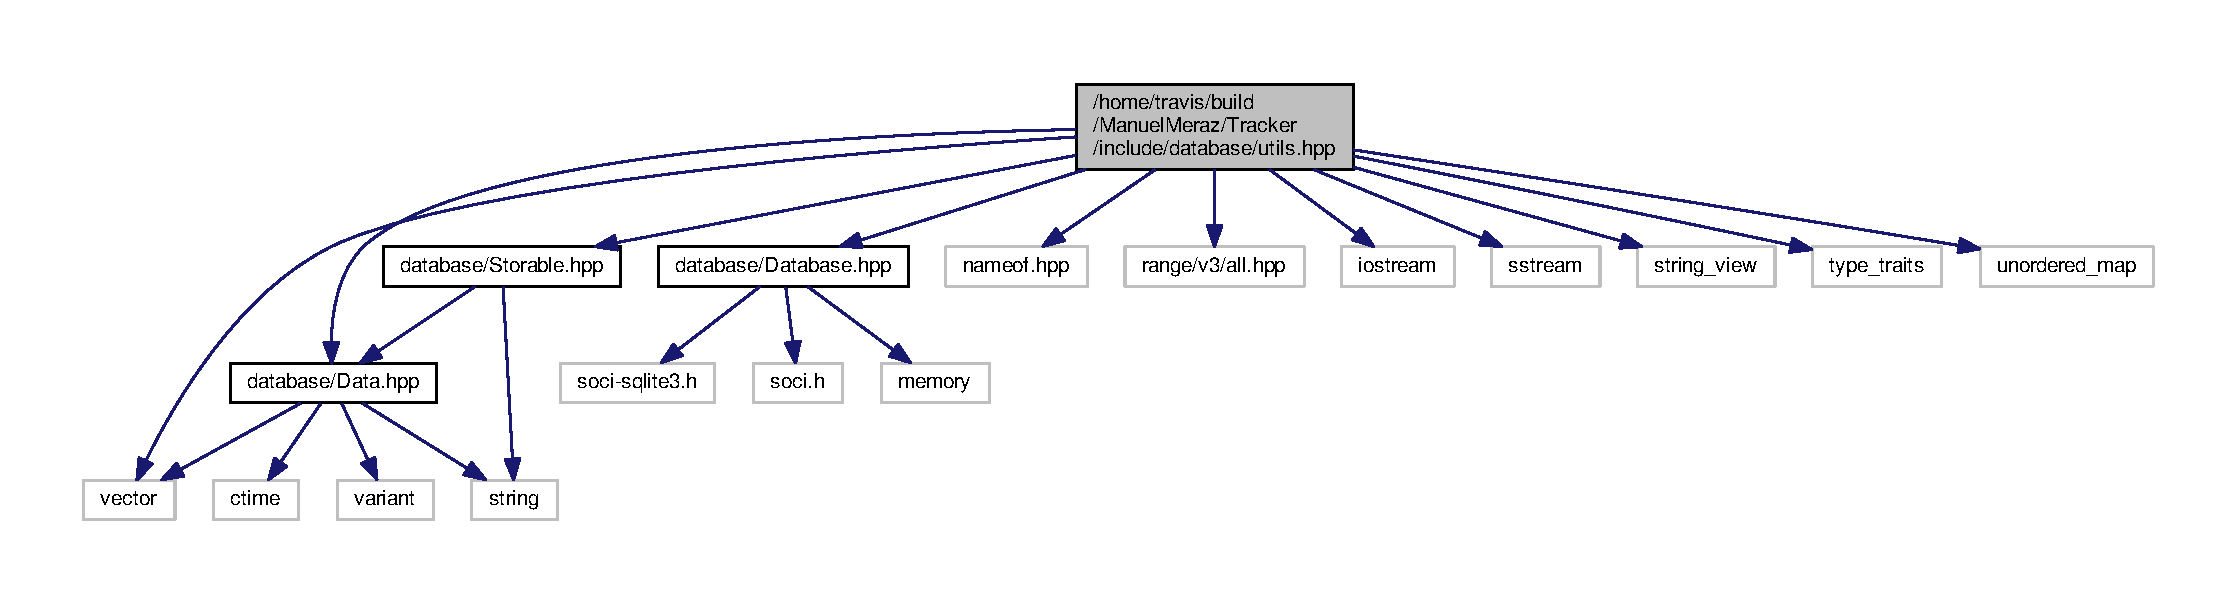
\includegraphics[width=350pt]{utils_8hpp__incl}
\end{center}
\end{figure}
This graph shows which files directly or indirectly include this file\+:
\nopagebreak
\begin{figure}[H]
\begin{center}
\leavevmode
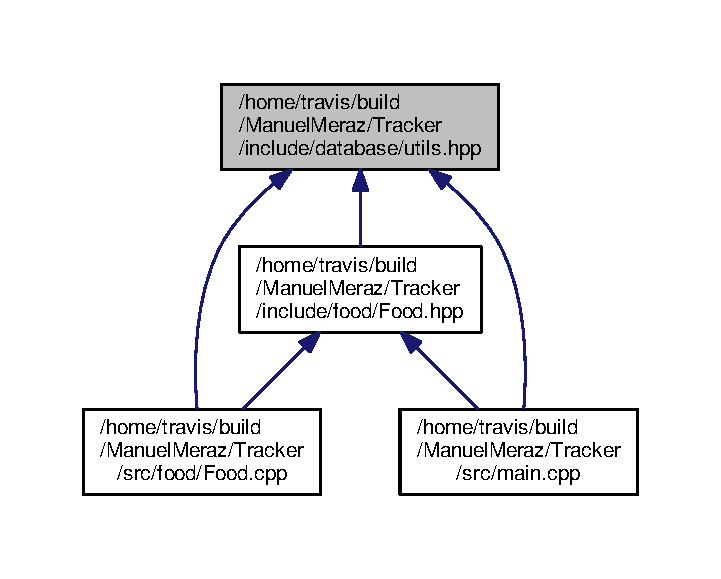
\includegraphics[width=346pt]{utils_8hpp__dep__incl}
\end{center}
\end{figure}
\subsection*{Namespaces}
\begin{DoxyCompactItemize}
\item 
 \hyperlink{namespacedatabase}{database}
\begin{DoxyCompactList}\small\item\em Organizes all databasing related classes and functions. \end{DoxyCompactList}\item 
 \hyperlink{namespacedatabase_1_1utils}{database\+::utils}
\begin{DoxyCompactList}\small\item\em Utility functions to insert, retrieve, and manipulate objects in database. \end{DoxyCompactList}\end{DoxyCompactItemize}
\subsection*{Functions}
\begin{DoxyCompactItemize}
\item 
{\footnotesize template$<$class Forward\+It , class T , class Compare  = std\+::less$<$$>$$>$ }\\auto \hyperlink{namespacedatabase_1_1utils_a0dd569af49c9913a5090b71c86690fe5}{database\+::utils\+::binary\+\_\+find} (Forward\+It first, Forward\+It last, const T \&value, Compare comp) -\/$>$ Forward\+It
\begin{DoxyCompactList}\small\item\em Finds and returns the object if it exists in the stl container. \end{DoxyCompactList}\item 
{\footnotesize template$<$typename Storable , typename std\+::enable\+\_\+if\+\_\+t$<$ std\+::is\+\_\+base\+\_\+of\+\_\+v$<$ database\+::\+Storable, std\+::decay\+\_\+t$<$ Storable $>$$>$, int $>$  = 0$>$ }\\auto \hyperlink{namespacedatabase_1_1utils_adae24cb18f62390528243ff3218d8626}{database\+::utils\+::count\+\_\+rows} () -\/$>$ size\+\_\+t
\begin{DoxyCompactList}\small\item\em Count the number of \hyperlink{classdatabase_1_1_storable}{Storable} type in the database. \end{DoxyCompactList}\item 
{\footnotesize template$<$typename Storable , typename std\+::enable\+\_\+if\+\_\+t$<$ std\+::is\+\_\+base\+\_\+of\+\_\+v$<$ database\+::\+Storable, std\+::decay\+\_\+t$<$ Storable $>$$>$, int $>$  = 0$>$ }\\void \hyperlink{namespacedatabase_1_1utils_a303b59245b11befd59f3fd0e838ef80b}{database\+::utils\+::create\+\_\+table} (std\+::vector$<$ Column\+Properties $>$ const \&schema)
\begin{DoxyCompactList}\small\item\em Create table of \hyperlink{classdatabase_1_1_storable}{Storable} if not exists. \end{DoxyCompactList}\item 
{\footnotesize template$<$typename Storable , typename std\+::enable\+\_\+if\+\_\+t$<$ std\+::is\+\_\+base\+\_\+of\+\_\+v$<$ database\+::\+Storable, std\+::decay\+\_\+t$<$ Storable $>$$>$, int $>$  = 0$>$ }\\void \hyperlink{namespacedatabase_1_1utils_ac56bf4b6fc7b1481c84e42e6bb6db57b}{database\+::utils\+::delete\+\_\+storable} (Storable const \&storable)
\begin{DoxyCompactList}\small\item\em Delete \hyperlink{classdatabase_1_1_storable}{Storable} object from datbase and cache of storables. \end{DoxyCompactList}\item 
{\footnotesize template$<$typename Storable , typename std\+::enable\+\_\+if\+\_\+t$<$ std\+::is\+\_\+base\+\_\+of\+\_\+v$<$ database\+::\+Storable, std\+::decay\+\_\+t$<$ Storable $>$$>$, int $>$  = 0$>$ }\\void \hyperlink{namespacedatabase_1_1utils_abfc70aa38436efb787b6c9f62941856d}{database\+::utils\+::drop\+\_\+table} ()
\begin{DoxyCompactList}\small\item\em Deletes the \hyperlink{classdatabase_1_1_storable}{Storable} table from the database. \end{DoxyCompactList}\item 
{\footnotesize template$<$typename Data\+Enum , typename std\+::enable\+\_\+if\+\_\+t$<$ std\+::is\+\_\+enum\+\_\+v$<$ Data\+Enum $>$, int $>$  = 0$>$ }\\auto \hyperlink{namespacedatabase_1_1utils_a84e6b2503f6453631d2238ff3f9bc9e3}{database\+::utils\+::enum\+\_\+to\+\_\+string} (Data\+Enum const \&data\+\_\+enum) -\/$>$ std\+::string\+\_\+view
\begin{DoxyCompactList}\small\item\em to\+\_\+string function for data enum types \end{DoxyCompactList}\item 
{\footnotesize template$<$typename Storable , typename std\+::enable\+\_\+if\+\_\+t$<$ std\+::is\+\_\+base\+\_\+of\+\_\+v$<$ database\+::\+Storable, std\+::decay\+\_\+t$<$ Storable $>$$>$, int $>$  = 0$>$ }\\auto \hyperlink{namespacedatabase_1_1utils_acab03452308a27ee3e8e5f30842d8ca8}{database\+::utils\+::get\+\_\+new\+\_\+id} () -\/$>$ int
\begin{DoxyCompactList}\small\item\em Generates new unique ID for the type being asked for. \end{DoxyCompactList}\item 
{\footnotesize template$<$typename Storable , typename std\+::enable\+\_\+if\+\_\+t$<$ std\+::is\+\_\+base\+\_\+of\+\_\+v$<$ database\+::\+Storable, std\+::decay\+\_\+t$<$ Storable $>$$>$, int $>$  = 0$>$ }\\void \hyperlink{namespacedatabase_1_1utils_ab9b80f05cca7a094baf577ec5b62108c}{database\+::utils\+::insert} (Storable const \&storable)
\begin{DoxyCompactList}\small\item\em Gets data from any storable object and inserts it into relevant database. \end{DoxyCompactList}\item 
{\footnotesize template$<$typename Storable , typename... Args, typename std\+::enable\+\_\+if\+\_\+t$<$ std\+::is\+\_\+base\+\_\+of\+\_\+v$<$ database\+::\+Storable, std\+::decay\+\_\+t$<$ Storable $>$$>$, int $>$  = 0$>$ }\\auto \hyperlink{namespacedatabase_1_1utils_a8d10f5dbf82b7d8008d8d82865c5a19a}{database\+::utils\+::make} (Args \&\&...args) -\/$>$ Storable \&
\begin{DoxyCompactList}\small\item\em Generates a new \hyperlink{classdatabase_1_1_storable}{Storable} object stores it in the cache, inserts it into the database, and returns a reference to tht new object. \end{DoxyCompactList}\item 
{\footnotesize template$<$typename Storable , typename std\+::enable\+\_\+if\+\_\+t$<$ std\+::is\+\_\+base\+\_\+of\+\_\+v$<$ database\+::\+Storable, std\+::decay\+\_\+t$<$ Storable $>$$>$, int $>$  = 0$>$ }\\auto \hyperlink{namespacedatabase_1_1utils_a41142b70272ad4b4ec442a28dc5c8ce3}{database\+::utils\+::retrieve\+\_\+all} () -\/$>$ std\+::vector$<$ Storable, struct Storable\+::\+Allocator $>$ \&
\begin{DoxyCompactList}\small\item\em Retrieves all database objects that match the \hyperlink{classdatabase_1_1_storable}{Storable} that is passed in. \end{DoxyCompactList}\item 
{\footnotesize template$<$typename Storable , typename std\+::enable\+\_\+if\+\_\+t$<$ std\+::is\+\_\+base\+\_\+of\+\_\+v$<$ database\+::\+Storable, std\+::decay\+\_\+t$<$ Storable $>$$>$, int $>$  = 0$>$ }\\auto \hyperlink{namespacedatabase_1_1utils_a3c5ce09d7fc593c4395d40fe5c1a0630}{database\+::utils\+::table\+\_\+exists} () -\/$>$ bool
\begin{DoxyCompactList}\small\item\em Check if \hyperlink{classdatabase_1_1_storable}{Storable} table exists in database. \end{DoxyCompactList}\item 
{\footnotesize template$<$typename T $>$ }\\auto \hyperlink{namespacedatabase_1_1utils_acb264e8826f50ae828a9c89c2906b049}{database\+::utils\+::type\+\_\+to\+\_\+string} () -\/$>$ std\+::string
\begin{DoxyCompactList}\small\item\em Converts a type to a string and trims the namespaces off. (e.\+g. namespace\+::other\+\_\+namespace\+::\+Class\+Name -\/$>$ \char`\"{}\+Class\+Name\char`\"{}) \end{DoxyCompactList}\item 
{\footnotesize template$<$typename Storable , typename std\+::enable\+\_\+if\+\_\+t$<$ std\+::is\+\_\+base\+\_\+of\+\_\+v$<$ database\+::\+Storable, std\+::decay\+\_\+t$<$ Storable $>$$>$, int $>$  = 0$>$ }\\void \hyperlink{namespacedatabase_1_1utils_ad7fc4b4d352c7b947fc48ac8c1d666a6}{database\+::utils\+::update} (Storable const \&storable)
\begin{DoxyCompactList}\small\item\em Updates the \hyperlink{classdatabase_1_1_storable}{Storable} objects data within the database. \end{DoxyCompactList}\item 
{\footnotesize template$<$typename Lambda $>$ }\\void \hyperlink{namespacedatabase_1_1utils_a974d01a6dbb387b033f627d846630b92}{database\+::utils\+::visit\+\_\+row\+\_\+data} (Lambda const \&handler, Row\+::row\+\_\+data\+\_\+t const \&row\+\_\+data)
\begin{DoxyCompactList}\small\item\em Updates the \hyperlink{classdatabase_1_1_storable}{Storable} objects data within the database. \end{DoxyCompactList}\end{DoxyCompactItemize}


\subsection{Detailed Description}
Utility functions and objects for databasing. 

\begin{DoxyAuthor}{Author}
Manuel G. Meraz 
\end{DoxyAuthor}
\begin{DoxyDate}{Date}
03/30/2019 
\end{DoxyDate}

\hypertarget{_food_8hpp}{}\section{/home/travis/build/\+Manuel\+Meraz/\+Tracker/include/food/\+Food.hpp File Reference}
\label{_food_8hpp}\index{/home/travis/build/\+Manuel\+Meraz/\+Tracker/include/food/\+Food.\+hpp@{/home/travis/build/\+Manuel\+Meraz/\+Tracker/include/food/\+Food.\+hpp}}


The food class stores all macronutrient and micronutrient data for any food.  


{\ttfamily \#include \char`\"{}database/\+Storable.\+hpp\char`\"{}}\\*
{\ttfamily \#include \char`\"{}food/\+Macronutrients.\+hpp\char`\"{}}\\*
{\ttfamily \#include $<$database/utils.\+hpp$>$}\\*
{\ttfamily \#include $<$soci.\+h$>$}\\*
{\ttfamily \#include $<$string$>$}\\*
{\ttfamily \#include $<$string\+\_\+view$>$}\\*
Include dependency graph for Food.\+hpp\+:
\nopagebreak
\begin{figure}[H]
\begin{center}
\leavevmode
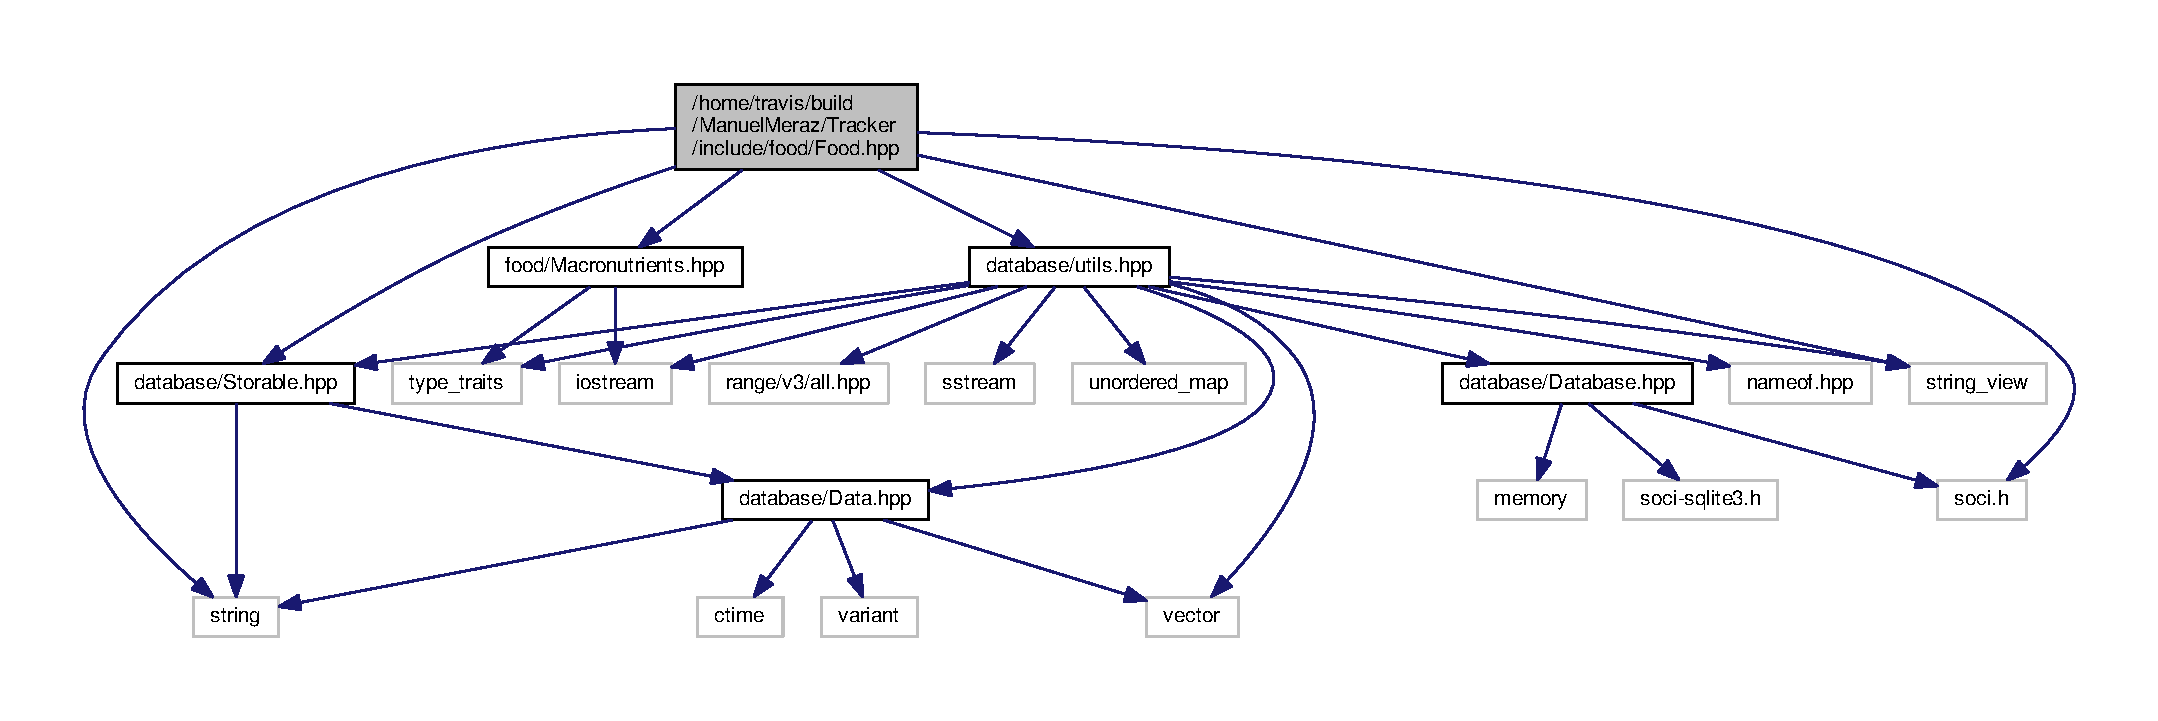
\includegraphics[width=350pt]{_food_8hpp__incl}
\end{center}
\end{figure}
This graph shows which files directly or indirectly include this file\+:
\nopagebreak
\begin{figure}[H]
\begin{center}
\leavevmode
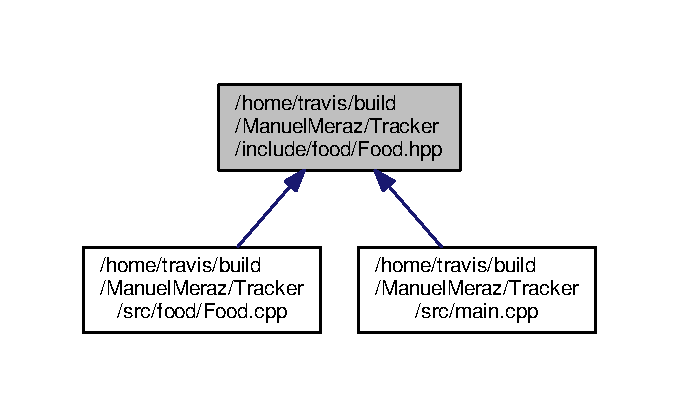
\includegraphics[width=326pt]{_food_8hpp__dep__incl}
\end{center}
\end{figure}
\subsection*{Classes}
\begin{DoxyCompactItemize}
\item 
class \hyperlink{classfood_1_1_food}{food\+::\+Food}
\begin{DoxyCompactList}\small\item\em The food class stores all macronutrient and micronutrient data for any food. \end{DoxyCompactList}\item 
struct \hyperlink{structfood_1_1_food_1_1_allocator}{food\+::\+Food\+::\+Allocator}
\begin{DoxyCompactList}\small\item\em Custom allocator that allows database utils to own a vector of storable objects with private constructors. \end{DoxyCompactList}\item 
struct \hyperlink{structfood_1_1_food_1_1_allocator_1_1rebind}{food\+::\+Food\+::\+Allocator\+::rebind$<$ Food $>$}
\end{DoxyCompactItemize}
\subsection*{Namespaces}
\begin{DoxyCompactItemize}
\item 
 \hyperlink{namespacefood}{food}
\begin{DoxyCompactList}\small\item\em Organizes all food related classes and utilities. \end{DoxyCompactList}\end{DoxyCompactItemize}


\subsection{Detailed Description}
The food class stores all macronutrient and micronutrient data for any food. 

\begin{DoxyAuthor}{Author}
Manuel G. Meraz 
\end{DoxyAuthor}
\begin{DoxyDate}{Date}
03/11/2019 
\end{DoxyDate}

\hypertarget{_macronutrients_8hpp}{}\section{/home/travis/build/\+Manuel\+Meraz/\+Tracker/include/food/\+Macronutrients.hpp File Reference}
\label{_macronutrients_8hpp}\index{/home/travis/build/\+Manuel\+Meraz/\+Tracker/include/food/\+Macronutrients.\+hpp@{/home/travis/build/\+Manuel\+Meraz/\+Tracker/include/food/\+Macronutrients.\+hpp}}
{\ttfamily \#include $<$iostream$>$}\\*
{\ttfamily \#include $<$type\+\_\+traits$>$}\\*
Include dependency graph for Macronutrients.\+hpp\+:
\nopagebreak
\begin{figure}[H]
\begin{center}
\leavevmode
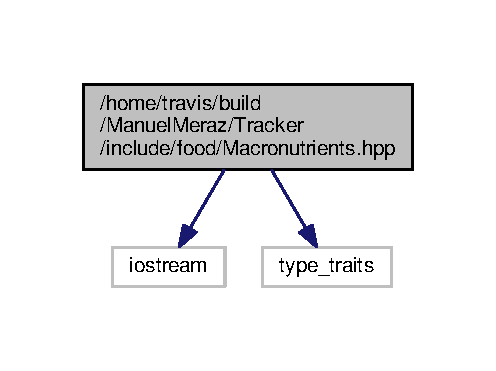
\includegraphics[width=238pt]{_macronutrients_8hpp__incl}
\end{center}
\end{figure}
This graph shows which files directly or indirectly include this file\+:
\nopagebreak
\begin{figure}[H]
\begin{center}
\leavevmode
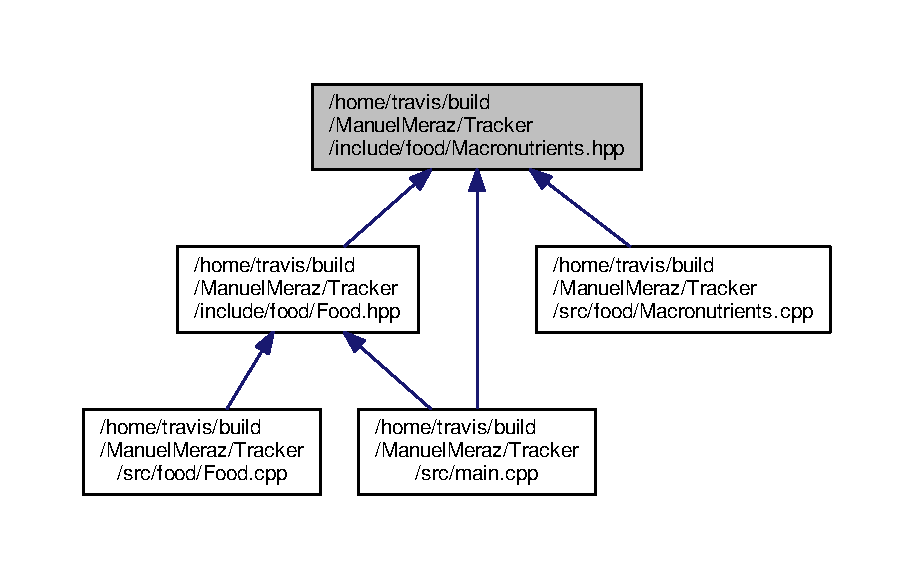
\includegraphics[width=350pt]{_macronutrients_8hpp__dep__incl}
\end{center}
\end{figure}
\subsection*{Classes}
\begin{DoxyCompactItemize}
\item 
struct \hyperlink{structfood_1_1_fat}{food\+::\+Fat}
\begin{DoxyCompactList}\small\item\em Stores the fat content of a food. \end{DoxyCompactList}\item 
struct \hyperlink{structfood_1_1_fiber}{food\+::\+Fiber}
\begin{DoxyCompactList}\small\item\em Stores the fiber content of a food. \end{DoxyCompactList}\item 
struct \hyperlink{structfood_1_1_carbohydrate}{food\+::\+Carbohydrate}
\begin{DoxyCompactList}\small\item\em Stores the carbohydrate content of a food. \end{DoxyCompactList}\item 
struct \hyperlink{structfood_1_1_protein}{food\+::\+Protein}
\begin{DoxyCompactList}\small\item\em Stores the protein content of a food. \end{DoxyCompactList}\item 
class \hyperlink{classfood_1_1_macronutrients}{food\+::\+Macronutrients}
\begin{DoxyCompactList}\small\item\em The macronutrients class stores all macronutrient data to be stored in a \hyperlink{classfood_1_1_food}{Food} object. \end{DoxyCompactList}\end{DoxyCompactItemize}
\subsection*{Namespaces}
\begin{DoxyCompactItemize}
\item 
 \hyperlink{namespacefood}{food}
\begin{DoxyCompactList}\small\item\em Organizes all food related classes and utilities. \end{DoxyCompactList}\end{DoxyCompactItemize}

\hypertarget{_r_e_a_d_m_e_8md}{}\section{/home/travis/build/\+Manuel\+Meraz/\+Tracker/\+R\+E\+A\+D\+ME.md File Reference}
\label{_r_e_a_d_m_e_8md}\index{/home/travis/build/\+Manuel\+Meraz/\+Tracker/\+R\+E\+A\+D\+M\+E.\+md@{/home/travis/build/\+Manuel\+Meraz/\+Tracker/\+R\+E\+A\+D\+M\+E.\+md}}

\hypertarget{_database_8cpp}{}\section{/home/travis/build/\+Manuel\+Meraz/\+Tracker/src/database/\+Database.cpp File Reference}
\label{_database_8cpp}\index{/home/travis/build/\+Manuel\+Meraz/\+Tracker/src/database/\+Database.\+cpp@{/home/travis/build/\+Manuel\+Meraz/\+Tracker/src/database/\+Database.\+cpp}}


The database singleton class is in charge all database queries.  


{\ttfamily \#include \char`\"{}database/\+Database.\+hpp\char`\"{}}\\*
{\ttfamily \#include $<$iostream$>$}\\*
Include dependency graph for Database.\+cpp\+:
\nopagebreak
\begin{figure}[H]
\begin{center}
\leavevmode
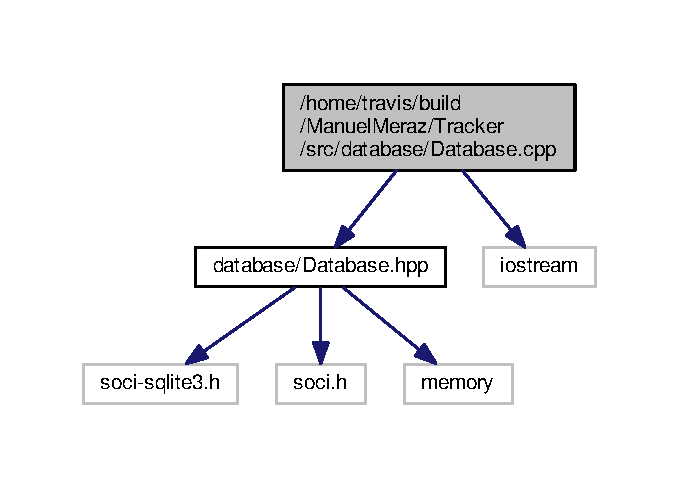
\includegraphics[width=326pt]{_database_8cpp__incl}
\end{center}
\end{figure}


\subsection{Detailed Description}
The database singleton class is in charge all database queries. 

\begin{DoxyAuthor}{Author}
Manuel G. Meraz 
\end{DoxyAuthor}
\begin{DoxyDate}{Date}
03/30/2019 Due to the way S\+Q\+Lite works, we want a single connection to the database up and running at all times. This class keeps the connection maintained. 
\end{DoxyDate}

\hypertarget{_food_8cpp}{}\section{/home/travis/build/\+Manuel\+Meraz/\+Tracker/src/food/\+Food.cpp File Reference}
\label{_food_8cpp}\index{/home/travis/build/\+Manuel\+Meraz/\+Tracker/src/food/\+Food.\+cpp@{/home/travis/build/\+Manuel\+Meraz/\+Tracker/src/food/\+Food.\+cpp}}


The food class stores all macronutrient and micronutrient data for any food.  


{\ttfamily \#include \char`\"{}food/\+Food.\+hpp\char`\"{}}\\*
{\ttfamily \#include \char`\"{}database/\+Data.\+hpp\char`\"{}}\\*
{\ttfamily \#include \char`\"{}database/utils.\+hpp\char`\"{}}\\*
{\ttfamily \#include $<$range/v3/all.\+hpp$>$}\\*
{\ttfamily \#include $<$sstream$>$}\\*
{\ttfamily \#include $<$unordered\+\_\+map$>$}\\*
Include dependency graph for Food.\+cpp\+:
\nopagebreak
\begin{figure}[H]
\begin{center}
\leavevmode
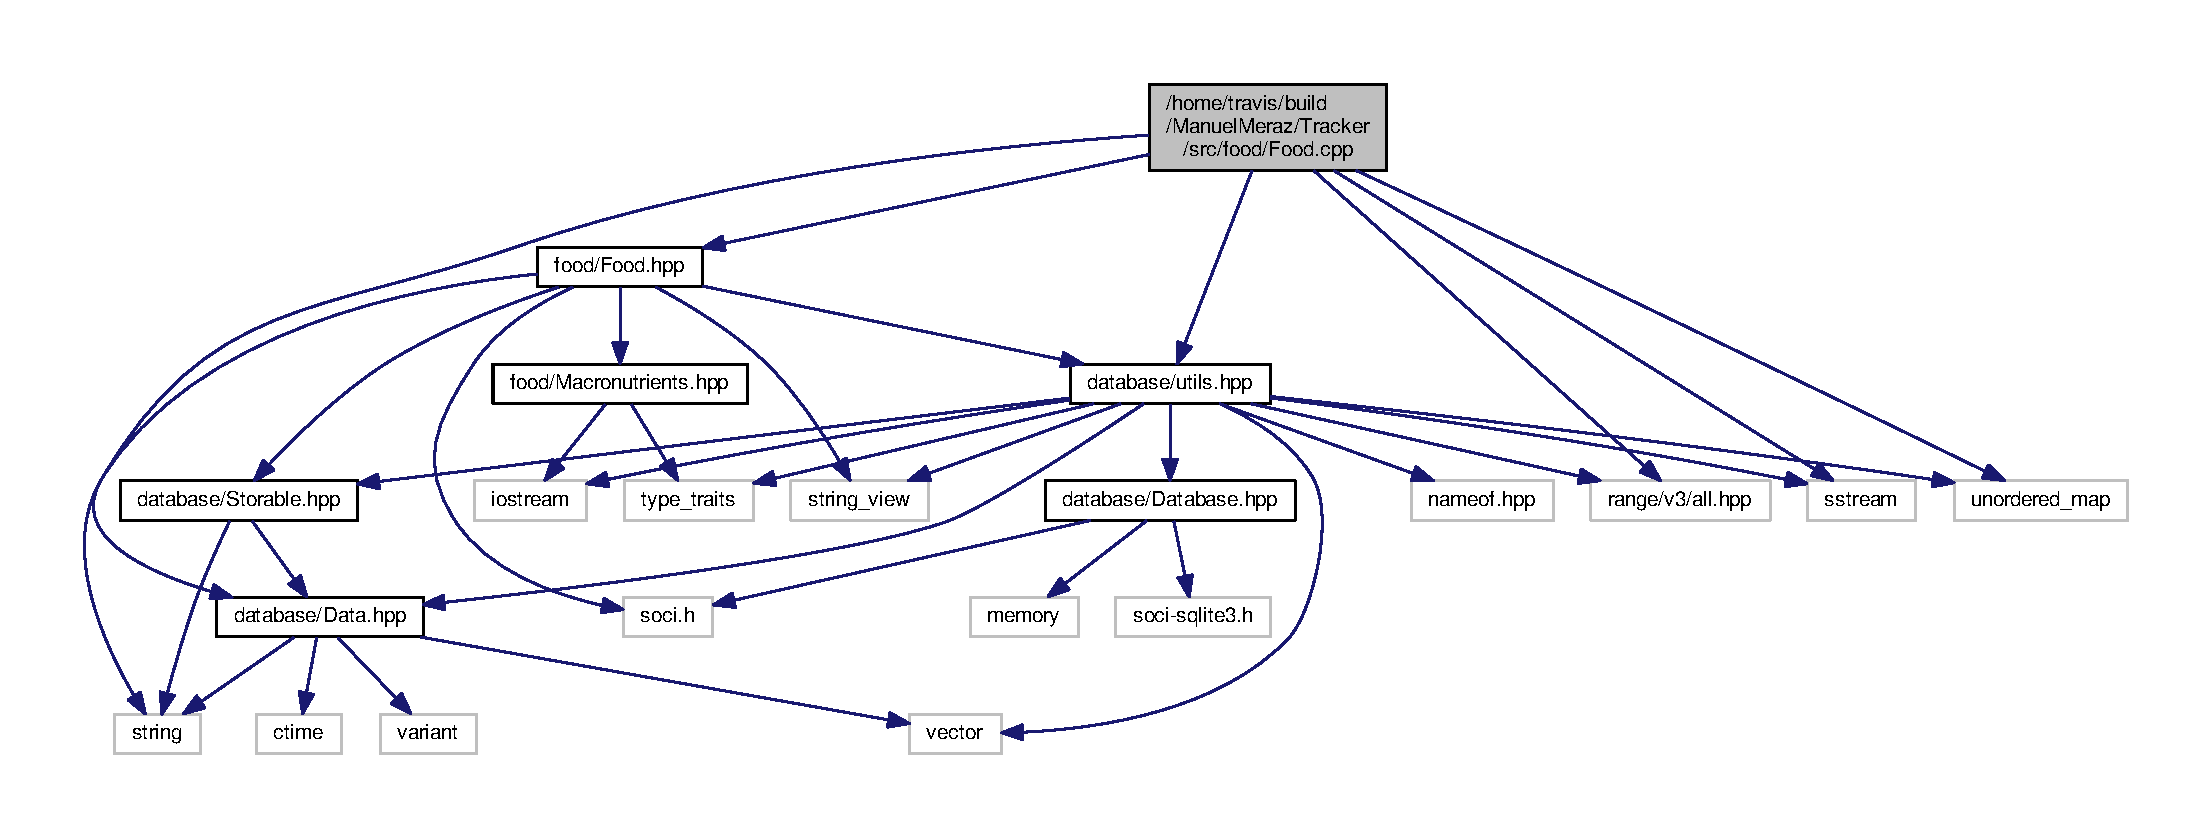
\includegraphics[width=350pt]{_food_8cpp__incl}
\end{center}
\end{figure}


\subsection{Detailed Description}
The food class stores all macronutrient and micronutrient data for any food. 

\begin{DoxyAuthor}{Author}
Manuel G. Meraz 
\end{DoxyAuthor}
\begin{DoxyDate}{Date}
03/29/2019 
\end{DoxyDate}

\hypertarget{_macronutrients_8cpp}{}\section{/home/travis/build/\+Manuel\+Meraz/\+Tracker/src/food/\+Macronutrients.cpp File Reference}
\label{_macronutrients_8cpp}\index{/home/travis/build/\+Manuel\+Meraz/\+Tracker/src/food/\+Macronutrients.\+cpp@{/home/travis/build/\+Manuel\+Meraz/\+Tracker/src/food/\+Macronutrients.\+cpp}}


Contains the Macronutrients class and related helper classes food.  


{\ttfamily \#include \char`\"{}food/\+Macronutrients.\+hpp\char`\"{}}\\*
Include dependency graph for Macronutrients.\+cpp\+:
\nopagebreak
\begin{figure}[H]
\begin{center}
\leavevmode
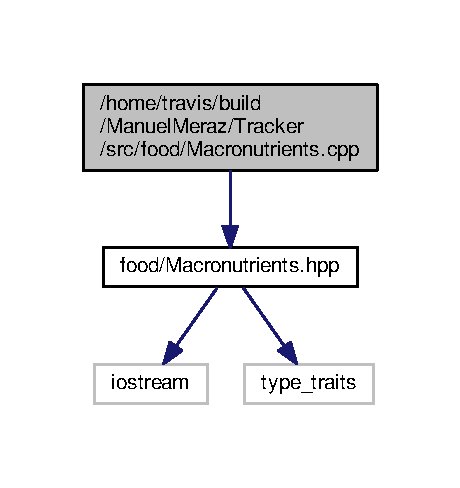
\includegraphics[width=221pt]{_macronutrients_8cpp__incl}
\end{center}
\end{figure}


\subsection{Detailed Description}
Contains the Macronutrients class and related helper classes food. 

\begin{DoxyAuthor}{Author}
Manuel G. Meraz 
\end{DoxyAuthor}
\begin{DoxyDate}{Date}
04/10/2019 
\end{DoxyDate}

\hypertarget{main_8cpp}{}\section{/home/travis/build/\+Manuel\+Meraz/\+Tracker/src/main.cpp File Reference}
\label{main_8cpp}\index{/home/travis/build/\+Manuel\+Meraz/\+Tracker/src/main.\+cpp@{/home/travis/build/\+Manuel\+Meraz/\+Tracker/src/main.\+cpp}}
{\ttfamily \#include \char`\"{}database/utils.\+hpp\char`\"{}}\\*
{\ttfamily \#include \char`\"{}food/\+Food.\+hpp\char`\"{}}\\*
{\ttfamily \#include \char`\"{}food/\+Macronutrients.\+hpp\char`\"{}}\\*
Include dependency graph for main.\+cpp\+:
\nopagebreak
\begin{figure}[H]
\begin{center}
\leavevmode
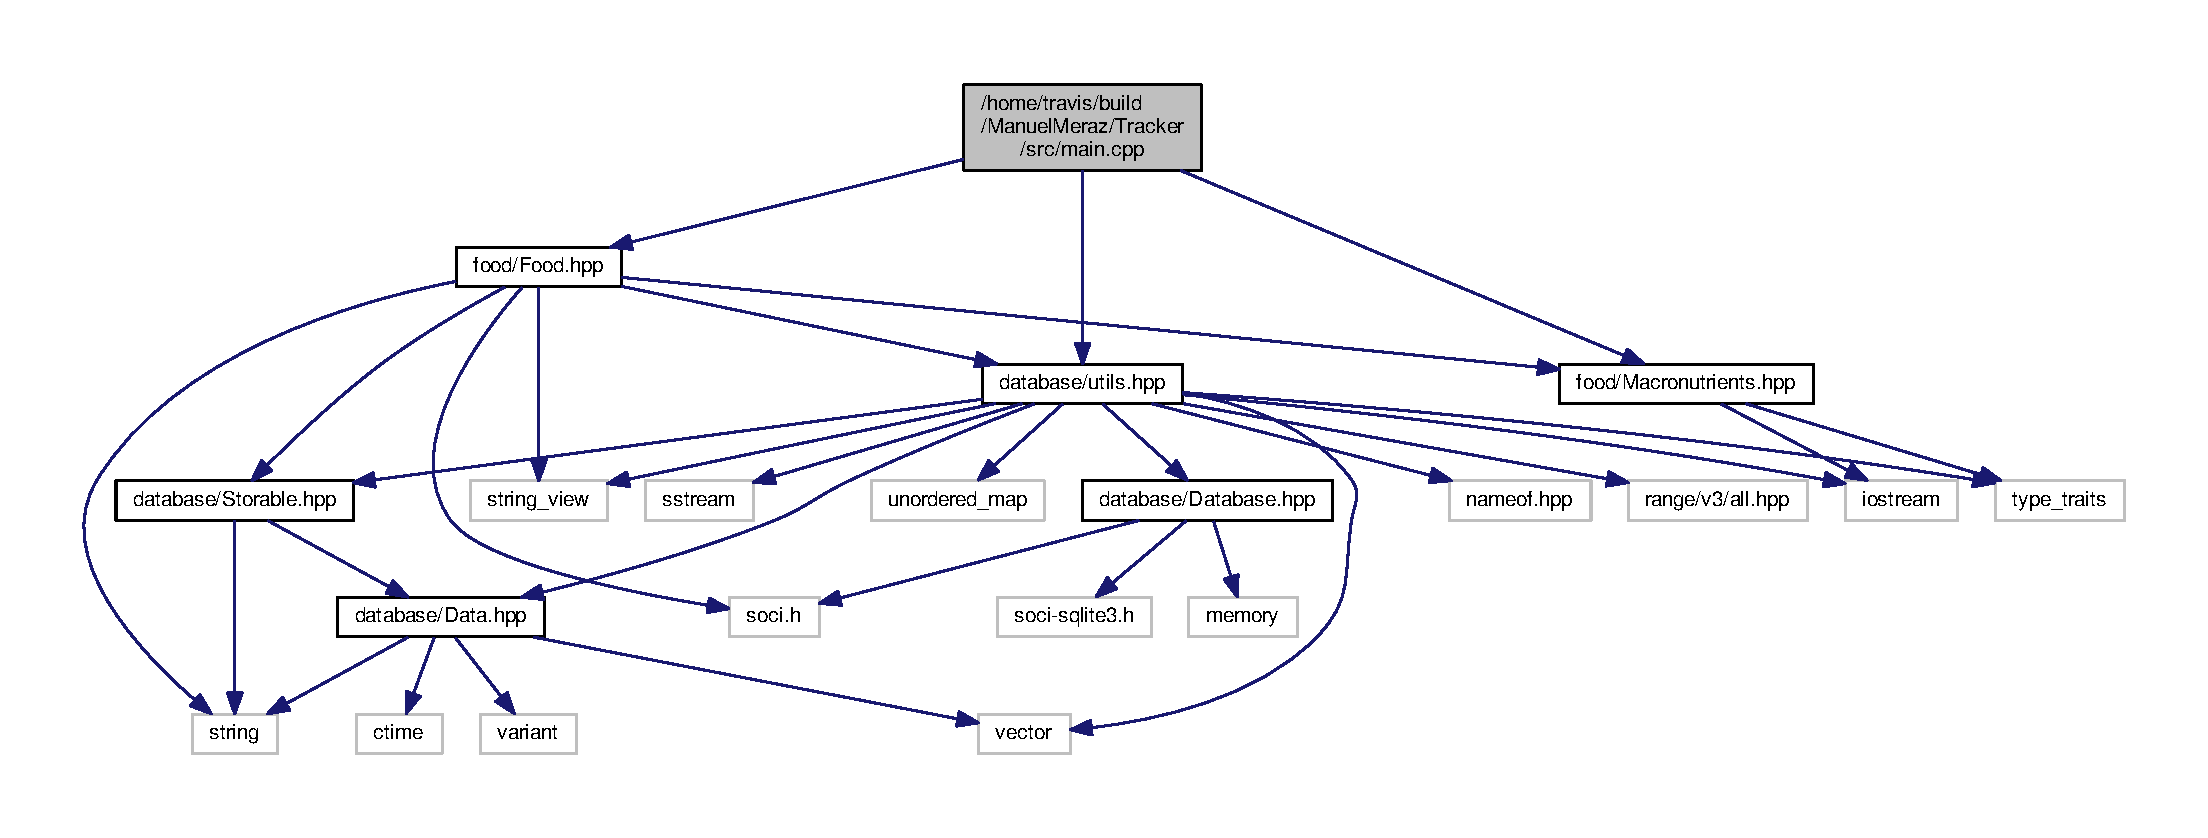
\includegraphics[width=350pt]{main_8cpp__incl}
\end{center}
\end{figure}
\subsection*{Functions}
\begin{DoxyCompactItemize}
\item 
auto \hyperlink{main_8cpp_a8216c1645620cdb2f629cde3ac02ffef}{main} () -\/$>$ int
\end{DoxyCompactItemize}


\subsection{Function Documentation}
\index{main.\+cpp@{main.\+cpp}!main@{main}}
\index{main@{main}!main.\+cpp@{main.\+cpp}}
\subsubsection[{\texorpdfstring{main() -\/$>$ int}{main() -> int}}]{\setlength{\rightskip}{0pt plus 5cm}auto main (
\begin{DoxyParamCaption}
{}
\end{DoxyParamCaption}
) -\/$>$ int
}\hypertarget{main_8cpp_a8216c1645620cdb2f629cde3ac02ffef}{}\label{main_8cpp_a8216c1645620cdb2f629cde3ac02ffef}

\hypertarget{test-food_8cpp}{}\section{/home/travis/build/\+Manuel\+Meraz/\+Tracker/tests/test-\/food.cpp File Reference}
\label{test-food_8cpp}\index{/home/travis/build/\+Manuel\+Meraz/\+Tracker/tests/test-\/food.\+cpp@{/home/travis/build/\+Manuel\+Meraz/\+Tracker/tests/test-\/food.\+cpp}}
{\ttfamily \#include \char`\"{}gtest/gtest.\+h\char`\"{}}\\*
Include dependency graph for test-\/food.cpp\+:
\nopagebreak
\begin{figure}[H]
\begin{center}
\leavevmode
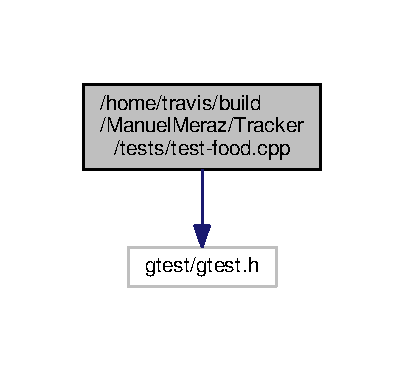
\includegraphics[width=194pt]{test-food_8cpp__incl}
\end{center}
\end{figure}
\subsection*{Functions}
\begin{DoxyCompactItemize}
\item 
\hyperlink{test-food_8cpp_a954e68bbfbfc207bc80d6ae782a35f28}{T\+E\+ST} (Test\+Suite, Test)
\item 
auto \hyperlink{test-food_8cpp_a808f40e2e9d6eb5463165c031dfa3eb1}{main} (int argc, char $\ast$$\ast$argv) -\/$>$ int
\end{DoxyCompactItemize}


\subsection{Function Documentation}
\index{test-\/food.\+cpp@{test-\/food.\+cpp}!main@{main}}
\index{main@{main}!test-\/food.\+cpp@{test-\/food.\+cpp}}
\subsubsection[{\texorpdfstring{main(int argc, char $\ast$$\ast$argv) -\/$>$ int}{main(int argc, char **argv) -> int}}]{\setlength{\rightskip}{0pt plus 5cm}auto main (
\begin{DoxyParamCaption}
\item[{int}]{argc, }
\item[{char $\ast$$\ast$}]{argv}
\end{DoxyParamCaption}
) -\/$>$ int
}\hypertarget{test-food_8cpp_a808f40e2e9d6eb5463165c031dfa3eb1}{}\label{test-food_8cpp_a808f40e2e9d6eb5463165c031dfa3eb1}
\index{test-\/food.\+cpp@{test-\/food.\+cpp}!T\+E\+ST@{T\+E\+ST}}
\index{T\+E\+ST@{T\+E\+ST}!test-\/food.\+cpp@{test-\/food.\+cpp}}
\subsubsection[{\texorpdfstring{T\+E\+S\+T(\+Test\+Suite, Test)}{TEST(TestSuite, Test)}}]{\setlength{\rightskip}{0pt plus 5cm}T\+E\+ST (
\begin{DoxyParamCaption}
\item[{Test\+Suite}]{, }
\item[{Test}]{}
\end{DoxyParamCaption}
)}\hypertarget{test-food_8cpp_a954e68bbfbfc207bc80d6ae782a35f28}{}\label{test-food_8cpp_a954e68bbfbfc207bc80d6ae782a35f28}

%--- End generated contents ---

% Index
\backmatter
\newpage
\phantomsection
\clearemptydoublepage
\addcontentsline{toc}{chapter}{Index}
\printindex

\end{document}
